


% Header, overrides base

    % Make sure that the sphinx doc style knows who it inherits from.
    \def\sphinxdocclass{article}

    % Declare the document class
    \documentclass[letterpaper,10pt,english]{/Users/polarwander/Library/Enthought/Canopy_64bit/User/lib/python2.7/site-packages/sphinx/texinputs/sphinxhowto}

    % Imports
    \usepackage[utf8]{inputenc}
    \DeclareUnicodeCharacter{00A0}{\\nobreakspace}
    \usepackage[T1]{fontenc}
    \usepackage{babel}
    \usepackage{times}
    \usepackage{import}
    \usepackage[Bjarne]{/Users/polarwander/Library/Enthought/Canopy_64bit/User/lib/python2.7/site-packages/sphinx/texinputs/fncychap}
    \usepackage{longtable}
    \usepackage{/Users/polarwander/Library/Enthought/Canopy_64bit/User/lib/python2.7/site-packages/sphinx/texinputs/sphinx}
    \usepackage{multirow}

    \usepackage{amsmath}
    \usepackage{amssymb}
    \usepackage{ucs}
    \usepackage{enumerate}

    % Used to make the Input/Output rules follow around the contents.
    \usepackage{needspace}

    % Pygments requirements
    \usepackage{fancyvrb}
    \usepackage{color}
    % ansi colors additions
    \definecolor{darkgreen}{rgb}{.12,.54,.11}
    \definecolor{lightgray}{gray}{.95}
    \definecolor{brown}{rgb}{0.54,0.27,0.07}
    \definecolor{purple}{rgb}{0.5,0.0,0.5}
    \definecolor{darkgray}{gray}{0.25}
    \definecolor{lightred}{rgb}{1.0,0.39,0.28}
    \definecolor{lightgreen}{rgb}{0.48,0.99,0.0}
    \definecolor{lightblue}{rgb}{0.53,0.81,0.92}
    \definecolor{lightpurple}{rgb}{0.87,0.63,0.87}
    \definecolor{lightcyan}{rgb}{0.5,1.0,0.83}

    % Needed to box output/input
    \usepackage{tikz}
        \usetikzlibrary{calc,arrows,shadows}
    \usepackage[framemethod=tikz]{mdframed}

    \usepackage{alltt}

    % Used to load and display graphics
    \usepackage{graphicx}
    \graphicspath{ {figs/} }
    \usepackage[Export]{adjustbox} % To resize

    % used so that images for notebooks which have spaces in the name can still be included
    \usepackage{grffile}


    % For formatting output while also word wrapping.
    \usepackage{listings}
    \lstset{breaklines=true}
    \lstset{basicstyle=\small\ttfamily}
    \def\smaller{\fontsize{9.5pt}{9.5pt}\selectfont}

    %Pygments definitions
    
\makeatletter
\def\PY@reset{\let\PY@it=\relax \let\PY@bf=\relax%
    \let\PY@ul=\relax \let\PY@tc=\relax%
    \let\PY@bc=\relax \let\PY@ff=\relax}
\def\PY@tok#1{\csname PY@tok@#1\endcsname}
\def\PY@toks#1+{\ifx\relax#1\empty\else%
    \PY@tok{#1}\expandafter\PY@toks\fi}
\def\PY@do#1{\PY@bc{\PY@tc{\PY@ul{%
    \PY@it{\PY@bf{\PY@ff{#1}}}}}}}
\def\PY#1#2{\PY@reset\PY@toks#1+\relax+\PY@do{#2}}

\expandafter\def\csname PY@tok@gd\endcsname{\def\PY@tc##1{\textcolor[rgb]{0.63,0.00,0.00}{##1}}}
\expandafter\def\csname PY@tok@gu\endcsname{\let\PY@bf=\textbf\def\PY@tc##1{\textcolor[rgb]{0.50,0.00,0.50}{##1}}}
\expandafter\def\csname PY@tok@gt\endcsname{\def\PY@tc##1{\textcolor[rgb]{0.00,0.27,0.87}{##1}}}
\expandafter\def\csname PY@tok@gs\endcsname{\let\PY@bf=\textbf}
\expandafter\def\csname PY@tok@gr\endcsname{\def\PY@tc##1{\textcolor[rgb]{1.00,0.00,0.00}{##1}}}
\expandafter\def\csname PY@tok@cm\endcsname{\let\PY@it=\textit\def\PY@tc##1{\textcolor[rgb]{0.25,0.50,0.50}{##1}}}
\expandafter\def\csname PY@tok@vg\endcsname{\def\PY@tc##1{\textcolor[rgb]{0.10,0.09,0.49}{##1}}}
\expandafter\def\csname PY@tok@m\endcsname{\def\PY@tc##1{\textcolor[rgb]{0.40,0.40,0.40}{##1}}}
\expandafter\def\csname PY@tok@mh\endcsname{\def\PY@tc##1{\textcolor[rgb]{0.40,0.40,0.40}{##1}}}
\expandafter\def\csname PY@tok@go\endcsname{\def\PY@tc##1{\textcolor[rgb]{0.53,0.53,0.53}{##1}}}
\expandafter\def\csname PY@tok@ge\endcsname{\let\PY@it=\textit}
\expandafter\def\csname PY@tok@vc\endcsname{\def\PY@tc##1{\textcolor[rgb]{0.10,0.09,0.49}{##1}}}
\expandafter\def\csname PY@tok@il\endcsname{\def\PY@tc##1{\textcolor[rgb]{0.40,0.40,0.40}{##1}}}
\expandafter\def\csname PY@tok@cs\endcsname{\let\PY@it=\textit\def\PY@tc##1{\textcolor[rgb]{0.25,0.50,0.50}{##1}}}
\expandafter\def\csname PY@tok@cp\endcsname{\def\PY@tc##1{\textcolor[rgb]{0.74,0.48,0.00}{##1}}}
\expandafter\def\csname PY@tok@gi\endcsname{\def\PY@tc##1{\textcolor[rgb]{0.00,0.63,0.00}{##1}}}
\expandafter\def\csname PY@tok@gh\endcsname{\let\PY@bf=\textbf\def\PY@tc##1{\textcolor[rgb]{0.00,0.00,0.50}{##1}}}
\expandafter\def\csname PY@tok@ni\endcsname{\let\PY@bf=\textbf\def\PY@tc##1{\textcolor[rgb]{0.60,0.60,0.60}{##1}}}
\expandafter\def\csname PY@tok@nl\endcsname{\def\PY@tc##1{\textcolor[rgb]{0.63,0.63,0.00}{##1}}}
\expandafter\def\csname PY@tok@nn\endcsname{\let\PY@bf=\textbf\def\PY@tc##1{\textcolor[rgb]{0.00,0.00,1.00}{##1}}}
\expandafter\def\csname PY@tok@no\endcsname{\def\PY@tc##1{\textcolor[rgb]{0.53,0.00,0.00}{##1}}}
\expandafter\def\csname PY@tok@na\endcsname{\def\PY@tc##1{\textcolor[rgb]{0.49,0.56,0.16}{##1}}}
\expandafter\def\csname PY@tok@nb\endcsname{\def\PY@tc##1{\textcolor[rgb]{0.00,0.50,0.00}{##1}}}
\expandafter\def\csname PY@tok@nc\endcsname{\let\PY@bf=\textbf\def\PY@tc##1{\textcolor[rgb]{0.00,0.00,1.00}{##1}}}
\expandafter\def\csname PY@tok@nd\endcsname{\def\PY@tc##1{\textcolor[rgb]{0.67,0.13,1.00}{##1}}}
\expandafter\def\csname PY@tok@ne\endcsname{\let\PY@bf=\textbf\def\PY@tc##1{\textcolor[rgb]{0.82,0.25,0.23}{##1}}}
\expandafter\def\csname PY@tok@nf\endcsname{\def\PY@tc##1{\textcolor[rgb]{0.00,0.00,1.00}{##1}}}
\expandafter\def\csname PY@tok@si\endcsname{\let\PY@bf=\textbf\def\PY@tc##1{\textcolor[rgb]{0.73,0.40,0.53}{##1}}}
\expandafter\def\csname PY@tok@s2\endcsname{\def\PY@tc##1{\textcolor[rgb]{0.73,0.13,0.13}{##1}}}
\expandafter\def\csname PY@tok@vi\endcsname{\def\PY@tc##1{\textcolor[rgb]{0.10,0.09,0.49}{##1}}}
\expandafter\def\csname PY@tok@nt\endcsname{\let\PY@bf=\textbf\def\PY@tc##1{\textcolor[rgb]{0.00,0.50,0.00}{##1}}}
\expandafter\def\csname PY@tok@nv\endcsname{\def\PY@tc##1{\textcolor[rgb]{0.10,0.09,0.49}{##1}}}
\expandafter\def\csname PY@tok@s1\endcsname{\def\PY@tc##1{\textcolor[rgb]{0.73,0.13,0.13}{##1}}}
\expandafter\def\csname PY@tok@sh\endcsname{\def\PY@tc##1{\textcolor[rgb]{0.73,0.13,0.13}{##1}}}
\expandafter\def\csname PY@tok@sc\endcsname{\def\PY@tc##1{\textcolor[rgb]{0.73,0.13,0.13}{##1}}}
\expandafter\def\csname PY@tok@sx\endcsname{\def\PY@tc##1{\textcolor[rgb]{0.00,0.50,0.00}{##1}}}
\expandafter\def\csname PY@tok@bp\endcsname{\def\PY@tc##1{\textcolor[rgb]{0.00,0.50,0.00}{##1}}}
\expandafter\def\csname PY@tok@c1\endcsname{\let\PY@it=\textit\def\PY@tc##1{\textcolor[rgb]{0.25,0.50,0.50}{##1}}}
\expandafter\def\csname PY@tok@kc\endcsname{\let\PY@bf=\textbf\def\PY@tc##1{\textcolor[rgb]{0.00,0.50,0.00}{##1}}}
\expandafter\def\csname PY@tok@c\endcsname{\let\PY@it=\textit\def\PY@tc##1{\textcolor[rgb]{0.25,0.50,0.50}{##1}}}
\expandafter\def\csname PY@tok@mf\endcsname{\def\PY@tc##1{\textcolor[rgb]{0.40,0.40,0.40}{##1}}}
\expandafter\def\csname PY@tok@err\endcsname{\def\PY@bc##1{\setlength{\fboxsep}{0pt}\fcolorbox[rgb]{1.00,0.00,0.00}{1,1,1}{\strut ##1}}}
\expandafter\def\csname PY@tok@kd\endcsname{\let\PY@bf=\textbf\def\PY@tc##1{\textcolor[rgb]{0.00,0.50,0.00}{##1}}}
\expandafter\def\csname PY@tok@ss\endcsname{\def\PY@tc##1{\textcolor[rgb]{0.10,0.09,0.49}{##1}}}
\expandafter\def\csname PY@tok@sr\endcsname{\def\PY@tc##1{\textcolor[rgb]{0.73,0.40,0.53}{##1}}}
\expandafter\def\csname PY@tok@mo\endcsname{\def\PY@tc##1{\textcolor[rgb]{0.40,0.40,0.40}{##1}}}
\expandafter\def\csname PY@tok@kn\endcsname{\let\PY@bf=\textbf\def\PY@tc##1{\textcolor[rgb]{0.00,0.50,0.00}{##1}}}
\expandafter\def\csname PY@tok@mi\endcsname{\def\PY@tc##1{\textcolor[rgb]{0.40,0.40,0.40}{##1}}}
\expandafter\def\csname PY@tok@gp\endcsname{\let\PY@bf=\textbf\def\PY@tc##1{\textcolor[rgb]{0.00,0.00,0.50}{##1}}}
\expandafter\def\csname PY@tok@o\endcsname{\def\PY@tc##1{\textcolor[rgb]{0.40,0.40,0.40}{##1}}}
\expandafter\def\csname PY@tok@kr\endcsname{\let\PY@bf=\textbf\def\PY@tc##1{\textcolor[rgb]{0.00,0.50,0.00}{##1}}}
\expandafter\def\csname PY@tok@s\endcsname{\def\PY@tc##1{\textcolor[rgb]{0.73,0.13,0.13}{##1}}}
\expandafter\def\csname PY@tok@kp\endcsname{\def\PY@tc##1{\textcolor[rgb]{0.00,0.50,0.00}{##1}}}
\expandafter\def\csname PY@tok@w\endcsname{\def\PY@tc##1{\textcolor[rgb]{0.73,0.73,0.73}{##1}}}
\expandafter\def\csname PY@tok@kt\endcsname{\def\PY@tc##1{\textcolor[rgb]{0.69,0.00,0.25}{##1}}}
\expandafter\def\csname PY@tok@ow\endcsname{\let\PY@bf=\textbf\def\PY@tc##1{\textcolor[rgb]{0.67,0.13,1.00}{##1}}}
\expandafter\def\csname PY@tok@sb\endcsname{\def\PY@tc##1{\textcolor[rgb]{0.73,0.13,0.13}{##1}}}
\expandafter\def\csname PY@tok@k\endcsname{\let\PY@bf=\textbf\def\PY@tc##1{\textcolor[rgb]{0.00,0.50,0.00}{##1}}}
\expandafter\def\csname PY@tok@se\endcsname{\let\PY@bf=\textbf\def\PY@tc##1{\textcolor[rgb]{0.73,0.40,0.13}{##1}}}
\expandafter\def\csname PY@tok@sd\endcsname{\let\PY@it=\textit\def\PY@tc##1{\textcolor[rgb]{0.73,0.13,0.13}{##1}}}

\def\PYZbs{\char`\\}
\def\PYZus{\char`\_}
\def\PYZob{\char`\{}
\def\PYZcb{\char`\}}
\def\PYZca{\char`\^}
\def\PYZam{\char`\&}
\def\PYZlt{\char`\<}
\def\PYZgt{\char`\>}
\def\PYZsh{\char`\#}
\def\PYZpc{\char`\%}
\def\PYZdl{\char`\$}
\def\PYZhy{\char`\-}
\def\PYZsq{\char`\'}
\def\PYZdq{\char`\"}
\def\PYZti{\char`\~}
% for compatibility with earlier versions
\def\PYZat{@}
\def\PYZlb{[}
\def\PYZrb{]}
\makeatother


    %Set pygments styles if needed...
    
        \definecolor{nbframe-border}{rgb}{0.867,0.867,0.867}
        \definecolor{nbframe-bg}{rgb}{0.969,0.969,0.969}
        \definecolor{nbframe-in-prompt}{rgb}{0.0,0.0,0.502}
        \definecolor{nbframe-out-prompt}{rgb}{0.545,0.0,0.0}

        \newenvironment{ColorVerbatim}
        {\begin{mdframed}[%
            roundcorner=1.0pt, %
            backgroundcolor=nbframe-bg, %
            userdefinedwidth=1\linewidth, %
            leftmargin=0.1\linewidth, %
            innerleftmargin=0pt, %
            innerrightmargin=0pt, %
            linecolor=nbframe-border, %
            linewidth=1pt, %
            usetwoside=false, %
            everyline=true, %
            innerlinewidth=3pt, %
            innerlinecolor=nbframe-bg, %
            middlelinewidth=1pt, %
            middlelinecolor=nbframe-bg, %
            outerlinewidth=0.5pt, %
            outerlinecolor=nbframe-border, %
            needspace=0pt
        ]}
        {\end{mdframed}}
        
        \newenvironment{InvisibleVerbatim}
        {\begin{mdframed}[leftmargin=0.1\linewidth,innerleftmargin=3pt,innerrightmargin=3pt, userdefinedwidth=1\linewidth, linewidth=0pt, linecolor=white, usetwoside=false]}
        {\end{mdframed}}

        \renewenvironment{Verbatim}[1][\unskip]
        {\begin{alltt}\smaller}
        {\end{alltt}}
    

    % Help prevent overflowing lines due to urls and other hard-to-break 
    % entities.  This doesn't catch everything...
    \sloppy

    % Document level variables
    \title{2014\_Osler\_Data\_Analysis}
    \renewcommand{\releasename}{}

    % TODO: Add option for the user to specify a logo for his/her export.
    \newcommand{\sphinxlogo}{}

    % Make the index page of the document.
    \makeindex

    % Import sphinx document type specifics.
     


% Body

    % Start of the document
    \begin{document}

        
            \maketitle
        

        


        
        \part{Analysis of Simpson Island paleomagnetic data}Corresponding Author: Nicholas L. Swanson-Hysell
(swanson-hysell@berkeley.edu)\section{Introduction}This IPython notebook contains data analysis on paleomagnetic data
developed from ca. 1.1 billion year old lava flows of the Osler Volcanic
Group that are part of the North American Midcontinent Rift. This
analysis accompanies a manuscript under review at \textbf{Geochemistry,
Geophysics, Geosystems} entitled ``Significant plate motion during the
early magmatic stage of North American Midcontinent Rift development''
by N. L. Swanson-Hysell, A. A. Vaughan, M. R. Mustain and K. Asp. This
notebook is part of the supporting online materials and is available at
\url{https://github.com/Swanson-Hysell/2014_Swanson-Hysell-et-al_Osler}
along with the necessary files to execute all of the code. Within this
github repository are the following folders:

\begin{enumerate}
\def\labelenumi{\arabic{enumi}.}
\itemsep1pt\parskip0pt\parsep0pt
\item
  \href{https://github.com/Swanson-Hysell/2014_Swanson-Hysell-et-al_Osler/tree/master/2014_Osler_Code}{2014\_Osler\_Code}
  This folder contains this notebook file as well as necessary
  libraries.
\item
  \href{https://github.com/Swanson-Hysell/2014_Swanson-Hysell-et-al_Osler/tree/master/2014_Osler_Data}{2014\_Osler\_Data}
  This folder contains the data generated in the study at the specimen
  level as well as the flow means that are imported into this notebook
  for data analysis.
\item
  \href{https://github.com/Swanson-Hysell/2014_Swanson-Hysell-et-al_Osler/tree/master/2014_Osler_Manuscript}{2014\_Osler\_Manuscript}
  This folder contains that manuscript text and figures.
\end{enumerate}

If you are viewing this supporting material as a PDF document and want
to run the code in the notebook you will need to download the code from
the github repository and you will also need a Python distribution that
includes IPython (http://ipython.org). Alternatively you can view the
notebook online with the the IPython nbviewer at this link:
http://bit.ly/19XRdjJ\section{Import libraries}This code blocks imports necessary libraries that define functions that
will be used in the data analysis below. The code below uses the pmag.py
and pmagplotlib.py files of the the PmagPy software package (version
pmagpy-2.206) authored by Lisa Tauxe (https://github.com/ltauxe/PmagPy).
The check\_updates and get\_version functions of the PmagPy libraries
cause errors in the interactive environment of IPython so the code below
calls a slightly modified version that is included in the Github
repository for this work. There are other functions that are necessary
for the interactive plotting of paleomagnetic data (some of them edited
from PmagPy) that are within the IPmag.py library that is imported in
the code block below.

    % Make sure that atleast 4 lines are below the HR
    \needspace{4\baselineskip}

    
        \vspace{6pt}
        \makebox[0.1\linewidth]{\smaller\hfill\tt\color{nbframe-in-prompt}In\hspace{4pt}{[}1{]}:\hspace{4pt}}\\*
        \vspace{-2.65\baselineskip}
        \begin{ColorVerbatim}
            \vspace{-0.7\baselineskip}
            \begin{Verbatim}[commandchars=\\\{\}]
\PY{c}{\PYZsh{}import paleomagnetic specific libraries}
\PY{k+kn}{import} \PY{n+nn}{pmag}\PY{o}{,} \PY{n+nn}{pmagplotlib}\PY{o}{,} \PY{n+nn}{IPmag}
\end{Verbatim}

            
                \vspace{-0.2\baselineskip}
            
        \end{ColorVerbatim}
    
This notebook runs with pylab inline which imports the numpy, scipy and
matplotlib functions and allows for the plots to be viewed inline in the
IPython notebook (instead of opening up in another window).

    % Make sure that atleast 4 lines are below the HR
    \needspace{4\baselineskip}

    
        \vspace{6pt}
        \makebox[0.1\linewidth]{\smaller\hfill\tt\color{nbframe-in-prompt}In\hspace{4pt}{[}2{]}:\hspace{4pt}}\\*
        \vspace{-2.65\baselineskip}
        \begin{ColorVerbatim}
            \vspace{-0.7\baselineskip}
            \begin{Verbatim}[commandchars=\\\{\}]
\PY{o}{\PYZpc{}}\PY{k}{pylab} \PY{n}{inline}
\end{Verbatim}

            
                \vspace{-0.2\baselineskip}
            
        \end{ColorVerbatim}
    

    

        % If the first block is an image, minipage the image.  Else
        % request a certain amount of space for the input text.
        \needspace{4\baselineskip}
        
        

            % Add document contents.
            
                \begin{InvisibleVerbatim}
                \vspace{-0.5\baselineskip}
\begin{alltt}Populating the interactive namespace from numpy and matplotlib
\end{alltt}

            \end{InvisibleVerbatim}
            
        
    
\section{Import Simpson Island paleomagnetic data}The data file FlowDataAll.csv has data in the format:

SITE

STRAT\_HEIGHT

DEC\_GEO

INC\_GEO

Dec\_TC

INC\_TC

A95

n

Plat

ABS\_Plat

VGP\_lat

VGP\_long

These data are displayed in a table below and imported by variable in
the cell below the table.

    % Make sure that atleast 4 lines are below the HR
    \needspace{4\baselineskip}

    
        \vspace{6pt}
        \makebox[0.1\linewidth]{\smaller\hfill\tt\color{nbframe-in-prompt}In\hspace{4pt}{[}3{]}:\hspace{4pt}}\\*
        \vspace{-2.65\baselineskip}
        \begin{ColorVerbatim}
            \vspace{-0.7\baselineskip}
            \begin{Verbatim}[commandchars=\\\{\}]
\PY{k+kn}{import} \PY{n+nn}{pandas}
\PY{k+kn}{from} \PY{n+nn}{IPython.core.display} \PY{k+kn}{import} \PY{n}{HTML}
\PY{n}{pandas}\PY{o}{.}\PY{n}{set\PYZus{}option}\PY{p}{(}\PY{l+s}{\PYZsq{}}\PY{l+s}{max\PYZus{}columns}\PY{l+s}{\PYZsq{}}\PY{p}{,} \PY{l+m+mi}{10}\PY{p}{)}

\PY{n}{data} \PY{o}{=} \PY{n}{pandas}\PY{o}{.}\PY{n}{read\PYZus{}csv}\PY{p}{(}\PY{l+s}{\PYZsq{}}\PY{l+s}{../2014\PYZus{}Osler\PYZus{}Data/SimpsonIsland\PYZus{}OslerData.csv}\PY{l+s}{\PYZsq{}}\PY{p}{)}
\PY{n}{display}\PY{p}{(}\PY{n}{HTML}\PY{p}{(}\PY{n}{data}\PY{o}{.}\PY{n}{to\PYZus{}html}\PY{p}{(}\PY{p}{)}\PY{p}{)}\PY{p}{)}
\end{Verbatim}

            
                \vspace{-0.2\baselineskip}
            
        \end{ColorVerbatim}
    

    

        % If the first block is an image, minipage the image.  Else
        % request a certain amount of space for the input text.
        \needspace{4\baselineskip}
        
        

            % Add document contents.
            
                \begin{InvisibleVerbatim}
                \vspace{-0.5\baselineskip}
\begin{alltt}<IPython.core.display.HTML at 0x100436f90>\end{alltt}

            \end{InvisibleVerbatim}
            
        
    


    % Make sure that atleast 4 lines are below the HR
    \needspace{4\baselineskip}

    
        \vspace{6pt}
        \makebox[0.1\linewidth]{\smaller\hfill\tt\color{nbframe-in-prompt}In\hspace{4pt}{[}4{]}:\hspace{4pt}}\\*
        \vspace{-2.65\baselineskip}
        \begin{ColorVerbatim}
            \vspace{-0.7\baselineskip}
            \begin{Verbatim}[commandchars=\\\{\}]
\PY{n}{data\PYZus{}file}\PY{o}{=}\PY{l+s}{\PYZsq{}}\PY{l+s}{../2014\PYZus{}Osler\PYZus{}Data/SimpsonIsland\PYZus{}OslerData.csv}\PY{l+s}{\PYZsq{}}
\PY{n}{SimpsonIsland\PYZus{}Strat} \PY{o}{=} \PY{n}{np}\PY{o}{.}\PY{n}{genfromtxt}\PY{p}{(}\PY{n}{data\PYZus{}file}\PY{p}{,}\PY{n}{delimiter}\PY{o}{=}\PY{l+s}{\PYZdq{}}\PY{l+s}{,}\PY{l+s}{\PYZdq{}}\PY{p}{,} \PY{n}{skip\PYZus{}header}\PY{o}{=}\PY{l+m+mi}{1}\PY{p}{)}

\PY{n}{strat\PYZus{}height}\PY{o}{=}\PY{n}{SimpsonIsland\PYZus{}Strat}\PY{p}{[}\PY{p}{:}\PY{p}{,}\PY{l+m+mi}{1}\PY{p}{]}
\PY{n}{Dec\PYZus{}TC}\PY{o}{=}\PY{n}{SimpsonIsland\PYZus{}Strat}\PY{p}{[}\PY{p}{:}\PY{p}{,}\PY{l+m+mi}{6}\PY{p}{]}
\PY{n}{Inc\PYZus{}TC}\PY{o}{=}\PY{n}{SimpsonIsland\PYZus{}Strat}\PY{p}{[}\PY{p}{:}\PY{p}{,}\PY{l+m+mi}{7}\PY{p}{]}
\PY{n}{A95}\PY{o}{=}\PY{n}{SimpsonIsland\PYZus{}Strat}\PY{p}{[}\PY{p}{:}\PY{p}{,}\PY{l+m+mi}{8}\PY{p}{]}
\PY{n}{plat}\PY{o}{=}\PY{n}{SimpsonIsland\PYZus{}Strat}\PY{p}{[}\PY{p}{:}\PY{p}{,}\PY{l+m+mi}{10}\PY{p}{]}
\PY{n}{abs\PYZus{}plat}\PY{o}{=}\PY{n}{SimpsonIsland\PYZus{}Strat}\PY{p}{[}\PY{p}{:}\PY{p}{,}\PY{l+m+mi}{11}\PY{p}{]}
\PY{n}{VGP\PYZus{}lat}\PY{o}{=}\PY{n}{SimpsonIsland\PYZus{}Strat}\PY{p}{[}\PY{p}{:}\PY{p}{,}\PY{l+m+mi}{12}\PY{p}{]}
\PY{n}{VGP\PYZus{}long}\PY{o}{=}\PY{n}{SimpsonIsland\PYZus{}Strat}\PY{p}{[}\PY{p}{:}\PY{p}{,}\PY{l+m+mi}{13}\PY{p}{]}
\end{Verbatim}

            
                \vspace{-0.2\baselineskip}
            
        \end{ColorVerbatim}
    
\section{Comparison between data from the lower 1/3, middle 1/3 and upper 1/3 of
Simpson Island stratigraphy}Let's consider the data by stratigraphically grouping flow data from the
lower third (0 to 1041 meters), middle third (1041 to 2083 meters) and
the upper third (2083 to 3124 meters) of the stratigraphy. The Fisher
means for these groups are calculated with the data being displayed on
equal area plots with these means.

    % Make sure that atleast 4 lines are below the HR
    \needspace{4\baselineskip}

    
        \vspace{6pt}
        \makebox[0.1\linewidth]{\smaller\hfill\tt\color{nbframe-in-prompt}In\hspace{4pt}{[}5{]}:\hspace{4pt}}\\*
        \vspace{-2.65\baselineskip}
        \begin{ColorVerbatim}
            \vspace{-0.7\baselineskip}
            \begin{Verbatim}[commandchars=\\\{\}]
\PY{n}{SI\PYZus{}Directions}\PY{o}{=}\PY{p}{[}\PY{p}{]}
\PY{n}{SI\PYZus{}Poles}\PY{o}{=}\PY{p}{[}\PY{p}{]}

\PY{k}{for} \PY{n}{n} \PY{o+ow}{in} \PY{n+nb}{range}\PY{p}{(}\PY{l+m+mi}{0}\PY{p}{,}\PY{l+m+mi}{84}\PY{p}{)}\PY{p}{:}
    \PY{n}{Dec}\PY{p}{,}\PY{n}{Inc}\PY{o}{=}\PY{n}{Dec\PYZus{}TC}\PY{p}{[}\PY{n}{n}\PY{p}{]}\PY{p}{,}\PY{n}{Inc\PYZus{}TC}\PY{p}{[}\PY{n}{n}\PY{p}{]} 
    \PY{n}{SI\PYZus{}Directions}\PY{o}{.}\PY{n}{append}\PY{p}{(}\PY{p}{[}\PY{n}{Dec}\PY{p}{,}\PY{n}{Inc}\PY{p}{,}\PY{l+m+mf}{1.}\PY{p}{]}\PY{p}{)}
    \PY{n}{Plong}\PY{p}{,}\PY{n}{Plat}\PY{o}{=}\PY{n}{VGP\PYZus{}long}\PY{p}{[}\PY{n}{n}\PY{p}{]}\PY{p}{,}\PY{n}{VGP\PYZus{}lat}\PY{p}{[}\PY{n}{n}\PY{p}{]}
    \PY{n}{SI\PYZus{}Poles}\PY{o}{.}\PY{n}{append}\PY{p}{(}\PY{p}{[}\PY{n}{Plong}\PY{p}{,}\PY{n}{Plat}\PY{p}{,}\PY{l+m+mf}{1.}\PY{p}{]}\PY{p}{)}
    
\PY{n}{SI\PYZus{}LowerThird\PYZus{}Directions}\PY{o}{=}\PY{n}{SI\PYZus{}Directions}\PY{p}{[}\PY{l+m+mi}{0}\PY{p}{:}\PY{l+m+mi}{30}\PY{p}{]}
\PY{n}{SI\PYZus{}LowerThird\PYZus{}Poles}\PY{o}{=}\PY{n}{SI\PYZus{}Poles}\PY{p}{[}\PY{l+m+mi}{0}\PY{p}{:}\PY{l+m+mi}{30}\PY{p}{]}
\PY{n}{SI\PYZus{}MiddleThird\PYZus{}Directions}\PY{o}{=}\PY{n}{SI\PYZus{}Directions}\PY{p}{[}\PY{l+m+mi}{30}\PY{p}{:}\PY{l+m+mi}{50}\PY{p}{]}
\PY{n}{SI\PYZus{}MiddleThird\PYZus{}Poles}\PY{o}{=}\PY{n}{SI\PYZus{}Poles}\PY{p}{[}\PY{l+m+mi}{30}\PY{p}{:}\PY{l+m+mi}{50}\PY{p}{]}
\PY{n}{SI\PYZus{}UpperThird\PYZus{}Directions}\PY{o}{=}\PY{n}{SI\PYZus{}Directions}\PY{p}{[}\PY{l+m+mi}{50}\PY{p}{:}\PY{l+m+mi}{84}\PY{p}{]}
\PY{n}{SI\PYZus{}UpperThird\PYZus{}Poles}\PY{o}{=}\PY{n}{SI\PYZus{}Poles}\PY{p}{[}\PY{l+m+mi}{50}\PY{p}{:}\PY{l+m+mi}{84}\PY{p}{]}

\PY{c}{\PYZsh{}calculate and display the Fisher means for each subset of data}
\PY{n}{pars\PYZus{}1}\PY{o}{=}\PY{n}{pmag}\PY{o}{.}\PY{n}{fisher\PYZus{}mean}\PY{p}{(}\PY{n}{SI\PYZus{}LowerThird\PYZus{}Directions}\PY{p}{)}
\PY{n}{pars\PYZus{}2}\PY{o}{=}\PY{n}{pmag}\PY{o}{.}\PY{n}{fisher\PYZus{}mean}\PY{p}{(}\PY{n}{SI\PYZus{}MiddleThird\PYZus{}Directions}\PY{p}{)}
\PY{n}{pars\PYZus{}3}\PY{o}{=}\PY{n}{pmag}\PY{o}{.}\PY{n}{fisher\PYZus{}mean}\PY{p}{(}\PY{n}{SI\PYZus{}UpperThird\PYZus{}Directions}\PY{p}{)}

\PY{k}{print} \PY{l+s}{\PYZsq{}}\PY{l+s}{The fisher mean parameters for SI\PYZus{}LowerThird\PYZus{}Directions are: }\PY{l+s}{\PYZsq{}}
\PY{k}{print} \PY{n+nb}{str}\PY{p}{(}\PY{n}{pars\PYZus{}1}\PY{p}{)}
\PY{k}{print} \PY{l+s}{\PYZsq{}}\PY{l+s}{\PYZsq{}}
\PY{k}{print} \PY{l+s}{\PYZsq{}}\PY{l+s}{The fisher mean parameters for SI\PYZus{}MiddleThird\PYZus{}Directions are: }\PY{l+s}{\PYZsq{}}
\PY{k}{print} \PY{n+nb}{str}\PY{p}{(}\PY{n}{pars\PYZus{}2}\PY{p}{)}
\PY{k}{print} \PY{l+s}{\PYZsq{}}\PY{l+s}{\PYZsq{}}
\PY{k}{print} \PY{l+s}{\PYZsq{}}\PY{l+s}{The fisher mean parameters for SI\PYZus{}UpperThird\PYZus{}Directions are: }\PY{l+s}{\PYZsq{}}
\PY{k}{print} \PY{n+nb}{str}\PY{p}{(}\PY{n}{pars\PYZus{}3}\PY{p}{)}

\PY{c}{\PYZsh{}plot the direction of each flow mean on an equal area plot}
\PY{n}{fignum} \PY{o}{=} \PY{l+m+mi}{1}
\PY{n}{pylab}\PY{o}{.}\PY{n}{figure}\PY{p}{(}\PY{n}{num}\PY{o}{=}\PY{n}{fignum}\PY{p}{,}\PY{n}{figsize}\PY{o}{=}\PY{p}{(}\PY{l+m+mi}{10}\PY{p}{,}\PY{l+m+mi}{10}\PY{p}{)}\PY{p}{,}\PY{n}{dpi}\PY{o}{=}\PY{l+m+mi}{160}\PY{p}{)}
\PY{n}{pmagplotlib}\PY{o}{.}\PY{n}{plotNET}\PY{p}{(}\PY{n}{fignum}\PY{p}{)}
\PY{n}{IPmag}\PY{o}{.}\PY{n}{iplotDI}\PY{p}{(}\PY{n}{SI\PYZus{}LowerThird\PYZus{}Directions}\PY{p}{,}\PY{l+s}{\PYZsq{}}\PY{l+s}{r}\PY{l+s}{\PYZsq{}}\PY{p}{)}
\PY{n}{IPmag}\PY{o}{.}\PY{n}{iplotDI}\PY{p}{(}\PY{n}{SI\PYZus{}MiddleThird\PYZus{}Directions}\PY{p}{,}\PY{l+s}{\PYZsq{}}\PY{l+s}{y}\PY{l+s}{\PYZsq{}}\PY{p}{)}
\PY{n}{IPmag}\PY{o}{.}\PY{n}{iplotDI}\PY{p}{(}\PY{n}{SI\PYZus{}UpperThird\PYZus{}Directions}\PY{p}{,}\PY{l+s}{\PYZsq{}}\PY{l+s}{b}\PY{l+s}{\PYZsq{}}\PY{p}{)}
\PY{n}{title}\PY{p}{(}\PY{l+s}{\PYZsq{}}\PY{l+s}{Directional data from Simpson Island lava flows:}\PY{l+s}{\PYZsq{}}\PY{p}{)}

\PY{c}{\PYZsh{}plot the direction and alpha\PYZus{}95 of the stratigraphic groups}
\PY{n}{SI\PYZus{}LowerThird\PYZus{}mean}\PY{o}{=}\PY{p}{[}\PY{n}{pars\PYZus{}1}\PY{p}{[}\PY{l+s}{\PYZsq{}}\PY{l+s}{dec}\PY{l+s}{\PYZsq{}}\PY{p}{]}\PY{p}{,}\PY{n}{pars\PYZus{}1}\PY{p}{[}\PY{l+s}{\PYZsq{}}\PY{l+s}{inc}\PY{l+s}{\PYZsq{}}\PY{p}{]}\PY{p}{,}\PY{n}{pars\PYZus{}1}\PY{p}{[}\PY{l+s}{\PYZdq{}}\PY{l+s}{alpha95}\PY{l+s}{\PYZdq{}}\PY{p}{]}\PY{p}{]}
\PY{n}{SI\PYZus{}MiddleThird\PYZus{}mean}\PY{o}{=}\PY{p}{[}\PY{n}{pars\PYZus{}2}\PY{p}{[}\PY{l+s}{\PYZsq{}}\PY{l+s}{dec}\PY{l+s}{\PYZsq{}}\PY{p}{]}\PY{p}{,}\PY{n}{pars\PYZus{}2}\PY{p}{[}\PY{l+s}{\PYZsq{}}\PY{l+s}{inc}\PY{l+s}{\PYZsq{}}\PY{p}{]}\PY{p}{,}\PY{n}{pars\PYZus{}2}\PY{p}{[}\PY{l+s}{\PYZdq{}}\PY{l+s}{alpha95}\PY{l+s}{\PYZdq{}}\PY{p}{]}\PY{p}{]}
\PY{n}{SI\PYZus{}UpperThird\PYZus{}mean}\PY{o}{=}\PY{p}{[}\PY{n}{pars\PYZus{}3}\PY{p}{[}\PY{l+s}{\PYZsq{}}\PY{l+s}{dec}\PY{l+s}{\PYZsq{}}\PY{p}{]}\PY{p}{,}\PY{n}{pars\PYZus{}3}\PY{p}{[}\PY{l+s}{\PYZsq{}}\PY{l+s}{inc}\PY{l+s}{\PYZsq{}}\PY{p}{]}\PY{p}{,}\PY{n}{pars\PYZus{}3}\PY{p}{[}\PY{l+s}{\PYZdq{}}\PY{l+s}{alpha95}\PY{l+s}{\PYZdq{}}\PY{p}{]}\PY{p}{]}

\PY{n}{SI\PYZus{}LowerThird\PYZus{}dimap}\PY{o}{=}\PY{n}{pmag}\PY{o}{.}\PY{n}{dimap}\PY{p}{(}\PY{n}{pars\PYZus{}1}\PY{p}{[}\PY{l+s}{\PYZsq{}}\PY{l+s}{dec}\PY{l+s}{\PYZsq{}}\PY{p}{]}\PY{p}{,}\PY{n}{pars\PYZus{}1}\PY{p}{[}\PY{l+s}{\PYZsq{}}\PY{l+s}{inc}\PY{l+s}{\PYZsq{}}\PY{p}{]}\PY{p}{)}
\PY{n}{pylab}\PY{o}{.}\PY{n}{plot}\PY{p}{(}\PY{n}{SI\PYZus{}LowerThird\PYZus{}dimap}\PY{p}{[}\PY{l+m+mi}{0}\PY{p}{]}\PY{p}{,}\PY{n}{SI\PYZus{}LowerThird\PYZus{}dimap}\PY{p}{[}\PY{l+m+mi}{1}\PY{p}{]}\PY{p}{,}
           \PY{l+s}{\PYZsq{}}\PY{l+s}{rs}\PY{l+s}{\PYZsq{}}\PY{p}{,}\PY{n}{label}\PY{o}{=}\PY{l+s}{\PYZsq{}}\PY{l+s}{lower third}\PY{l+s}{\PYZsq{}}\PY{p}{)}
\PY{n}{SI\PYZus{}MiddleThird\PYZus{}dimap}\PY{o}{=}\PY{n}{pmag}\PY{o}{.}\PY{n}{dimap}\PY{p}{(}\PY{n}{pars\PYZus{}2}\PY{p}{[}\PY{l+s}{\PYZsq{}}\PY{l+s}{dec}\PY{l+s}{\PYZsq{}}\PY{p}{]}\PY{p}{,}\PY{n}{pars\PYZus{}2}\PY{p}{[}\PY{l+s}{\PYZsq{}}\PY{l+s}{inc}\PY{l+s}{\PYZsq{}}\PY{p}{]}\PY{p}{)}
\PY{n}{pylab}\PY{o}{.}\PY{n}{plot}\PY{p}{(}\PY{n}{SI\PYZus{}MiddleThird\PYZus{}dimap}\PY{p}{[}\PY{l+m+mi}{0}\PY{p}{]}\PY{p}{,}\PY{n}{SI\PYZus{}MiddleThird\PYZus{}dimap}\PY{p}{[}\PY{l+m+mi}{1}\PY{p}{]}\PY{p}{,}
           \PY{l+s}{\PYZsq{}}\PY{l+s}{ys}\PY{l+s}{\PYZsq{}}\PY{p}{,}\PY{n}{label}\PY{o}{=}\PY{l+s}{\PYZsq{}}\PY{l+s}{middle third}\PY{l+s}{\PYZsq{}}\PY{p}{)}
\PY{n}{SI\PYZus{}UpperThird\PYZus{}dimap}\PY{o}{=}\PY{n}{pmag}\PY{o}{.}\PY{n}{dimap}\PY{p}{(}\PY{n}{pars\PYZus{}3}\PY{p}{[}\PY{l+s}{\PYZsq{}}\PY{l+s}{dec}\PY{l+s}{\PYZsq{}}\PY{p}{]}\PY{p}{,}\PY{n}{pars\PYZus{}3}\PY{p}{[}\PY{l+s}{\PYZsq{}}\PY{l+s}{inc}\PY{l+s}{\PYZsq{}}\PY{p}{]}\PY{p}{)}
\PY{n}{pylab}\PY{o}{.}\PY{n}{plot}\PY{p}{(}\PY{n}{SI\PYZus{}UpperThird\PYZus{}dimap}\PY{p}{[}\PY{l+m+mi}{0}\PY{p}{]}\PY{p}{,}\PY{n}{SI\PYZus{}UpperThird\PYZus{}dimap}\PY{p}{[}\PY{l+m+mi}{1}\PY{p}{]}\PY{p}{,}
           \PY{l+s}{\PYZsq{}}\PY{l+s}{bs}\PY{l+s}{\PYZsq{}}\PY{p}{,}\PY{n}{label}\PY{o}{=}\PY{l+s}{\PYZsq{}}\PY{l+s}{upper third}\PY{l+s}{\PYZsq{}}\PY{p}{)}
\PY{n}{legend}\PY{p}{(}\PY{n}{loc}\PY{o}{=}\PY{l+m+mi}{2}\PY{p}{)}

\PY{n}{Xcirc}\PY{p}{,}\PY{n}{Ycirc}\PY{o}{=}\PY{p}{[}\PY{p}{]}\PY{p}{,}\PY{p}{[}\PY{p}{]}
\PY{n}{Da95}\PY{p}{,}\PY{n}{Ia95}\PY{o}{=}\PY{n}{pmag}\PY{o}{.}\PY{n}{circ}\PY{p}{(}\PY{n+nb}{float}\PY{p}{(}\PY{n}{pars\PYZus{}1}\PY{p}{[}\PY{l+s}{\PYZdq{}}\PY{l+s}{dec}\PY{l+s}{\PYZdq{}}\PY{p}{]}\PY{p}{)}\PY{p}{,}
                    \PY{n+nb}{float}\PY{p}{(}\PY{n}{pars\PYZus{}1}\PY{p}{[}\PY{l+s}{\PYZdq{}}\PY{l+s}{inc}\PY{l+s}{\PYZdq{}}\PY{p}{]}\PY{p}{)}\PY{p}{,}\PY{n+nb}{float}\PY{p}{(}\PY{n}{pars\PYZus{}1}\PY{p}{[}\PY{l+s}{\PYZdq{}}\PY{l+s}{alpha95}\PY{l+s}{\PYZdq{}}\PY{p}{]}\PY{p}{)}\PY{p}{)}
\PY{k}{for} \PY{n}{k} \PY{o+ow}{in}  \PY{n+nb}{range}\PY{p}{(}\PY{n+nb}{len}\PY{p}{(}\PY{n}{Da95}\PY{p}{)}\PY{p}{)}\PY{p}{:}
    \PY{n}{XY}\PY{o}{=}\PY{n}{pmag}\PY{o}{.}\PY{n}{dimap}\PY{p}{(}\PY{n}{Da95}\PY{p}{[}\PY{n}{k}\PY{p}{]}\PY{p}{,}\PY{n}{Ia95}\PY{p}{[}\PY{n}{k}\PY{p}{]}\PY{p}{)}
    \PY{n}{Xcirc}\PY{o}{.}\PY{n}{append}\PY{p}{(}\PY{n}{XY}\PY{p}{[}\PY{l+m+mi}{0}\PY{p}{]}\PY{p}{)}
    \PY{n}{Ycirc}\PY{o}{.}\PY{n}{append}\PY{p}{(}\PY{n}{XY}\PY{p}{[}\PY{l+m+mi}{1}\PY{p}{]}\PY{p}{)}
\PY{n}{pylab}\PY{o}{.}\PY{n}{plot}\PY{p}{(}\PY{n}{Xcirc}\PY{p}{,}\PY{n}{Ycirc}\PY{p}{,}\PY{l+s}{\PYZsq{}}\PY{l+s}{r}\PY{l+s}{\PYZsq{}}\PY{p}{)}
\PY{n}{Xcirc}\PY{p}{,}\PY{n}{Ycirc}\PY{o}{=}\PY{p}{[}\PY{p}{]}\PY{p}{,}\PY{p}{[}\PY{p}{]}
\PY{n}{Da95}\PY{p}{,}\PY{n}{Ia95}\PY{o}{=}\PY{n}{pmag}\PY{o}{.}\PY{n}{circ}\PY{p}{(}\PY{n+nb}{float}\PY{p}{(}\PY{n}{pars\PYZus{}2}\PY{p}{[}\PY{l+s}{\PYZdq{}}\PY{l+s}{dec}\PY{l+s}{\PYZdq{}}\PY{p}{]}\PY{p}{)}\PY{p}{,}
                    \PY{n+nb}{float}\PY{p}{(}\PY{n}{pars\PYZus{}2}\PY{p}{[}\PY{l+s}{\PYZdq{}}\PY{l+s}{inc}\PY{l+s}{\PYZdq{}}\PY{p}{]}\PY{p}{)}\PY{p}{,}\PY{n+nb}{float}\PY{p}{(}\PY{n}{pars\PYZus{}2}\PY{p}{[}\PY{l+s}{\PYZdq{}}\PY{l+s}{alpha95}\PY{l+s}{\PYZdq{}}\PY{p}{]}\PY{p}{)}\PY{p}{)}
\PY{k}{for} \PY{n}{k} \PY{o+ow}{in}  \PY{n+nb}{range}\PY{p}{(}\PY{n+nb}{len}\PY{p}{(}\PY{n}{Da95}\PY{p}{)}\PY{p}{)}\PY{p}{:}
    \PY{n}{XY}\PY{o}{=}\PY{n}{pmag}\PY{o}{.}\PY{n}{dimap}\PY{p}{(}\PY{n}{Da95}\PY{p}{[}\PY{n}{k}\PY{p}{]}\PY{p}{,}\PY{n}{Ia95}\PY{p}{[}\PY{n}{k}\PY{p}{]}\PY{p}{)}
    \PY{n}{Xcirc}\PY{o}{.}\PY{n}{append}\PY{p}{(}\PY{n}{XY}\PY{p}{[}\PY{l+m+mi}{0}\PY{p}{]}\PY{p}{)}
    \PY{n}{Ycirc}\PY{o}{.}\PY{n}{append}\PY{p}{(}\PY{n}{XY}\PY{p}{[}\PY{l+m+mi}{1}\PY{p}{]}\PY{p}{)}
\PY{n}{pylab}\PY{o}{.}\PY{n}{plot}\PY{p}{(}\PY{n}{Xcirc}\PY{p}{,}\PY{n}{Ycirc}\PY{p}{,}\PY{l+s}{\PYZsq{}}\PY{l+s}{y}\PY{l+s}{\PYZsq{}}\PY{p}{)}
\PY{n}{Xcirc}\PY{p}{,}\PY{n}{Ycirc}\PY{o}{=}\PY{p}{[}\PY{p}{]}\PY{p}{,}\PY{p}{[}\PY{p}{]}
\PY{n}{Da95}\PY{p}{,}\PY{n}{Ia95}\PY{o}{=}\PY{n}{pmag}\PY{o}{.}\PY{n}{circ}\PY{p}{(}\PY{n+nb}{float}\PY{p}{(}\PY{n}{pars\PYZus{}3}\PY{p}{[}\PY{l+s}{\PYZdq{}}\PY{l+s}{dec}\PY{l+s}{\PYZdq{}}\PY{p}{]}\PY{p}{)}\PY{p}{,}
                    \PY{n+nb}{float}\PY{p}{(}\PY{n}{pars\PYZus{}3}\PY{p}{[}\PY{l+s}{\PYZdq{}}\PY{l+s}{inc}\PY{l+s}{\PYZdq{}}\PY{p}{]}\PY{p}{)}\PY{p}{,}\PY{n+nb}{float}\PY{p}{(}\PY{n}{pars\PYZus{}3}\PY{p}{[}\PY{l+s}{\PYZdq{}}\PY{l+s}{alpha95}\PY{l+s}{\PYZdq{}}\PY{p}{]}\PY{p}{)}\PY{p}{)}
\PY{k}{for} \PY{n}{k} \PY{o+ow}{in}  \PY{n+nb}{range}\PY{p}{(}\PY{n+nb}{len}\PY{p}{(}\PY{n}{Da95}\PY{p}{)}\PY{p}{)}\PY{p}{:}
    \PY{n}{XY}\PY{o}{=}\PY{n}{pmag}\PY{o}{.}\PY{n}{dimap}\PY{p}{(}\PY{n}{Da95}\PY{p}{[}\PY{n}{k}\PY{p}{]}\PY{p}{,}\PY{n}{Ia95}\PY{p}{[}\PY{n}{k}\PY{p}{]}\PY{p}{)}
    \PY{n}{Xcirc}\PY{o}{.}\PY{n}{append}\PY{p}{(}\PY{n}{XY}\PY{p}{[}\PY{l+m+mi}{0}\PY{p}{]}\PY{p}{)}
    \PY{n}{Ycirc}\PY{o}{.}\PY{n}{append}\PY{p}{(}\PY{n}{XY}\PY{p}{[}\PY{l+m+mi}{1}\PY{p}{]}\PY{p}{)}
\PY{n}{pylab}\PY{o}{.}\PY{n}{plot}\PY{p}{(}\PY{n}{Xcirc}\PY{p}{,}\PY{n}{Ycirc}\PY{p}{,}\PY{l+s}{\PYZsq{}}\PY{l+s}{b}\PY{l+s}{\PYZsq{}}\PY{p}{)}
\PY{n}{plt}\PY{o}{.}\PY{n}{show}\PY{p}{(}\PY{p}{)}
\end{Verbatim}

            
                \vspace{-0.2\baselineskip}
            
        \end{ColorVerbatim}
    

    

        % If the first block is an image, minipage the image.  Else
        % request a certain amount of space for the input text.
        \needspace{4\baselineskip}
        
        

            % Add document contents.
            
                \begin{InvisibleVerbatim}
                \vspace{-0.5\baselineskip}
\begin{alltt}The fisher mean parameters for SI\_LowerThird\_Directions are:
\{'csd': 10.27016991125803, 'k': 62.203494067439664, 'n': 30, 'r':
29.533788247191406, 'alpha95': 3.3588968729980548, 'dec':
99.338721094603642, 'inc': -68.042883902179256\}

The fisher mean parameters for SI\_MiddleThird\_Directions are:
\{'csd': 13.415586919446101, 'k': 36.454461136308502, 'n': 20, 'r':
19.478801787003345, 'alpha95': 5.4795120053251054, 'dec':
105.906122721936, 'inc': -64.898301440038821\}

The fisher mean parameters for SI\_UpperThird\_Directions are:
\{'csd': 11.452725615164553, 'k': 50.020994936019207, 'n': 34, 'r':
33.340277016836438, 'alpha95': 3.5142065682074946, 'dec':
107.62449997258365, 'inc': -61.552568868987819\}
\end{alltt}

            \end{InvisibleVerbatim}
            
                \begin{InvisibleVerbatim}
                \vspace{-0.5\baselineskip}
    \begin{center}
    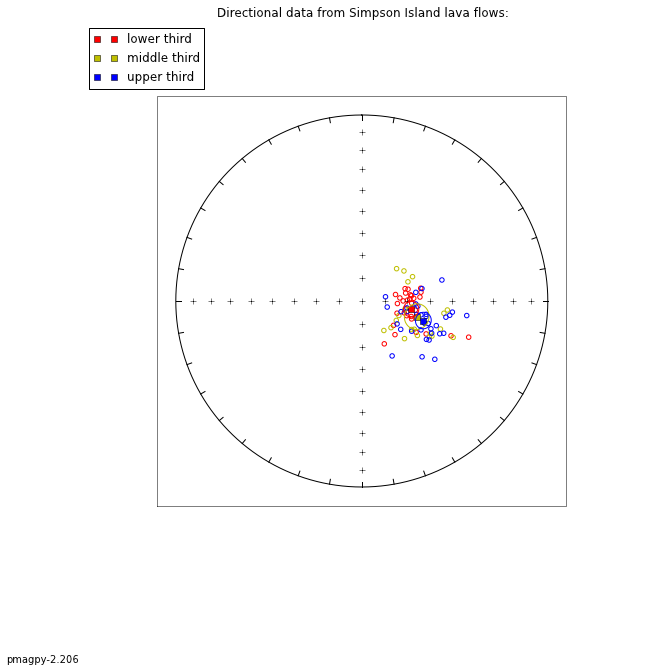
\includegraphics[max size={\textwidth}{\textheight}]{2014_Osler_Data_Analysis_files/2014_Osler_Data_Analysis_15_1.png}
    \par
    \end{center}
    
            \end{InvisibleVerbatim}
            
        
    
\subsection{Test for a common mean between paleomagnetic data from the lower, middle
and upper thirds of the stratigraphy}The code below will compare the subsets of data using:

\begin{enumerate}
\def\labelenumi{\arabic{enumi}.}
\itemsep1pt\parskip0pt\parsep0pt
\item
  The $V_w$ test of Watson (1983) slightly modified from the
  implementation of PmagPy (Tauxe, 2013). The test is comprised of
  calculating the $V_w$ statistic for the two data sets and then
  determining the critical value of $V_w$ through a Monte Carlo
  simulation. For the simulation, two Fisher-distributed data sets with
  a common mean are simulated using the $k_1$ and $k_2$ precisions and
  the $N_1$ and $N_2$ number of points of the datasets being evaluated.
  Then the $V_w$ statistic that comes from comparison between the two
  simulated data sets is calculated. A large number of simulations are
  done (default is 1000; it can be set as the NumSims parameter of the
  function) in order to determine the $V_w$ values that would result by
  chance through sampling distributions with the same direction. The
  critical value of $V_w$ is at the 95\% level of confidence (i.e.~if
  1000 $V_w$ values are simulated, it is the 950th one).
\item
  The bootstrap fold test of Tauxe (developed by Tauxe et al., 1991 and
  implemented per Tauxe (2010)). This approach determines the cumulative
  distributions of the Cartesian coordinates of bootstrapped means and
  compares the cumulative distributions to see if the confidence
  intervals overlap. If they do all overlap, then the two means cannot
  be distinguished at the 95\% level of confidence and they pass the
  bootstrap test for a common mean. Otherwise, if the two sets of
  directions are distinct in the X, Y or Z component the two means can
  be distinguished at the 95\% confidence level.
\end{enumerate}\subsubsection{Common mean tests between SI\_LowerThird\_Directions and
SI\_MiddleThird\_Directions:}

    % Make sure that atleast 4 lines are below the HR
    \needspace{4\baselineskip}

    
        \vspace{6pt}
        \makebox[0.1\linewidth]{\smaller\hfill\tt\color{nbframe-in-prompt}In\hspace{4pt}{[}6{]}:\hspace{4pt}}\\*
        \vspace{-2.65\baselineskip}
        \begin{ColorVerbatim}
            \vspace{-0.7\baselineskip}
            \begin{Verbatim}[commandchars=\\\{\}]
\PY{n}{IPmag}\PY{o}{.}\PY{n}{iWatsonV}\PY{p}{(}\PY{n}{SI\PYZus{}LowerThird\PYZus{}Directions}\PY{p}{,}\PY{n}{SI\PYZus{}MiddleThird\PYZus{}Directions}\PY{p}{)}
\PY{n}{IPmag}\PY{o}{.}\PY{n}{iBootstrap}\PY{p}{(}\PY{n}{SI\PYZus{}LowerThird\PYZus{}Directions}\PY{p}{,}\PY{n}{SI\PYZus{}MiddleThird\PYZus{}Directions}\PY{p}{)}
\end{Verbatim}

            
                \vspace{-0.2\baselineskip}
            
        \end{ColorVerbatim}
    

    

        % If the first block is an image, minipage the image.  Else
        % request a certain amount of space for the input text.
        \needspace{4\baselineskip}
        
        

            % Add document contents.
            
                \begin{InvisibleVerbatim}
                \vspace{-0.5\baselineskip}
\begin{alltt}Results of Watson V test:

Watson's V:           2.6
Critical value of V:  6.3
"Pass": Since V is less than Vcrit, the null hypothesis
that the two populations are drawn from distributions
that share a common mean direction can not be rejected.

M\&M1990 classification:

Angle between data set means: 4.1
Critical angle for M\&M1990:   6.4
The McFadden and McElhinny (1990) classification for
this test is: 'B'

===============

Here are the results of the bootstrap test for a common mean
\end{alltt}

            \end{InvisibleVerbatim}
            
                \begin{InvisibleVerbatim}
                \vspace{-0.5\baselineskip}
    \begin{center}
    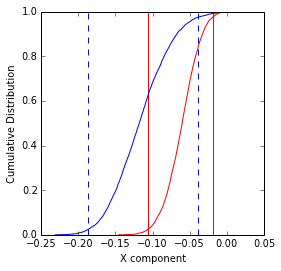
\includegraphics[max size={\textwidth}{\textheight}]{2014_Osler_Data_Analysis_files/2014_Osler_Data_Analysis_19_1.png}
    \par
    \end{center}
    
            \end{InvisibleVerbatim}
            
                \begin{InvisibleVerbatim}
                \vspace{-0.5\baselineskip}
    \begin{center}
    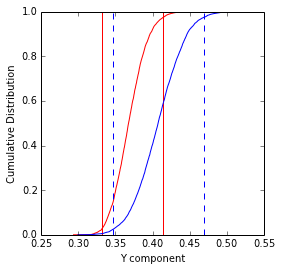
\includegraphics[max size={\textwidth}{\textheight}]{2014_Osler_Data_Analysis_files/2014_Osler_Data_Analysis_19_2.png}
    \par
    \end{center}
    
            \end{InvisibleVerbatim}
            
                \begin{InvisibleVerbatim}
                \vspace{-0.5\baselineskip}
    \begin{center}
    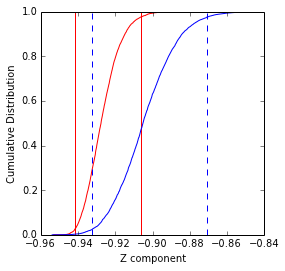
\includegraphics[max size={\textwidth}{\textheight}]{2014_Osler_Data_Analysis_files/2014_Osler_Data_Analysis_19_3.png}
    \par
    \end{center}
    
            \end{InvisibleVerbatim}
            
        
    
\subsubsection{Common mean tests between SI\_MiddleThird\_Directions and
SI\_UpperThird\_Directions:}

    % Make sure that atleast 4 lines are below the HR
    \needspace{4\baselineskip}

    
        \vspace{6pt}
        \makebox[0.1\linewidth]{\smaller\hfill\tt\color{nbframe-in-prompt}In\hspace{4pt}{[}7{]}:\hspace{4pt}}\\*
        \vspace{-2.65\baselineskip}
        \begin{ColorVerbatim}
            \vspace{-0.7\baselineskip}
            \begin{Verbatim}[commandchars=\\\{\}]
\PY{n}{IPmag}\PY{o}{.}\PY{n}{iWatsonV}\PY{p}{(}\PY{n}{SI\PYZus{}MiddleThird\PYZus{}Directions}\PY{p}{,}\PY{n}{SI\PYZus{}UpperThird\PYZus{}Directions}\PY{p}{)}
\PY{n}{IPmag}\PY{o}{.}\PY{n}{iBootstrap}\PY{p}{(}\PY{n}{SI\PYZus{}MiddleThird\PYZus{}Directions}\PY{p}{,}\PY{n}{SI\PYZus{}UpperThird\PYZus{}Directions}\PY{p}{)}
\end{Verbatim}

            
                \vspace{-0.2\baselineskip}
            
        \end{ColorVerbatim}
    

    

        % If the first block is an image, minipage the image.  Else
        % request a certain amount of space for the input text.
        \needspace{4\baselineskip}
        
        

            % Add document contents.
            
                \begin{InvisibleVerbatim}
                \vspace{-0.5\baselineskip}
\begin{alltt}Results of Watson V test:

Watson's V:           1.8
Critical value of V:  6.1
"Pass": Since V is less than Vcrit, the null hypothesis
that the two populations are drawn from distributions
that share a common mean direction can not be rejected.

M\&M1990 classification:

Angle between data set means: 3.4
Critical angle for M\&M1990:   6.4
The McFadden and McElhinny (1990) classification for
this test is: 'B'

===============

Here are the results of the bootstrap test for a common mean
\end{alltt}

            \end{InvisibleVerbatim}
            
                \begin{InvisibleVerbatim}
                \vspace{-0.5\baselineskip}
    \begin{center}
    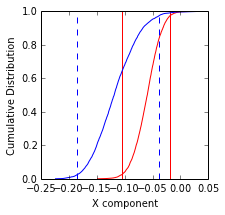
\includegraphics[max size={\textwidth}{\textheight}]{2014_Osler_Data_Analysis_files/2014_Osler_Data_Analysis_21_1.png}
    \par
    \end{center}
    
            \end{InvisibleVerbatim}
            
                \begin{InvisibleVerbatim}
                \vspace{-0.5\baselineskip}
    \begin{center}
    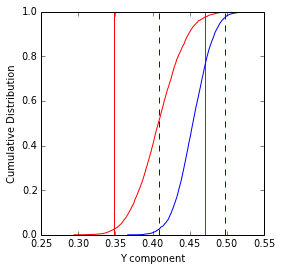
\includegraphics[max size={\textwidth}{\textheight}]{2014_Osler_Data_Analysis_files/2014_Osler_Data_Analysis_21_2.png}
    \par
    \end{center}
    
            \end{InvisibleVerbatim}
            
                \begin{InvisibleVerbatim}
                \vspace{-0.5\baselineskip}
    \begin{center}
    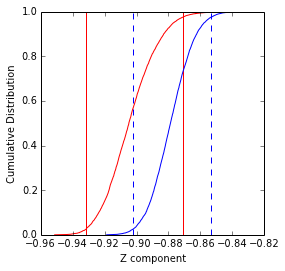
\includegraphics[max size={\textwidth}{\textheight}]{2014_Osler_Data_Analysis_files/2014_Osler_Data_Analysis_21_3.png}
    \par
    \end{center}
    
            \end{InvisibleVerbatim}
            
        
    
\subsubsection{Common mean tests between SI\_LowerThird\_Directions and
SI\_UpperThird\_Directions:}

    % Make sure that atleast 4 lines are below the HR
    \needspace{4\baselineskip}

    
        \vspace{6pt}
        \makebox[0.1\linewidth]{\smaller\hfill\tt\color{nbframe-in-prompt}In\hspace{4pt}{[}8{]}:\hspace{4pt}}\\*
        \vspace{-2.65\baselineskip}
        \begin{ColorVerbatim}
            \vspace{-0.7\baselineskip}
            \begin{Verbatim}[commandchars=\\\{\}]
\PY{n}{IPmag}\PY{o}{.}\PY{n}{iWatsonV}\PY{p}{(}\PY{n}{SI\PYZus{}LowerThird\PYZus{}Directions}\PY{p}{,}\PY{n}{SI\PYZus{}UpperThird\PYZus{}Directions}\PY{p}{)}
\PY{n}{IPmag}\PY{o}{.}\PY{n}{iBootstrap}\PY{p}{(}\PY{n}{SI\PYZus{}LowerThird\PYZus{}Directions}\PY{p}{,}\PY{n}{SI\PYZus{}UpperThird\PYZus{}Directions}\PY{p}{)}
\end{Verbatim}

            
                \vspace{-0.2\baselineskip}
            
        \end{ColorVerbatim}
    

    

        % If the first block is an image, minipage the image.  Else
        % request a certain amount of space for the input text.
        \needspace{4\baselineskip}
        
        

            % Add document contents.
            
                \begin{InvisibleVerbatim}
                \vspace{-0.5\baselineskip}
\begin{alltt}Results of Watson V test:

Watson's V:           14.5
Critical value of V:  6.4
"Fail": Since V is greater than Vcrit, the two means can
be distinguished at the 95\% confidence level.

M\&M1990 classification:

Angle between data set means: 7.4
Critical angle for M\&M1990:   4.9


===============

Here are the results of the bootstrap test for a common mean
\end{alltt}

            \end{InvisibleVerbatim}
            
                \begin{InvisibleVerbatim}
                \vspace{-0.5\baselineskip}
    \begin{center}
    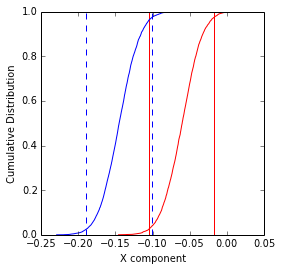
\includegraphics[max size={\textwidth}{\textheight}]{2014_Osler_Data_Analysis_files/2014_Osler_Data_Analysis_23_1.png}
    \par
    \end{center}
    
            \end{InvisibleVerbatim}
            
                \begin{InvisibleVerbatim}
                \vspace{-0.5\baselineskip}
    \begin{center}
    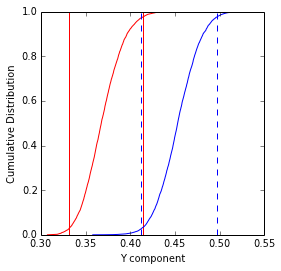
\includegraphics[max size={\textwidth}{\textheight}]{2014_Osler_Data_Analysis_files/2014_Osler_Data_Analysis_23_2.png}
    \par
    \end{center}
    
            \end{InvisibleVerbatim}
            
                \begin{InvisibleVerbatim}
                \vspace{-0.5\baselineskip}
    \begin{center}
    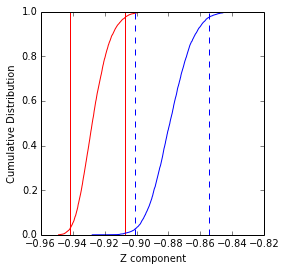
\includegraphics[max size={\textwidth}{\textheight}]{2014_Osler_Data_Analysis_files/2014_Osler_Data_Analysis_23_3.png}
    \par
    \end{center}
    
            \end{InvisibleVerbatim}
            
        
    
The above results from common mean statistical tests show that the
directions from the lower third cannot be distinguished as being
obtained from a distribution distinct from that of the middle third nor
can the directions from the upper third be distinguished from those of
the middle third. In contrast, directions from the lower third of the
stratigraphy can be distinguished from those of upper third at the 95\%
confidence level.\subsection{Plotting the data stratigraphically}Using the flow means calculated for each portion of the stratigraphy,
the paleolatitude and 95\% confidence bounds on paleolatitude can be
calculated. The stratigraphic bounds (y-axis error bars) and
paleolatitude bounds (x-axis error bars) are displayed for points
plotted in the middle of the stratigraphic bin and at the mean
paleolatitude.

    % Make sure that atleast 4 lines are below the HR
    \needspace{4\baselineskip}

    
        \vspace{6pt}
        \makebox[0.1\linewidth]{\smaller\hfill\tt\color{nbframe-in-prompt}In\hspace{4pt}{[}9{]}:\hspace{4pt}}\\*
        \vspace{-2.65\baselineskip}
        \begin{ColorVerbatim}
            \vspace{-0.7\baselineskip}
            \begin{Verbatim}[commandchars=\\\{\}]
\PY{n}{SI\PYZus{}LowerThird\PYZus{}plat}\PY{o}{=}\PY{n}{numpy}\PY{o}{.}\PY{n}{abs}\PY{p}{(}\PY{n}{IPmag}\PY{o}{.}\PY{n}{lat\PYZus{}from\PYZus{}i}\PY{p}{(}\PY{n}{SI\PYZus{}LowerThird\PYZus{}mean}\PY{p}{[}\PY{l+m+mi}{1}\PY{p}{]}\PY{p}{)}\PY{p}{)}
\PY{n}{SI\PYZus{}LowerThird\PYZus{}plat\PYZus{}max}\PY{o}{=}\PY{n}{numpy}\PY{o}{.}\PY{n}{abs}\PY{p}{(}\PY{n}{IPmag}\PY{o}{.}\PY{n}{lat\PYZus{}from\PYZus{}i}\PY{p}{(}\PY{n}{SI\PYZus{}LowerThird\PYZus{}mean}\PY{p}{[}\PY{l+m+mi}{1}\PY{p}{]}\PY{o}{\PYZhy{}}
                                                   \PY{n}{SI\PYZus{}LowerThird\PYZus{}mean}\PY{p}{[}\PY{l+m+mi}{2}\PY{p}{]}\PY{p}{)}\PY{p}{)}
\PY{n}{SI\PYZus{}LowerThird\PYZus{}plat\PYZus{}min}\PY{o}{=}\PY{n}{numpy}\PY{o}{.}\PY{n}{abs}\PY{p}{(}\PY{n}{IPmag}\PY{o}{.}\PY{n}{lat\PYZus{}from\PYZus{}i}\PY{p}{(}\PY{n}{SI\PYZus{}LowerThird\PYZus{}mean}\PY{p}{[}\PY{l+m+mi}{1}\PY{p}{]}\PY{o}{+}
                                                   \PY{n}{SI\PYZus{}LowerThird\PYZus{}mean}\PY{p}{[}\PY{l+m+mi}{2}\PY{p}{]}\PY{p}{)}\PY{p}{)}

\PY{n}{SI\PYZus{}MiddleThird\PYZus{}plat}\PY{o}{=}\PY{n}{numpy}\PY{o}{.}\PY{n}{abs}\PY{p}{(}\PY{n}{IPmag}\PY{o}{.}\PY{n}{lat\PYZus{}from\PYZus{}i}\PY{p}{(}\PY{n}{SI\PYZus{}MiddleThird\PYZus{}mean}\PY{p}{[}\PY{l+m+mi}{1}\PY{p}{]}\PY{p}{)}\PY{p}{)}
\PY{n}{SI\PYZus{}MiddleThird\PYZus{}plat\PYZus{}max}\PY{o}{=}\PY{n}{numpy}\PY{o}{.}\PY{n}{abs}\PY{p}{(}\PY{n}{IPmag}\PY{o}{.}\PY{n}{lat\PYZus{}from\PYZus{}i}\PY{p}{(}\PY{n}{SI\PYZus{}MiddleThird\PYZus{}mean}\PY{p}{[}\PY{l+m+mi}{1}\PY{p}{]}\PY{o}{\PYZhy{}}
                                                    \PY{n}{SI\PYZus{}MiddleThird\PYZus{}mean}\PY{p}{[}\PY{l+m+mi}{2}\PY{p}{]}\PY{p}{)}\PY{p}{)}
\PY{n}{SI\PYZus{}MiddleThird\PYZus{}plat\PYZus{}min}\PY{o}{=}\PY{n}{numpy}\PY{o}{.}\PY{n}{abs}\PY{p}{(}\PY{n}{IPmag}\PY{o}{.}\PY{n}{lat\PYZus{}from\PYZus{}i}\PY{p}{(}\PY{n}{SI\PYZus{}MiddleThird\PYZus{}mean}\PY{p}{[}\PY{l+m+mi}{1}\PY{p}{]}\PY{o}{+}
                                                    \PY{n}{SI\PYZus{}MiddleThird\PYZus{}mean}\PY{p}{[}\PY{l+m+mi}{2}\PY{p}{]}\PY{p}{)}\PY{p}{)}

\PY{n}{SI\PYZus{}UpperThird\PYZus{}plat}\PY{o}{=}\PY{n}{numpy}\PY{o}{.}\PY{n}{abs}\PY{p}{(}\PY{n}{IPmag}\PY{o}{.}\PY{n}{lat\PYZus{}from\PYZus{}i}\PY{p}{(}\PY{n}{SI\PYZus{}UpperThird\PYZus{}mean}\PY{p}{[}\PY{l+m+mi}{1}\PY{p}{]}\PY{p}{)}\PY{p}{)}
\PY{n}{SI\PYZus{}UpperThird\PYZus{}plat\PYZus{}max}\PY{o}{=}\PY{n}{numpy}\PY{o}{.}\PY{n}{abs}\PY{p}{(}\PY{n}{IPmag}\PY{o}{.}\PY{n}{lat\PYZus{}from\PYZus{}i}\PY{p}{(}\PY{n}{SI\PYZus{}UpperThird\PYZus{}mean}\PY{p}{[}\PY{l+m+mi}{1}\PY{p}{]}\PY{o}{\PYZhy{}}
                                                   \PY{n}{SI\PYZus{}UpperThird\PYZus{}mean}\PY{p}{[}\PY{l+m+mi}{2}\PY{p}{]}\PY{p}{)}\PY{p}{)}
\PY{n}{SI\PYZus{}UpperThird\PYZus{}plat\PYZus{}min}\PY{o}{=}\PY{n}{numpy}\PY{o}{.}\PY{n}{abs}\PY{p}{(}\PY{n}{IPmag}\PY{o}{.}\PY{n}{lat\PYZus{}from\PYZus{}i}\PY{p}{(}\PY{n}{SI\PYZus{}UpperThird\PYZus{}mean}\PY{p}{[}\PY{l+m+mi}{1}\PY{p}{]}\PY{o}{+}
                                                   \PY{n}{SI\PYZus{}UpperThird\PYZus{}mean}\PY{p}{[}\PY{l+m+mi}{2}\PY{p}{]}\PY{p}{)}\PY{p}{)}

\PY{n}{SI\PYZus{}LowerThird\PYZus{}meanstrat}\PY{o}{=}\PY{l+m+mi}{521}
\PY{n}{SI\PYZus{}MiddleThird\PYZus{}meanstrat}\PY{o}{=}\PY{l+m+mi}{521}\PY{o}{+}\PY{l+m+mi}{1041}
\PY{n}{SI\PYZus{}UpperThird\PYZus{}meanstrat}\PY{o}{=}\PY{l+m+mi}{521}\PY{o}{+}\PY{l+m+mi}{1041}\PY{o}{+}\PY{l+m+mi}{1041}

\PY{n}{figure}\PY{p}{(}\PY{p}{)}
\PY{n}{errorbar}\PY{p}{(}\PY{n}{SI\PYZus{}LowerThird\PYZus{}plat}\PY{p}{,} \PY{n}{SI\PYZus{}LowerThird\PYZus{}meanstrat}\PY{p}{,} \PY{n}{yerr}\PY{o}{=}\PY{p}{[}\PY{p}{[}\PY{l+m+mi}{521}\PY{p}{]}\PY{p}{,}\PY{p}{[}\PY{l+m+mi}{521}\PY{p}{]}\PY{p}{]}\PY{p}{,}
         \PY{n}{xerr}\PY{o}{=}\PY{p}{[}\PY{p}{[}\PY{n}{SI\PYZus{}LowerThird\PYZus{}plat}\PY{o}{\PYZhy{}}\PY{n}{SI\PYZus{}LowerThird\PYZus{}plat\PYZus{}min}\PY{p}{]}\PY{p}{,}
               \PY{p}{[}\PY{n}{SI\PYZus{}LowerThird\PYZus{}plat\PYZus{}max}\PY{o}{\PYZhy{}}\PY{n}{SI\PYZus{}LowerThird\PYZus{}plat}\PY{p}{]}\PY{p}{]}\PY{p}{,} 
         \PY{n}{fmt}\PY{o}{=}\PY{l+s}{\PYZsq{}}\PY{l+s}{ro}\PY{l+s}{\PYZsq{}}\PY{p}{,}\PY{n}{label}\PY{o}{=}\PY{l+s}{\PYZdq{}}\PY{l+s}{lower third (N=30)}\PY{l+s}{\PYZdq{}}\PY{p}{)}
\PY{n}{errorbar}\PY{p}{(}\PY{n}{SI\PYZus{}MiddleThird\PYZus{}plat}\PY{p}{,} \PY{n}{SI\PYZus{}MiddleThird\PYZus{}meanstrat}\PY{p}{,} \PY{n}{yerr}\PY{o}{=}\PY{p}{[}\PY{p}{[}\PY{l+m+mi}{521}\PY{p}{]}\PY{p}{,}\PY{p}{[}\PY{l+m+mi}{521}\PY{p}{]}\PY{p}{]}\PY{p}{,}
         \PY{n}{xerr}\PY{o}{=}\PY{p}{[}\PY{p}{[}\PY{n}{SI\PYZus{}MiddleThird\PYZus{}plat}\PY{o}{\PYZhy{}}\PY{n}{SI\PYZus{}MiddleThird\PYZus{}plat\PYZus{}min}\PY{p}{]}\PY{p}{,}
               \PY{p}{[}\PY{n}{SI\PYZus{}MiddleThird\PYZus{}plat\PYZus{}max}\PY{o}{\PYZhy{}}\PY{n}{SI\PYZus{}MiddleThird\PYZus{}plat}\PY{p}{]}\PY{p}{]}\PY{p}{,}
         \PY{n}{fmt}\PY{o}{=}\PY{l+s}{\PYZsq{}}\PY{l+s}{yo}\PY{l+s}{\PYZsq{}}\PY{p}{,}\PY{n}{label}\PY{o}{=}\PY{l+s}{\PYZdq{}}\PY{l+s}{middle third (N=20)}\PY{l+s}{\PYZdq{}}\PY{p}{)}
\PY{n}{errorbar}\PY{p}{(}\PY{n}{SI\PYZus{}UpperThird\PYZus{}plat}\PY{p}{,} \PY{n}{SI\PYZus{}UpperThird\PYZus{}meanstrat}\PY{p}{,} \PY{n}{yerr}\PY{o}{=}\PY{p}{[}\PY{p}{[}\PY{l+m+mi}{521}\PY{p}{]}\PY{p}{,}\PY{p}{[}\PY{l+m+mi}{521}\PY{p}{]}\PY{p}{]}\PY{p}{,}
         \PY{n}{xerr}\PY{o}{=}\PY{p}{[}\PY{p}{[}\PY{n}{SI\PYZus{}UpperThird\PYZus{}plat}\PY{o}{\PYZhy{}}\PY{n}{SI\PYZus{}UpperThird\PYZus{}plat\PYZus{}min}\PY{p}{]}\PY{p}{,}
               \PY{p}{[}\PY{n}{SI\PYZus{}UpperThird\PYZus{}plat\PYZus{}max}\PY{o}{\PYZhy{}}\PY{n}{SI\PYZus{}UpperThird\PYZus{}plat}\PY{p}{]}\PY{p}{]}\PY{p}{,}
         \PY{n}{fmt}\PY{o}{=}\PY{l+s}{\PYZsq{}}\PY{l+s}{bo}\PY{l+s}{\PYZsq{}}\PY{p}{,}\PY{n}{label}\PY{o}{=}\PY{l+s}{\PYZdq{}}\PY{l+s}{upper third (N=34)}\PY{l+s}{\PYZdq{}}\PY{p}{)}
\PY{n}{xlabel}\PY{p}{(}\PY{l+s}{\PYZsq{}}\PY{l+s}{paleolatitude (degrees)}\PY{l+s}{\PYZsq{}}\PY{p}{)}
\PY{n}{ylabel}\PY{p}{(}\PY{l+s}{\PYZsq{}}\PY{l+s}{stratigraphic thickness (meters)}\PY{l+s}{\PYZsq{}}\PY{p}{)}
\PY{n}{legend}\PY{p}{(}\PY{n}{bbox\PYZus{}to\PYZus{}anchor}\PY{o}{=}\PY{p}{(}\PY{l+m+mf}{1.05}\PY{p}{,} \PY{l+m+mi}{1}\PY{p}{)}\PY{p}{,} \PY{n}{loc}\PY{o}{=}\PY{l+m+mi}{2}\PY{p}{,} \PY{n}{borderaxespad}\PY{o}{=}\PY{l+m+mf}{0.}\PY{p}{)}
\PY{n}{fig} \PY{o}{=} \PY{n}{matplotlib}\PY{o}{.}\PY{n}{pyplot}\PY{o}{.}\PY{n}{gcf}\PY{p}{(}\PY{p}{)}
\PY{n}{fig}\PY{o}{.}\PY{n}{set\PYZus{}size\PYZus{}inches}\PY{p}{(}\PY{l+m+mi}{5}\PY{p}{,}\PY{l+m+mi}{10}\PY{p}{)}
\PY{n}{pylab}\PY{o}{.}\PY{n}{xlim}\PY{p}{(}\PY{p}{[}\PY{l+m+mi}{20}\PY{p}{,}\PY{l+m+mi}{70}\PY{p}{]}\PY{p}{)}
\PY{n}{pylab}\PY{o}{.}\PY{n}{ylim}\PY{p}{(}\PY{p}{[}\PY{l+m+mi}{0}\PY{p}{,}\PY{l+m+mi}{3200}\PY{p}{]}\PY{p}{)}
\PY{n}{plt}\PY{o}{.}\PY{n}{show}\PY{p}{(}\PY{p}{)}
\end{Verbatim}

            
                \vspace{-0.2\baselineskip}
            
        \end{ColorVerbatim}
    

    

        % If the first block is an image, minipage the image.  Else
        % request a certain amount of space for the input text.
        \needspace{4\baselineskip}
        
        

            % Add document contents.
            
                \begin{InvisibleVerbatim}
                \vspace{-0.5\baselineskip}
    \begin{center}
    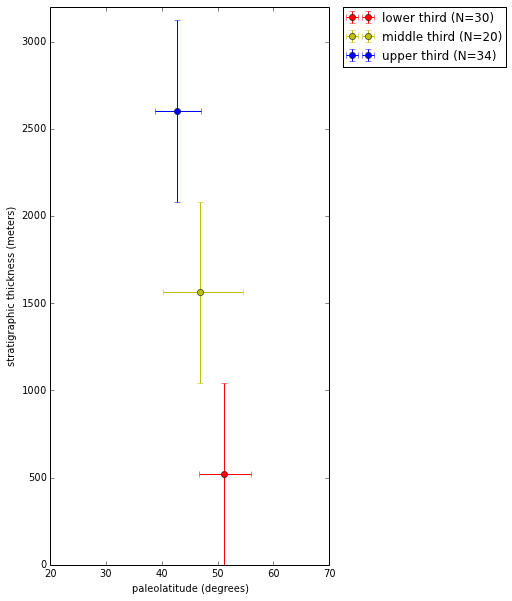
\includegraphics[max size={\textwidth}{\textheight}]{2014_Osler_Data_Analysis_files/2014_Osler_Data_Analysis_27_0.png}
    \par
    \end{center}
    
            \end{InvisibleVerbatim}
            
        
    
\section{Comparing larger and smaller stratigraphic subsets of the Simpson Island
data}\subsection{Comparing data from the lowermost 500 meters to data from the uppermost
500 meters}The analysis above demonstrates that the directions from the lower third
of the stratigraphy (0 to 1041 meters; 30 flows) and the upper third of
the stratigraphy (2083 to 3124 meters; 34 flows) are statistically
distinct and thus indicate statistically significant motion to lower
latitudes. While it is preferable to have a high total number of flows
for such comparisons in order to average out secular variation, let's
conduct this same analysis but for an even more restricted range from
the bottom 500 meters (17 flows) and top 500 meters (17 flows) of the
stratigraphy.

    % Make sure that atleast 4 lines are below the HR
    \needspace{4\baselineskip}

    
        \vspace{6pt}
        \makebox[0.1\linewidth]{\smaller\hfill\tt\color{nbframe-in-prompt}In\hspace{4pt}{[}10{]}:\hspace{4pt}}\\*
        \vspace{-2.65\baselineskip}
        \begin{ColorVerbatim}
            \vspace{-0.7\baselineskip}
            \begin{Verbatim}[commandchars=\\\{\}]
\PY{n}{SI\PYZus{}Lower500m\PYZus{}Directions}\PY{o}{=}\PY{n}{SI\PYZus{}Directions}\PY{p}{[}\PY{l+m+mi}{0}\PY{p}{:}\PY{l+m+mi}{17}\PY{p}{]}
\PY{n}{SI\PYZus{}Lower500m\PYZus{}Poles}\PY{o}{=}\PY{n}{SI\PYZus{}Poles}\PY{p}{[}\PY{l+m+mi}{0}\PY{p}{:}\PY{l+m+mi}{17}\PY{p}{]}
    
\PY{n}{SI\PYZus{}Upper500m\PYZus{}Directions}\PY{o}{=}\PY{n}{SI\PYZus{}Directions}\PY{p}{[}\PY{l+m+mi}{67}\PY{p}{:}\PY{l+m+mi}{84}\PY{p}{]}
\PY{n}{SI\PYZus{}Upper500m\PYZus{}Poles}\PY{o}{=}\PY{n}{SI\PYZus{}Poles}\PY{p}{[}\PY{l+m+mi}{67}\PY{p}{:}\PY{l+m+mi}{84}\PY{p}{]}
    
\PY{n}{pars\PYZus{}1}\PY{o}{=}\PY{n}{pmag}\PY{o}{.}\PY{n}{fisher\PYZus{}mean}\PY{p}{(}\PY{n}{SI\PYZus{}Lower500m\PYZus{}Directions}\PY{p}{)}
\PY{n}{pars\PYZus{}2}\PY{o}{=}\PY{n}{pmag}\PY{o}{.}\PY{n}{fisher\PYZus{}mean}\PY{p}{(}\PY{n}{SI\PYZus{}Upper500m\PYZus{}Directions}\PY{p}{)}

\PY{k}{print} \PY{l+s}{\PYZsq{}}\PY{l+s}{The fisher mean parameters for SI\PYZus{}Lower500m\PYZus{}Directions are: }\PY{l+s}{\PYZsq{}}
\PY{k}{print} \PY{n+nb}{str}\PY{p}{(}\PY{n}{pars\PYZus{}1}\PY{p}{)}
\PY{k}{print} \PY{l+s}{\PYZsq{}}\PY{l+s}{\PYZsq{}}
\PY{k}{print} \PY{l+s}{\PYZsq{}}\PY{l+s}{The fisher mean parameters for SI\PYZus{}Upper500m\PYZus{}Directions are: }\PY{l+s}{\PYZsq{}}
\PY{k}{print} \PY{n+nb}{str}\PY{p}{(}\PY{n}{pars\PYZus{}2}\PY{p}{)}
\end{Verbatim}

            
                \vspace{-0.2\baselineskip}
            
        \end{ColorVerbatim}
    

    

        % If the first block is an image, minipage the image.  Else
        % request a certain amount of space for the input text.
        \needspace{4\baselineskip}
        
        

            % Add document contents.
            
                \begin{InvisibleVerbatim}
                \vspace{-0.5\baselineskip}
\begin{alltt}The fisher mean parameters for SI\_Lower500m\_Directions are:
\{'csd': 6.1620447880184264, 'k': 172.79068906699587, 'n': 17, 'r':
16.907402417998366, 'alpha95': 2.7213037577811798, 'dec':
89.559211694218391, 'inc': -69.03709846618041\}

The fisher mean parameters for SI\_Upper500m\_Directions are:
\{'csd': 10.397718441452353, 'k': 60.686757213380318, 'n': 17, 'r':
16.736351047004497, 'alpha95': 4.6160969512802765, 'dec':
106.9155955500684, 'inc': -56.37171406134344\}
\end{alltt}

            \end{InvisibleVerbatim}
            
        
    


    % Make sure that atleast 4 lines are below the HR
    \needspace{4\baselineskip}

    
        \vspace{6pt}
        \makebox[0.1\linewidth]{\smaller\hfill\tt\color{nbframe-in-prompt}In\hspace{4pt}{[}11{]}:\hspace{4pt}}\\*
        \vspace{-2.65\baselineskip}
        \begin{ColorVerbatim}
            \vspace{-0.7\baselineskip}
            \begin{Verbatim}[commandchars=\\\{\}]
\PY{n}{IPmag}\PY{o}{.}\PY{n}{iWatsonV}\PY{p}{(}\PY{n}{SI\PYZus{}Lower500m\PYZus{}Directions}\PY{p}{,}\PY{n}{SI\PYZus{}Upper500m\PYZus{}Directions}\PY{p}{)}
\PY{n}{IPmag}\PY{o}{.}\PY{n}{iBootstrap}\PY{p}{(}\PY{n}{SI\PYZus{}Lower500m\PYZus{}Directions}\PY{p}{,}\PY{n}{SI\PYZus{}Upper500m\PYZus{}Directions}\PY{p}{)}
\end{Verbatim}

            
                \vspace{-0.2\baselineskip}
            
        \end{ColorVerbatim}
    

    

        % If the first block is an image, minipage the image.  Else
        % request a certain amount of space for the input text.
        \needspace{4\baselineskip}
        
        

            % Add document contents.
            
                \begin{InvisibleVerbatim}
                \vspace{-0.5\baselineskip}
\begin{alltt}Results of Watson V test:

Watson's V:           50.4
Critical value of V:  6.7
"Fail": Since V is greater than Vcrit, the two means can
be distinguished at the 95\% confidence level.

M\&M1990 classification:

Angle between data set means: 14.8
Critical angle for M\&M1990:   5.4


===============

Here are the results of the bootstrap test for a common mean
\end{alltt}

            \end{InvisibleVerbatim}
            
                \begin{InvisibleVerbatim}
                \vspace{-0.5\baselineskip}
    \begin{center}
    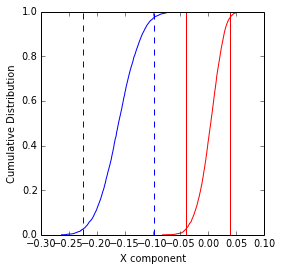
\includegraphics[max size={\textwidth}{\textheight}]{2014_Osler_Data_Analysis_files/2014_Osler_Data_Analysis_32_1.png}
    \par
    \end{center}
    
            \end{InvisibleVerbatim}
            
                \begin{InvisibleVerbatim}
                \vspace{-0.5\baselineskip}
    \begin{center}
    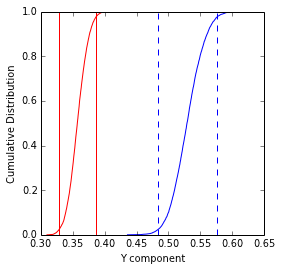
\includegraphics[max size={\textwidth}{\textheight}]{2014_Osler_Data_Analysis_files/2014_Osler_Data_Analysis_32_2.png}
    \par
    \end{center}
    
            \end{InvisibleVerbatim}
            
                \begin{InvisibleVerbatim}
                \vspace{-0.5\baselineskip}
    \begin{center}
    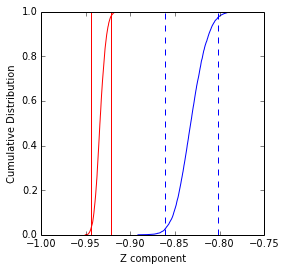
\includegraphics[max size={\textwidth}{\textheight}]{2014_Osler_Data_Analysis_files/2014_Osler_Data_Analysis_32_3.png}
    \par
    \end{center}
    
            \end{InvisibleVerbatim}
            
        
    
The results of this comparision between the lower 500 meters and upper
500 meters show that they are distinct populations at the 95\%
confidence level. The difference between the populations is more
dramatic in both the Watson V and bootstrap test from the tests on the
lower third and upper third subsets that were conducted above. This
increase in difference with tighter stratigraphic groups from lower and
higher in the sequence is the expected result if the sequence is a
record of progressive paleogeographic change.\subsection{Comparison between data from the lower 1/2 and upper 1/2 of Simpson
Island stratigraphy}

    % Make sure that atleast 4 lines are below the HR
    \needspace{4\baselineskip}

    
        \vspace{6pt}
        \makebox[0.1\linewidth]{\smaller\hfill\tt\color{nbframe-in-prompt}In\hspace{4pt}{[}12{]}:\hspace{4pt}}\\*
        \vspace{-2.65\baselineskip}
        \begin{ColorVerbatim}
            \vspace{-0.7\baselineskip}
            \begin{Verbatim}[commandchars=\\\{\}]
\PY{n}{SI\PYZus{}Directions}\PY{o}{=}\PY{p}{[}\PY{p}{]}
\PY{n}{SI\PYZus{}Poles}\PY{o}{=}\PY{p}{[}\PY{p}{]}

\PY{k}{for} \PY{n}{n} \PY{o+ow}{in} \PY{n+nb}{range}\PY{p}{(}\PY{l+m+mi}{0}\PY{p}{,}\PY{l+m+mi}{84}\PY{p}{)}\PY{p}{:}
    \PY{n}{Dec}\PY{p}{,}\PY{n}{Inc}\PY{o}{=}\PY{n}{Dec\PYZus{}TC}\PY{p}{[}\PY{n}{n}\PY{p}{]}\PY{p}{,}\PY{n}{Inc\PYZus{}TC}\PY{p}{[}\PY{n}{n}\PY{p}{]} 
    \PY{n}{SI\PYZus{}Directions}\PY{o}{.}\PY{n}{append}\PY{p}{(}\PY{p}{[}\PY{n}{Dec}\PY{p}{,}\PY{n}{Inc}\PY{p}{,}\PY{l+m+mf}{1.}\PY{p}{]}\PY{p}{)}
    \PY{n}{Plong}\PY{p}{,}\PY{n}{Plat}\PY{o}{=}\PY{n}{VGP\PYZus{}long}\PY{p}{[}\PY{n}{n}\PY{p}{]}\PY{p}{,}\PY{n}{VGP\PYZus{}lat}\PY{p}{[}\PY{n}{n}\PY{p}{]}
    \PY{n}{SI\PYZus{}Poles}\PY{o}{.}\PY{n}{append}\PY{p}{(}\PY{p}{[}\PY{n}{Plong}\PY{p}{,}\PY{n}{Plat}\PY{p}{,}\PY{l+m+mf}{1.}\PY{p}{]}\PY{p}{)}
    
\PY{n}{SI\PYZus{}LowerHalf\PYZus{}Directions}\PY{o}{=}\PY{n}{SI\PYZus{}Directions}\PY{p}{[}\PY{l+m+mi}{0}\PY{p}{:}\PY{l+m+mi}{41}\PY{p}{]}
\PY{n}{SI\PYZus{}LowerHalf\PYZus{}Poles}\PY{o}{=}\PY{n}{SI\PYZus{}Poles}\PY{p}{[}\PY{l+m+mi}{0}\PY{p}{:}\PY{l+m+mi}{41}\PY{p}{]}
\PY{n}{SI\PYZus{}UpperHalf\PYZus{}Directions}\PY{o}{=}\PY{n}{SI\PYZus{}Directions}\PY{p}{[}\PY{l+m+mi}{41}\PY{p}{:}\PY{l+m+mi}{84}\PY{p}{]}
\PY{n}{SI\PYZus{}UpperHalf\PYZus{}Poles}\PY{o}{=}\PY{n}{SI\PYZus{}Poles}\PY{p}{[}\PY{l+m+mi}{41}\PY{p}{:}\PY{l+m+mi}{84}\PY{p}{]}
 
\PY{n}{pars\PYZus{}1}\PY{o}{=}\PY{n}{pmag}\PY{o}{.}\PY{n}{fisher\PYZus{}mean}\PY{p}{(}\PY{n}{SI\PYZus{}LowerHalf\PYZus{}Directions}\PY{p}{)}
\PY{n}{pars\PYZus{}2}\PY{o}{=}\PY{n}{pmag}\PY{o}{.}\PY{n}{fisher\PYZus{}mean}\PY{p}{(}\PY{n}{SI\PYZus{}UpperHalf\PYZus{}Directions}\PY{p}{)}

\PY{k}{print} \PY{l+s}{\PYZsq{}}\PY{l+s}{The fisher mean parameters for SI\PYZus{}LowerHalf\PYZus{}Directions are: }\PY{l+s}{\PYZsq{}} 
\PY{k}{print} \PY{n+nb}{str}\PY{p}{(}\PY{n}{pars\PYZus{}1}\PY{p}{)}
\PY{k}{print} \PY{l+s}{\PYZsq{}}\PY{l+s}{\PYZsq{}}
\PY{k}{print} \PY{l+s}{\PYZsq{}}\PY{l+s}{The fisher mean parameters for SI\PYZus{}UpperHalf\PYZus{}Directions are: }\PY{l+s}{\PYZsq{}}
\PY{k}{print} \PY{n+nb}{str}\PY{p}{(}\PY{n}{pars\PYZus{}2}\PY{p}{)}

\PY{n}{IPmag}\PY{o}{.}\PY{n}{iWatsonV}\PY{p}{(}\PY{n}{SI\PYZus{}LowerHalf\PYZus{}Directions}\PY{p}{,}\PY{n}{SI\PYZus{}UpperHalf\PYZus{}Directions}\PY{p}{)}
\PY{n}{IPmag}\PY{o}{.}\PY{n}{iBootstrap}\PY{p}{(}\PY{n}{SI\PYZus{}LowerHalf\PYZus{}Directions}\PY{p}{,}\PY{n}{SI\PYZus{}UpperHalf\PYZus{}Directions}\PY{p}{)}
\end{Verbatim}

            
                \vspace{-0.2\baselineskip}
            
        \end{ColorVerbatim}
    

    

        % If the first block is an image, minipage the image.  Else
        % request a certain amount of space for the input text.
        \needspace{4\baselineskip}
        
        

            % Add document contents.
            
                \begin{InvisibleVerbatim}
                \vspace{-0.5\baselineskip}
\begin{alltt}The fisher mean parameters for SI\_LowerHalf\_Directions are:
\{'csd': 11.890992902895112, 'k': 46.401689960333911, 'n': 41, 'r':
40.137962431234861, 'alpha95': 3.3119762971808, 'dec':
98.368399411680969, 'inc': -66.192087927867661\}

The fisher mean parameters for SI\_UpperHalf\_Directions are:
\{'csd': 11.246339102175027, 'k': 51.873755310093365, 'n': 43, 'r':
42.19034201883148, 'alpha95': 3.0524627905260902, 'dec':
109.92657619138177, 'inc': -63.09292348420847\}
Results of Watson V test:

Watson's V:           10.4
Critical value of V:  6.5
"Fail": Since V is greater than Vcrit, the two means can
be distinguished at the 95\% confidence level.

M\&M1990 classification:

Angle between data set means: 5.8
Critical angle for M\&M1990:   4.6


===============

Here are the results of the bootstrap test for a common mean
\end{alltt}

            \end{InvisibleVerbatim}
            
                \begin{InvisibleVerbatim}
                \vspace{-0.5\baselineskip}
    \begin{center}
    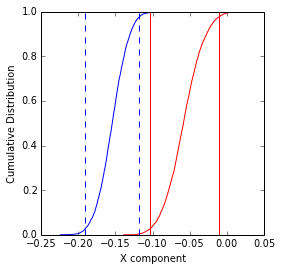
\includegraphics[max size={\textwidth}{\textheight}]{2014_Osler_Data_Analysis_files/2014_Osler_Data_Analysis_35_1.png}
    \par
    \end{center}
    
            \end{InvisibleVerbatim}
            
                \begin{InvisibleVerbatim}
                \vspace{-0.5\baselineskip}
    \begin{center}
    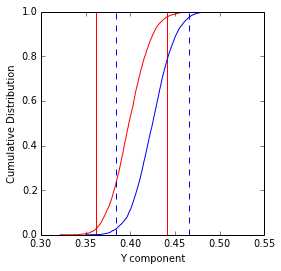
\includegraphics[max size={\textwidth}{\textheight}]{2014_Osler_Data_Analysis_files/2014_Osler_Data_Analysis_35_2.png}
    \par
    \end{center}
    
            \end{InvisibleVerbatim}
            
                \begin{InvisibleVerbatim}
                \vspace{-0.5\baselineskip}
    \begin{center}
    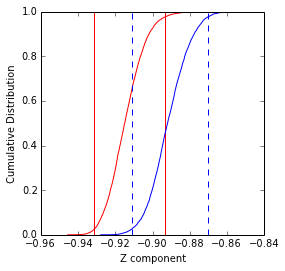
\includegraphics[max size={\textwidth}{\textheight}]{2014_Osler_Data_Analysis_files/2014_Osler_Data_Analysis_35_3.png}
    \par
    \end{center}
    
            \end{InvisibleVerbatim}
            
        
    
\section{Calculating and plotting mean pole positions}\subsection{Loading the basemap library in order to display maps and plot poles.}

    % Make sure that atleast 4 lines are below the HR
    \needspace{4\baselineskip}

    
        \vspace{6pt}
        \makebox[0.1\linewidth]{\smaller\hfill\tt\color{nbframe-in-prompt}In\hspace{4pt}{[}13{]}:\hspace{4pt}}\\*
        \vspace{-2.65\baselineskip}
        \begin{ColorVerbatim}
            \vspace{-0.7\baselineskip}
            \begin{Verbatim}[commandchars=\\\{\}]
\PY{k+kn}{from} \PY{n+nn}{mpl\PYZus{}toolkits.basemap} \PY{k+kn}{import} \PY{n}{Basemap}
\end{Verbatim}

            
                \vspace{-0.2\baselineskip}
            
        \end{ColorVerbatim}
    
The code below calculates the Fisher mean parameters for poles of the
stratigraphically grouped virtual geomagnetic poles (VGPs) and then
plots them on a ``view from space'' globe.

    % Make sure that atleast 4 lines are below the HR
    \needspace{4\baselineskip}

    
        \vspace{6pt}
        \makebox[0.1\linewidth]{\smaller\hfill\tt\color{nbframe-in-prompt}In\hspace{4pt}{[}14{]}:\hspace{4pt}}\\*
        \vspace{-2.65\baselineskip}
        \begin{ColorVerbatim}
            \vspace{-0.7\baselineskip}
            \begin{Verbatim}[commandchars=\\\{\}]
\PY{n}{pars\PYZus{}1}\PY{o}{=}\PY{n}{pmag}\PY{o}{.}\PY{n}{fisher\PYZus{}mean}\PY{p}{(}\PY{n}{SI\PYZus{}LowerThird\PYZus{}Poles}\PY{p}{)}
\PY{n}{pars\PYZus{}2}\PY{o}{=}\PY{n}{pmag}\PY{o}{.}\PY{n}{fisher\PYZus{}mean}\PY{p}{(}\PY{n}{SI\PYZus{}MiddleThird\PYZus{}Poles}\PY{p}{)}
\PY{n}{pars\PYZus{}3}\PY{o}{=}\PY{n}{pmag}\PY{o}{.}\PY{n}{fisher\PYZus{}mean}\PY{p}{(}\PY{n}{SI\PYZus{}UpperThird\PYZus{}Poles}\PY{p}{)}

\PY{k}{print} \PY{l+s}{\PYZsq{}}\PY{l+s}{The fisher mean parameters for SI\PYZus{}LowerThird\PYZus{}Poles are: }\PY{l+s}{\PYZsq{}}
\PY{k}{print} \PY{n+nb}{str}\PY{p}{(}\PY{n}{pars\PYZus{}1}\PY{p}{)}
\PY{k}{print} \PY{l+s}{\PYZsq{}}\PY{l+s}{\PYZsq{}}
\PY{k}{print} \PY{l+s}{\PYZsq{}}\PY{l+s}{The fisher mean parameters for SI\PYZus{}MiddleThird\PYZus{}Poles are: }\PY{l+s}{\PYZsq{}} 
\PY{k}{print} \PY{n+nb}{str}\PY{p}{(}\PY{n}{pars\PYZus{}2}\PY{p}{)}
\PY{k}{print} \PY{l+s}{\PYZsq{}}\PY{l+s}{\PYZsq{}}
\PY{k}{print} \PY{l+s}{\PYZsq{}}\PY{l+s}{The fisher mean parameters for SI\PYZus{}UpperThird\PYZus{}Poles are: }\PY{l+s}{\PYZsq{}}
\PY{k}{print} \PY{n+nb}{str}\PY{p}{(}\PY{n}{pars\PYZus{}3}\PY{p}{)}

\PY{n}{figure}\PY{p}{(}\PY{n}{figsize}\PY{o}{=}\PY{p}{(}\PY{l+m+mi}{8}\PY{p}{,} \PY{l+m+mi}{8}\PY{p}{)}\PY{p}{)}
\PY{n}{m} \PY{o}{=} \PY{n}{Basemap}\PY{p}{(}\PY{n}{projection}\PY{o}{=}\PY{l+s}{\PYZsq{}}\PY{l+s}{ortho}\PY{l+s}{\PYZsq{}}\PY{p}{,}\PY{n}{lat\PYZus{}0}\PY{o}{=}\PY{l+m+mi}{35}\PY{p}{,}\PY{n}{lon\PYZus{}0}\PY{o}{=}\PY{l+m+mi}{200}\PY{p}{,}\PY{n}{resolution}\PY{o}{=}\PY{l+s}{\PYZsq{}}\PY{l+s}{l}\PY{l+s}{\PYZsq{}}\PY{p}{)}
\PY{c}{\PYZsh{} draw coastlines, country boundaries, fill continents.}
\PY{n}{m}\PY{o}{.}\PY{n}{drawcoastlines}\PY{p}{(}\PY{n}{linewidth}\PY{o}{=}\PY{l+m+mf}{0.25}\PY{p}{)}
\PY{c}{\PYZsh{}map.drawcountries(linewidth=0.25)}
\PY{n}{m}\PY{o}{.}\PY{n}{fillcontinents}\PY{p}{(}\PY{n}{color}\PY{o}{=}\PY{l+s}{\PYZsq{}}\PY{l+s}{coral}\PY{l+s}{\PYZsq{}}\PY{p}{,}\PY{n}{lake\PYZus{}color}\PY{o}{=}\PY{l+s}{\PYZsq{}}\PY{l+s}{white}\PY{l+s}{\PYZsq{}}\PY{p}{)}
\PY{n}{m}\PY{o}{.}\PY{n}{drawmapboundary}\PY{p}{(}\PY{n}{fill\PYZus{}color}\PY{o}{=}\PY{l+s}{\PYZsq{}}\PY{l+s}{white}\PY{l+s}{\PYZsq{}}\PY{p}{)}
\PY{n}{m}\PY{o}{.}\PY{n}{drawmeridians}\PY{p}{(}\PY{n}{np}\PY{o}{.}\PY{n}{arange}\PY{p}{(}\PY{l+m+mi}{0}\PY{p}{,}\PY{l+m+mi}{360}\PY{p}{,}\PY{l+m+mi}{30}\PY{p}{)}\PY{p}{)}
\PY{n}{m}\PY{o}{.}\PY{n}{drawparallels}\PY{p}{(}\PY{n}{np}\PY{o}{.}\PY{n}{arange}\PY{p}{(}\PY{o}{\PYZhy{}}\PY{l+m+mi}{90}\PY{p}{,}\PY{l+m+mi}{90}\PY{p}{,}\PY{l+m+mi}{30}\PY{p}{)}\PY{p}{)}

\PY{n}{plong}\PY{p}{,}\PY{n}{plat}\PY{o}{=}\PY{n}{pars\PYZus{}1}\PY{p}{[}\PY{l+s}{\PYZsq{}}\PY{l+s}{dec}\PY{l+s}{\PYZsq{}}\PY{p}{]}\PY{p}{,}\PY{n}{pars\PYZus{}1}\PY{p}{[}\PY{l+s}{\PYZsq{}}\PY{l+s}{inc}\PY{l+s}{\PYZsq{}}\PY{p}{]}
\PY{n}{centerlon}\PY{p}{,} \PY{n}{centerlat} \PY{o}{=} \PY{n}{m}\PY{p}{(}\PY{n}{plong}\PY{p}{,}\PY{n}{plat}\PY{p}{)}
\PY{n}{A95}\PY{o}{=}\PY{n}{pars\PYZus{}1}\PY{p}{[}\PY{l+s}{\PYZsq{}}\PY{l+s}{alpha95}\PY{l+s}{\PYZsq{}}\PY{p}{]}
\PY{n}{A95\PYZus{}km}\PY{o}{=}\PY{n}{A95}\PY{o}{*}\PY{l+m+mf}{111.32}
\PY{c}{\PYZsh{} compute native map projection coordinates of lat/lon grid.}
\PY{n}{m}\PY{o}{.}\PY{n}{scatter}\PY{p}{(}\PY{n}{centerlon}\PY{p}{,}\PY{n}{centerlat}\PY{p}{,}\PY{l+m+mi}{10}\PY{p}{,}\PY{n}{marker}\PY{o}{=}\PY{l+s}{\PYZsq{}}\PY{l+s}{o}\PY{l+s}{\PYZsq{}}\PY{p}{,}\PY{n}{color}\PY{o}{=}\PY{l+s}{\PYZsq{}}\PY{l+s}{r}\PY{l+s}{\PYZsq{}}\PY{p}{,}
          \PY{n}{label}\PY{o}{=}\PY{l+s}{\PYZsq{}}\PY{l+s}{Osler Group Lower Reversed Pole}\PY{l+s}{\PYZsq{}}\PY{p}{)}
\PY{n}{IPmag}\PY{o}{.}\PY{n}{equi}\PY{p}{(}\PY{n}{m}\PY{p}{,} \PY{n}{plong}\PY{p}{,} \PY{n}{plat}\PY{p}{,} \PY{n}{A95\PYZus{}km}\PY{p}{,}\PY{l+s}{\PYZsq{}}\PY{l+s}{r}\PY{l+s}{\PYZsq{}}\PY{p}{)}

\PY{n}{plong}\PY{p}{,}\PY{n}{plat}\PY{o}{=}\PY{n}{pars\PYZus{}2}\PY{p}{[}\PY{l+s}{\PYZsq{}}\PY{l+s}{dec}\PY{l+s}{\PYZsq{}}\PY{p}{]}\PY{p}{,}\PY{n}{pars\PYZus{}2}\PY{p}{[}\PY{l+s}{\PYZsq{}}\PY{l+s}{inc}\PY{l+s}{\PYZsq{}}\PY{p}{]}
\PY{n}{centerlon}\PY{p}{,} \PY{n}{centerlat} \PY{o}{=} \PY{n}{m}\PY{p}{(}\PY{n}{plong}\PY{p}{,}\PY{n}{plat}\PY{p}{)}
\PY{n}{A95}\PY{o}{=}\PY{n}{pars\PYZus{}2}\PY{p}{[}\PY{l+s}{\PYZsq{}}\PY{l+s}{alpha95}\PY{l+s}{\PYZsq{}}\PY{p}{]}
\PY{n}{A95\PYZus{}km}\PY{o}{=}\PY{n}{A95}\PY{o}{*}\PY{l+m+mf}{111.32}
\PY{c}{\PYZsh{} compute native map projection coordinates of lat/lon grid.}
\PY{n}{m}\PY{o}{.}\PY{n}{scatter}\PY{p}{(}\PY{n}{centerlon}\PY{p}{,}\PY{n}{centerlat}\PY{p}{,}\PY{l+m+mi}{10}\PY{p}{,}\PY{n}{marker}\PY{o}{=}\PY{l+s}{\PYZsq{}}\PY{l+s}{o}\PY{l+s}{\PYZsq{}}\PY{p}{,}\PY{n}{color}\PY{o}{=}\PY{l+s}{\PYZsq{}}\PY{l+s}{y}\PY{l+s}{\PYZsq{}}\PY{p}{,}
          \PY{n}{label}\PY{o}{=}\PY{l+s}{\PYZsq{}}\PY{l+s}{Osler Group Middle Reversed Pole}\PY{l+s}{\PYZsq{}}\PY{p}{)}
\PY{n}{IPmag}\PY{o}{.}\PY{n}{equi}\PY{p}{(}\PY{n}{m}\PY{p}{,} \PY{n}{plong}\PY{p}{,} \PY{n}{plat}\PY{p}{,} \PY{n}{A95\PYZus{}km}\PY{p}{,}\PY{l+s}{\PYZsq{}}\PY{l+s}{y}\PY{l+s}{\PYZsq{}}\PY{p}{)}

\PY{n}{plong}\PY{p}{,}\PY{n}{plat}\PY{o}{=}\PY{n}{pars\PYZus{}3}\PY{p}{[}\PY{l+s}{\PYZsq{}}\PY{l+s}{dec}\PY{l+s}{\PYZsq{}}\PY{p}{]}\PY{p}{,}\PY{n}{pars\PYZus{}3}\PY{p}{[}\PY{l+s}{\PYZsq{}}\PY{l+s}{inc}\PY{l+s}{\PYZsq{}}\PY{p}{]}
\PY{n}{centerlon}\PY{p}{,} \PY{n}{centerlat} \PY{o}{=} \PY{n}{m}\PY{p}{(}\PY{n}{plong}\PY{p}{,}\PY{n}{plat}\PY{p}{)}
\PY{n}{A95}\PY{o}{=}\PY{n}{pars\PYZus{}3}\PY{p}{[}\PY{l+s}{\PYZsq{}}\PY{l+s}{alpha95}\PY{l+s}{\PYZsq{}}\PY{p}{]}
\PY{n}{A95\PYZus{}km}\PY{o}{=}\PY{n}{A95}\PY{o}{*}\PY{l+m+mf}{111.32}
\PY{c}{\PYZsh{} compute native map projection coordinates of lat/lon grid.}
\PY{n}{m}\PY{o}{.}\PY{n}{scatter}\PY{p}{(}\PY{n}{centerlon}\PY{p}{,}\PY{n}{centerlat}\PY{p}{,}\PY{l+m+mi}{10}\PY{p}{,}\PY{n}{marker}\PY{o}{=}\PY{l+s}{\PYZsq{}}\PY{l+s}{o}\PY{l+s}{\PYZsq{}}\PY{p}{,}\PY{n}{color}\PY{o}{=}\PY{l+s}{\PYZsq{}}\PY{l+s}{b}\PY{l+s}{\PYZsq{}}\PY{p}{,}
          \PY{n}{label}\PY{o}{=}\PY{l+s}{\PYZsq{}}\PY{l+s}{Osler Group Upper Reversed Pole}\PY{l+s}{\PYZsq{}}\PY{p}{)}
\PY{n}{IPmag}\PY{o}{.}\PY{n}{equi}\PY{p}{(}\PY{n}{m}\PY{p}{,} \PY{n}{plong}\PY{p}{,} \PY{n}{plat}\PY{p}{,} \PY{n}{A95\PYZus{}km}\PY{p}{,}\PY{l+s}{\PYZsq{}}\PY{l+s}{b}\PY{l+s}{\PYZsq{}}\PY{p}{)}

\PY{n}{legend}\PY{p}{(}\PY{n}{bbox\PYZus{}to\PYZus{}anchor}\PY{o}{=}\PY{p}{(}\PY{l+m+mf}{1.05}\PY{p}{,} \PY{l+m+mi}{1}\PY{p}{)}\PY{p}{,} \PY{n}{loc}\PY{o}{=}\PY{l+m+mi}{2}\PY{p}{,} \PY{n}{borderaxespad}\PY{o}{=}\PY{l+m+mf}{0.}\PY{p}{)}
\PY{n}{plt}\PY{o}{.}\PY{n}{show}\PY{p}{(}\PY{p}{)}
\end{Verbatim}

            
                \vspace{-0.2\baselineskip}
            
        \end{ColorVerbatim}
    

    

        % If the first block is an image, minipage the image.  Else
        % request a certain amount of space for the input text.
        \needspace{4\baselineskip}
        
        

            % Add document contents.
            
                \begin{InvisibleVerbatim}
                \vspace{-0.5\baselineskip}
\begin{alltt}The fisher mean parameters for SI\_LowerThird\_Poles are:
\{'csd': 14.439647148676523, 'k': 31.467111290778522, 'n': 30, 'r':
29.078402852679442, 'alpha95': 4.7600623203905919, 'dec':
218.63783260894792, 'inc': 40.93731854099876\}

The fisher mean parameters for SI\_MiddleThird\_Poles are:
\{'csd': 19.701654620387572, 'k': 16.903032828663044, 'n': 20, 'r':
18.875941365517491, 'alpha95': 8.1783359746042343, 'dec':
211.26173612532102, 'inc': 42.737807885172735\}

The fisher mean parameters for SI\_UpperThird\_Poles are:
\{'csd': 15.523618638362732, 'k': 27.226016763674149, 'n': 34, 'r':
32.787924054905098, 'alpha95': 4.8039466857390298, 'dec':
205.41022751277507, 'inc': 41.564576182857046\}
\end{alltt}

            \end{InvisibleVerbatim}
            
                \begin{InvisibleVerbatim}
                \vspace{-0.5\baselineskip}
    \begin{center}
    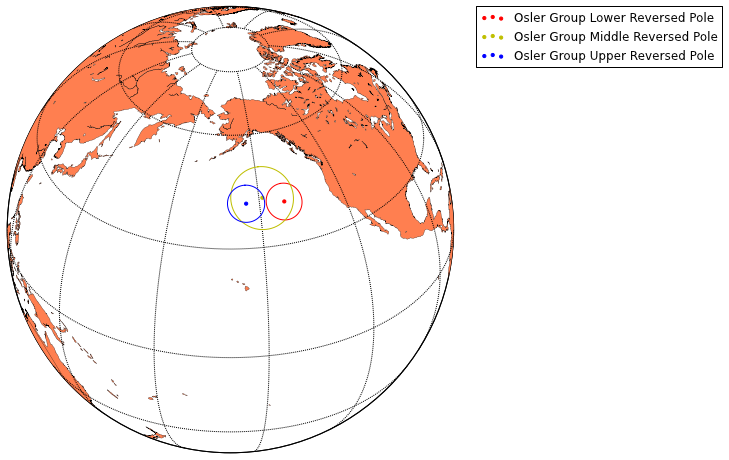
\includegraphics[max size={\textwidth}{\textheight}]{2014_Osler_Data_Analysis_files/2014_Osler_Data_Analysis_40_1.png}
    \par
    \end{center}
    
            \end{InvisibleVerbatim}
            
        
    
Note that in the print out for the mean pole calculations above `dec' is
really the longitude of the pole (Plong) and `inc' is actually the
latitude of the pole (Plat).

Pole ID

Plong

Plat

A95

N

SI\_Lower

218.6

40.9

4.8

30

SI\_Middle

211.3

42.7

8.2

20

SI\_Upper

205.4

41.6

4.8

34\subsection{Comparision between data from Halls (1974) study and Simpson Island VGPs}Halls (1974) developed paleomagnetic data from the Osler Volcanic Group
in the Nipogon Straits region (bibtex citation below; also see
\url{http://earthref.org/MAGIC/9518}). These data are predominantly from
flows with reversed magnetization below an angular unconformity on Puff
Island that seperates the reversedly magnetized flows from younger flows
of normal polarity (only a few of which are preserved before the
sequence is submerged beneath Lake Superior). The analysis below
compares paleomagnetic data from this study with the reversed flows
(N=25) from the Halls (1974) data. The result from this analysis is that
the Halls (1974) data is statistically distinct from the lower third of
the Simpson Island stratigraphy, but is statitically indistinguishable
from the upper third of the Simpson Island stratigraphy. This result
fits with stratigraphic considerations that place the sites studied by
Halls towards the top of the stratigraphy studied herein at Simpson
Island.
%Bibtex citation info for Halls (1974)
@article{Halls1974a,
        Author = {Halls, H.C.},
        Journal = {Canadian Journal of Earth Science},
        Pages = {1200-1207},
        Title = {A paleomagnetic reversal in the {O}sler {V}olcanic
{G}roup, northern {L}ake {S}uperior},
        Volume = {11},
        Year = {1974}}
Import the flow site VGPs from the reversed flows (below the angular
unconformity) of the Halls (1974) study

    % Make sure that atleast 4 lines are below the HR
    \needspace{4\baselineskip}

    
        \vspace{6pt}
        \makebox[0.1\linewidth]{\smaller\hfill\tt\color{nbframe-in-prompt}In\hspace{4pt}{[}15{]}:\hspace{4pt}}\\*
        \vspace{-2.65\baselineskip}
        \begin{ColorVerbatim}
            \vspace{-0.7\baselineskip}
            \begin{Verbatim}[commandchars=\\\{\}]
\PY{n}{OslerHalls\PYZus{}VGP}\PY{o}{=}\PY{p}{[}\PY{p}{]}

\PY{n}{data\PYZus{}file}\PY{o}{=}\PY{l+s}{\PYZsq{}}\PY{l+s}{../2014\PYZus{}Osler\PYZus{}Data/Halls1974\PYZus{}Osler\PYZus{}reversed.csv}\PY{l+s}{\PYZsq{}}
\PY{n}{Halls1974\PYZus{}Osler\PYZus{}reversed} \PY{o}{=} \PY{n}{np}\PY{o}{.}\PY{n}{genfromtxt}\PY{p}{(}\PY{n}{data\PYZus{}file}\PY{p}{,}\PY{n}{delimiter}\PY{o}{=}\PY{l+s}{\PYZdq{}}\PY{l+s}{,}\PY{l+s}{\PYZdq{}}\PY{p}{,} \PY{n}{skip\PYZus{}header}\PY{o}{=}\PY{l+m+mi}{1}\PY{p}{)}

\PY{n}{Halls1974\PYZus{}VGP\PYZus{}long}\PY{o}{=}\PY{n}{Halls1974\PYZus{}Osler\PYZus{}reversed}\PY{p}{[}\PY{p}{:}\PY{p}{,}\PY{l+m+mi}{0}\PY{p}{]}
\PY{n}{Halls1974\PYZus{}VGP\PYZus{}lat}\PY{o}{=}\PY{n}{Halls1974\PYZus{}Osler\PYZus{}reversed}\PY{p}{[}\PY{p}{:}\PY{p}{,}\PY{l+m+mi}{1}\PY{p}{]}

\PY{k}{for} \PY{n}{VGP} \PY{o+ow}{in} \PY{n+nb}{range}\PY{p}{(}\PY{l+m+mi}{0}\PY{p}{,}\PY{n+nb}{len}\PY{p}{(}\PY{n}{Halls1974\PYZus{}VGP\PYZus{}lat}\PY{p}{)}\PY{p}{)}\PY{p}{:}
    \PY{n}{Plong}\PY{p}{,}\PY{n}{Plat}\PY{o}{=}\PY{n}{Halls1974\PYZus{}VGP\PYZus{}long}\PY{p}{[}\PY{n}{VGP}\PY{p}{]}\PY{p}{,}\PY{n}{Halls1974\PYZus{}VGP\PYZus{}lat}\PY{p}{[}\PY{n}{VGP}\PY{p}{]} 
    \PY{n}{OslerHalls\PYZus{}VGP}\PY{o}{.}\PY{n}{append}\PY{p}{(}\PY{p}{[}\PY{n}{Plong}\PY{p}{,}\PY{n}{Plat}\PY{p}{,}\PY{l+m+mf}{1.}\PY{p}{]}\PY{p}{)}
\end{Verbatim}

            
                \vspace{-0.2\baselineskip}
            
        \end{ColorVerbatim}
    
\subsubsection{Common mean tests between Halls (1974) data and the data from the lower
third of the Simpson Island stratigraphy}

    % Make sure that atleast 4 lines are below the HR
    \needspace{4\baselineskip}

    
        \vspace{6pt}
        \makebox[0.1\linewidth]{\smaller\hfill\tt\color{nbframe-in-prompt}In\hspace{4pt}{[}16{]}:\hspace{4pt}}\\*
        \vspace{-2.65\baselineskip}
        \begin{ColorVerbatim}
            \vspace{-0.7\baselineskip}
            \begin{Verbatim}[commandchars=\\\{\}]
\PY{n}{IPmag}\PY{o}{.}\PY{n}{iWatsonV}\PY{p}{(}\PY{n}{OslerHalls\PYZus{}VGP}\PY{p}{,}\PY{n}{SI\PYZus{}LowerThird\PYZus{}Poles}\PY{p}{)}
\PY{n}{IPmag}\PY{o}{.}\PY{n}{iBootstrap}\PY{p}{(}\PY{n}{OslerHalls\PYZus{}VGP}\PY{p}{,}\PY{n}{SI\PYZus{}LowerThird\PYZus{}Poles}\PY{p}{)}
\end{Verbatim}

            
                \vspace{-0.2\baselineskip}
            
        \end{ColorVerbatim}
    

    

        % If the first block is an image, minipage the image.  Else
        % request a certain amount of space for the input text.
        \needspace{4\baselineskip}
        
        

            % Add document contents.
            
                \begin{InvisibleVerbatim}
                \vspace{-0.5\baselineskip}
\begin{alltt}Results of Watson V test:

Watson's V:           31.0
Critical value of V:  6.6
"Fail": Since V is greater than Vcrit, the two means can
be distinguished at the 95\% confidence level.

M\&M1990 classification:

Angle between data set means: 16.7
Critical angle for M\&M1990:   7.7


===============

Here are the results of the bootstrap test for a common mean
\end{alltt}

            \end{InvisibleVerbatim}
            
                \begin{InvisibleVerbatim}
                \vspace{-0.5\baselineskip}
    \begin{center}
    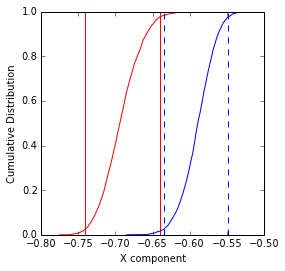
\includegraphics[max size={\textwidth}{\textheight}]{2014_Osler_Data_Analysis_files/2014_Osler_Data_Analysis_48_1.png}
    \par
    \end{center}
    
            \end{InvisibleVerbatim}
            
                \begin{InvisibleVerbatim}
                \vspace{-0.5\baselineskip}
    \begin{center}
    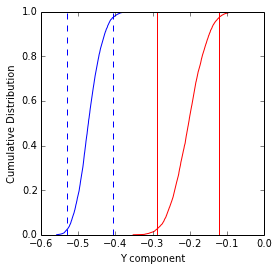
\includegraphics[max size={\textwidth}{\textheight}]{2014_Osler_Data_Analysis_files/2014_Osler_Data_Analysis_48_2.png}
    \par
    \end{center}
    
            \end{InvisibleVerbatim}
            
                \begin{InvisibleVerbatim}
                \vspace{-0.5\baselineskip}
    \begin{center}
    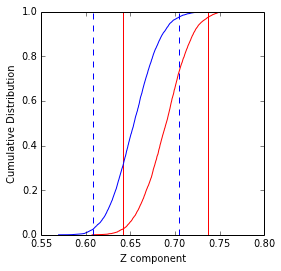
\includegraphics[max size={\textwidth}{\textheight}]{2014_Osler_Data_Analysis_files/2014_Osler_Data_Analysis_48_3.png}
    \par
    \end{center}
    
            \end{InvisibleVerbatim}
            
        
    
A comparision between VGPs calculated from Halls, 1974 data and data
from the lower third of the Simpson Island stratigraphy fails Watson's V
and bootstrap tests for a common mean indicating that the populations of
directions do not share a common mean at the 95\% confidence level.\subsubsection{Common mean tests between Halls (1974) data and the data from the upper
third of the Simpson Island stratigraphy}

    % Make sure that atleast 4 lines are below the HR
    \needspace{4\baselineskip}

    
        \vspace{6pt}
        \makebox[0.1\linewidth]{\smaller\hfill\tt\color{nbframe-in-prompt}In\hspace{4pt}{[}17{]}:\hspace{4pt}}\\*
        \vspace{-2.65\baselineskip}
        \begin{ColorVerbatim}
            \vspace{-0.7\baselineskip}
            \begin{Verbatim}[commandchars=\\\{\}]
\PY{n}{IPmag}\PY{o}{.}\PY{n}{iWatsonV}\PY{p}{(}\PY{n}{OslerHalls\PYZus{}VGP}\PY{p}{,}\PY{n}{SI\PYZus{}UpperThird\PYZus{}Poles}\PY{p}{)}
\PY{n}{IPmag}\PY{o}{.}\PY{n}{iBootstrap}\PY{p}{(}\PY{n}{OslerHalls\PYZus{}VGP}\PY{p}{,}\PY{n}{SI\PYZus{}UpperThird\PYZus{}Poles}\PY{p}{)}
\end{Verbatim}

            
                \vspace{-0.2\baselineskip}
            
        \end{ColorVerbatim}
    

    

        % If the first block is an image, minipage the image.  Else
        % request a certain amount of space for the input text.
        \needspace{4\baselineskip}
        
        

            % Add document contents.
            
                \begin{InvisibleVerbatim}
                \vspace{-0.5\baselineskip}
\begin{alltt}Results of Watson V test:

Watson's V:           5.4
Critical value of V:  7.0
"Pass": Since V is less than Vcrit, the null hypothesis
that the two populations are drawn from distributions
that share a common mean direction can not be rejected.

M\&M1990 classification:

Angle between data set means: 7.0
Critical angle for M\&M1990:   7.9
The McFadden and McElhinny (1990) classification for
this test is: 'B'

===============

Here are the results of the bootstrap test for a common mean
\end{alltt}

            \end{InvisibleVerbatim}
            
                \begin{InvisibleVerbatim}
                \vspace{-0.5\baselineskip}
    \begin{center}
    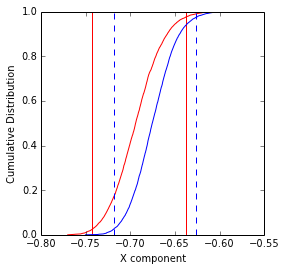
\includegraphics[max size={\textwidth}{\textheight}]{2014_Osler_Data_Analysis_files/2014_Osler_Data_Analysis_51_1.png}
    \par
    \end{center}
    
            \end{InvisibleVerbatim}
            
                \begin{InvisibleVerbatim}
                \vspace{-0.5\baselineskip}
    \begin{center}
    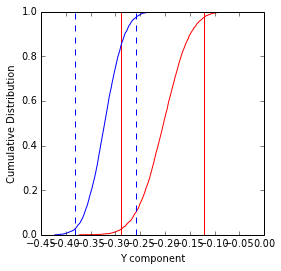
\includegraphics[max size={\textwidth}{\textheight}]{2014_Osler_Data_Analysis_files/2014_Osler_Data_Analysis_51_2.png}
    \par
    \end{center}
    
            \end{InvisibleVerbatim}
            
                \begin{InvisibleVerbatim}
                \vspace{-0.5\baselineskip}
    \begin{center}
    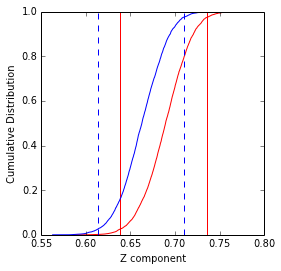
\includegraphics[max size={\textwidth}{\textheight}]{2014_Osler_Data_Analysis_files/2014_Osler_Data_Analysis_51_3.png}
    \par
    \end{center}
    
            \end{InvisibleVerbatim}
            
        
    
A comparision between VGPs calculated from Halls, 1974 data (see
\url{http://earthref.org/MAGIC/9518}) and data from the upper third of
the Simpson Island stratigraphy passes Watson's V and bootstrap tests
for a common mean.\subsubsection{Combining the data from the upper third of the Simpson Island
stratigraphy and the Halls (1974) reversed polarity data into a single
pole for the upper portion of the reversed Osler Group stratigraphy}

    % Make sure that atleast 4 lines are below the HR
    \needspace{4\baselineskip}

    
        \vspace{6pt}
        \makebox[0.1\linewidth]{\smaller\hfill\tt\color{nbframe-in-prompt}In\hspace{4pt}{[}18{]}:\hspace{4pt}}\\*
        \vspace{-2.65\baselineskip}
        \begin{ColorVerbatim}
            \vspace{-0.7\baselineskip}
            \begin{Verbatim}[commandchars=\\\{\}]
\PY{n}{upperR\PYZus{}Osler\PYZus{}VGPs}\PY{o}{=}\PY{n}{OslerHalls\PYZus{}VGP}\PY{o}{+}\PY{n}{SI\PYZus{}UpperThird\PYZus{}Poles}

\PY{n}{pars\PYZus{}1}\PY{o}{=}\PY{n}{pmag}\PY{o}{.}\PY{n}{fisher\PYZus{}mean}\PY{p}{(}\PY{n}{upperR\PYZus{}Osler\PYZus{}VGPs}\PY{p}{)}

\PY{k}{print} \PY{l+s}{\PYZsq{}}\PY{l+s}{The fisher mean parameters for the pole calculated from upper reversed}\PY{l+s}{\PYZsq{}}
\PY{k}{print} \PY{l+s}{\PYZsq{}}\PY{l+s}{Osler Group VGPs (SI\PYZus{}UpperThird\PYZus{}Poles+Halls, 1974 reversed data) are: }\PY{l+s}{\PYZsq{}}
\PY{k}{print} \PY{n+nb}{str}\PY{p}{(}\PY{n}{pars\PYZus{}1}\PY{p}{)}
\end{Verbatim}

            
                \vspace{-0.2\baselineskip}
            
        \end{ColorVerbatim}
    

    

        % If the first block is an image, minipage the image.  Else
        % request a certain amount of space for the input text.
        \needspace{4\baselineskip}
        
        

            % Add document contents.
            
                \begin{InvisibleVerbatim}
                \vspace{-0.5\baselineskip}
\begin{alltt}The fisher mean parameters for the pole calculated from upper reversed
Osler Group VGPs (SI\_UpperThird\_Poles+Halls, 1974 reversed data) are:
\{'csd': 15.984670336321198, 'k': 25.678087233610714, 'n': 59, 'r':
56.741264780653822, 'alpha95': 3.7227743269632096, 'dec':
201.64704637965517, 'inc': 42.537024291694905\}
\end{alltt}

            \end{InvisibleVerbatim}
            
        
    
Pole ID

Plong

Plat

A95

N

approximate age

upper Osler Group reversed pole (this work and Halls, 1974)

201.6

42.5

3.7

59

1105±2 Ma\subsection{Paleogeographic work outside of this IPython notebook using the software
package GPlates.}For details on working with paleomagnetic data in GPlates check out
\href{https://docs.google.com/document/pub?id=1gdgHIaC5WpjLaRZu1JwqotV8zOrgnfu_fZ3aNwQZNmU}{this
tutorial}.

The steps necessary to develop the reconstruction using these Osler
Volcanic Group poles are detailed below.\begin{enumerate}
\def\labelenumi{(\arabic{enumi})}
\itemsep1pt\parskip0pt\parsep0pt
\item
  Develop .rot file that rotates Laurentia such that the Osler poles are
  at geographic north. In the text for the .rot file below the
  Osler\_lowerthird pole is assigned to 1110 Ma, the Osler\_middlethird
  pole is assigned to 1107.5 and the Osler\_upperthird pole is assigned
  to 1105 Ma.
\end{enumerate}

The .rot file has the format:

moving plate ID number

age in millions of years

latitude of Euler pole

longitude of Euler pole

angle

fixed plate

comment

In this .rot file, the fixed reference frame is 000 and 001 (which could
be split into a relative and absolute reference frame that seperates out
TPW), while the plate ID for Laurentia is 199.
001  0.0   0.0    0.0    0.0  000 ! \\
001 3900.0   0.0    0.0    0.0  000 ! \\
199  0.0   0.0    0.0    0.0  001 ! \\
199 1105.0   0.0  115.4   48.4  001 !Put Osler-upperthird at N for
Laurentia \\
199 1107.5   0.0  121.3   47.3  001 !Put Osler-middlethird at N for
Laurentia \\
199 1110.0   0.0  128.7   49.0  001 !Put Osler-lowerthird at N for
Laurentia \\
\begin{enumerate}
\def\labelenumi{(\arabic{enumi})}
\setcounter{enumi}{1}
\itemsep1pt\parskip0pt\parsep0pt
\item
  Open the following feature collections in GPlates: 199-Laurentia
  nogrid.dat, OslerPoles.gpml and Osler.rot where 199-Laurentia
  nogrid.dat is the outline of Laurentia in the late Proterozoic and
  OslerPoles.gpml contains the three calculated Osler paleomagnetic
  poles. An animation from 1110 to 1105 Ma yields the following
  reconstruction shown here with a time slice for Osler\_lowerthird
  (red), Osler\_middlethird (yellow) and Osler\_upperthird (blue).
\end{enumerate}

    % Make sure that atleast 4 lines are below the HR
    \needspace{4\baselineskip}

    
        \vspace{6pt}
        \makebox[0.1\linewidth]{\smaller\hfill\tt\color{nbframe-in-prompt}In\hspace{4pt}{[}19{]}:\hspace{4pt}}\\*
        \vspace{-2.65\baselineskip}
        \begin{ColorVerbatim}
            \vspace{-0.7\baselineskip}
            \begin{Verbatim}[commandchars=\\\{\}]
\PY{k+kn}{from} \PY{n+nn}{IPython.core.display} \PY{k+kn}{import} \PY{n}{SVG}
\PY{n}{Paleogeo}\PY{o}{=}\PY{n}{SVG}\PY{p}{(}\PY{n}{filename}\PY{o}{=}\PY{l+s}{\PYZsq{}}\PY{l+s}{Paleogeo.svg}\PY{l+s}{\PYZsq{}}\PY{p}{)}
\PY{n}{display}\PY{p}{(}\PY{n}{Paleogeo}\PY{p}{)}
\end{Verbatim}

            
                \vspace{-0.2\baselineskip}
            
        \end{ColorVerbatim}
    

    

        % If the first block is an image, minipage the image.  Else
        % request a certain amount of space for the input text.
        \needspace{4\baselineskip}
        
        

            % Add document contents.
            
                \begin{InvisibleVerbatim}
                \vspace{-0.5\baselineskip}
    \begin{center}
    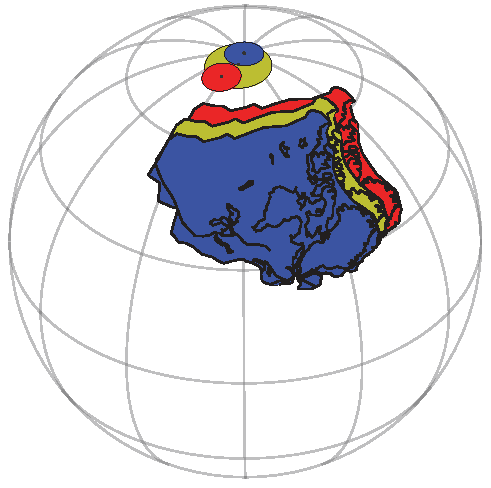
\includegraphics[max size={\textwidth}{\textheight}]{2014_Osler_Data_Analysis_files/2014_Osler_Data_Analysis_61_0.pdf}
    \par
    \end{center}
    
            \end{InvisibleVerbatim}
            
        
    
\section{Lava flow thickness data}In the section of the text entitled ``Osler Volcanic Group lithologies''
the median flow thickness is reported from the subset of flows within
measured sections where there is sufficient exposure of the flow base,
interior and top to determine thickness. In the text it is reported that
the median flow thickness is 4.9 meters with a first quartile thickness
of 2.0 meters and third quartile thickness of 9.8 meters. The flow
thickness data used in this analysis is presented and analyzed below.

    % Make sure that atleast 4 lines are below the HR
    \needspace{4\baselineskip}

    
        \vspace{6pt}
        \makebox[0.1\linewidth]{\smaller\hfill\tt\color{nbframe-in-prompt}In\hspace{4pt}{[}20{]}:\hspace{4pt}}\\*
        \vspace{-2.65\baselineskip}
        \begin{ColorVerbatim}
            \vspace{-0.7\baselineskip}
            \begin{Verbatim}[commandchars=\\\{\}]
\PY{c}{\PYZsh{}flow thicknesses where bottom and top are exposed without cover in between or with minimal cover and assumption of continuity}
\PY{n}{SI1\PYZus{}flowthickness} \PY{o}{=} \PY{n}{array}\PY{p}{(}\PY{p}{[}\PY{l+m+mf}{1.2}\PY{p}{,} \PY{l+m+mf}{1.1}\PY{o}{+}\PY{l+m+mf}{0.7}\PY{p}{,}\PY{l+m+mf}{0.2}\PY{o}{+}\PY{l+m+mf}{2.9}\PY{o}{+}\PY{l+m+mf}{0.3}\PY{p}{,}\PY{l+m+mf}{5.1}\PY{o}{+}\PY{l+m+mf}{5.4}\PY{o}{+}\PY{l+m+mf}{0.6}\PY{o}{+}\PY{l+m+mf}{3.4}\PY{p}{,}\PY{l+m+mf}{0.6}\PY{o}{+}\PY{l+m+mi}{1}\PY{o}{+}\PY{o}{.}\PY{l+m+mi}{3}\PY{p}{,}\PY{l+m+mf}{0.9}\PY{p}{,}\PY{l+m+mf}{0.5}\PY{p}{,}\PY{l+m+mf}{2.2}\PY{p}{,}\PY{l+m+mf}{0.8}\PY{p}{,}\PY{l+m+mf}{0.5}\PY{p}{,}\PY{l+m+mf}{0.3}\PY{o}{+}\PY{l+m+mf}{1.3}\PY{o}{+}\PY{l+m+mf}{0.6}\PY{o}{+}\PY{l+m+mf}{1.6}\PY{p}{,}\PY{l+m+mf}{0.4}\PY{o}{+}\PY{l+m+mf}{2.3}\PY{p}{,}\PY{l+m+mf}{0.6}\PY{p}{,}\PY{l+m+mf}{0.8}\PY{o}{+}\PY{l+m+mf}{1.0}\PY{p}{,}\PY{l+m+mf}{1.6}\PY{o}{+}\PY{l+m+mf}{0.3}\PY{p}{,}\PY{l+m+mf}{1.0}\PY{o}{+}\PY{l+m+mf}{0.6}\PY{o}{+}\PY{l+m+mf}{2.4}\PY{p}{,}\PY{l+m+mf}{0.2}\PY{o}{+}\PY{l+m+mf}{4.4}\PY{o}{+}\PY{l+m+mf}{0.8}\PY{o}{+}\PY{l+m+mf}{0.6}\PY{p}{,}\PY{l+m+mf}{3.3}\PY{o}{+}\PY{l+m+mf}{1.6}\PY{p}{,}\PY{l+m+mf}{0.7}\PY{p}{,}\PY{l+m+mi}{4}\PY{o}{+}\PY{l+m+mf}{4.7}\PY{o}{+}\PY{l+m+mf}{5.7}\PY{o}{+}\PY{l+m+mf}{1.7}\PY{o}{+}\PY{l+m+mf}{1.8}\PY{p}{,}\PY{l+m+mf}{0.9}\PY{p}{,}\PY{l+m+mf}{0.2}\PY{o}{+}\PY{l+m+mf}{0.5}\PY{p}{,}\PY{l+m+mf}{0.2}\PY{o}{+}\PY{l+m+mf}{0.8}\PY{o}{+}\PY{l+m+mf}{1.3}\PY{p}{,}\PY{l+m+mf}{0.2}\PY{o}{+}\PY{l+m+mf}{0.9}\PY{p}{,}\PY{l+m+mf}{1.7}\PY{p}{,}\PY{l+m+mf}{0.6}\PY{p}{,}\PY{l+m+mf}{0.2}\PY{o}{+}\PY{l+m+mf}{1.5}\PY{p}{,}\PY{l+m+mf}{1.2}\PY{o}{+}\PY{l+m+mf}{0.4}\PY{o}{+}\PY{l+m+mf}{1.3}\PY{p}{,}\PY{l+m+mf}{1.3}\PY{o}{+}\PY{l+m+mf}{1.5}\PY{p}{,}\PY{l+m+mf}{1.3}\PY{p}{,}\PY{l+m+mf}{2.4}\PY{p}{,}\PY{l+m+mf}{0.3}\PY{o}{+}\PY{l+m+mf}{1.7}\PY{p}{,}\PY{l+m+mf}{0.6}\PY{o}{+}\PY{l+m+mf}{0.3}\PY{p}{,}\PY{l+m+mf}{0.3}\PY{o}{+}\PY{l+m+mf}{0.5}\PY{o}{+}\PY{o}{.}\PY{l+m+mi}{3}\PY{o}{+}\PY{l+m+mf}{1.3}\PY{p}{,}\PY{l+m+mf}{0.5}\PY{o}{+}\PY{l+m+mf}{1.1}\PY{p}{,}\PY{l+m+mf}{0.1}\PY{o}{+}\PY{l+m+mf}{0.3}\PY{o}{+}\PY{l+m+mf}{1.3}\PY{p}{,}\PY{l+m+mf}{1.5}\PY{p}{,}\PY{l+m+mf}{0.1}\PY{o}{+}\PY{l+m+mf}{1.9}\PY{o}{+}\PY{l+m+mf}{1.7}\PY{o}{+}\PY{l+m+mf}{1.2}\PY{p}{]}\PY{p}{)}
\PY{n}{SI2\PYZus{}flowthickness} \PY{o}{=} \PY{n}{array}\PY{p}{(}\PY{p}{[}\PY{l+m+mf}{0.6}\PY{o}{+}\PY{l+m+mf}{2.8}\PY{p}{,}\PY{l+m+mf}{5.7}\PY{o}{+}\PY{l+m+mi}{2}\PY{o}{+}\PY{l+m+mf}{3.6}\PY{p}{,}\PY{l+m+mf}{1.3}\PY{o}{+}\PY{l+m+mf}{0.7}\PY{o}{+}\PY{l+m+mf}{1.1}\PY{o}{+}\PY{l+m+mf}{1.1}\PY{p}{,}\PY{l+m+mf}{6.2}\PY{o}{+}\PY{l+m+mi}{1}\PY{p}{,}\PY{l+m+mf}{1.8}\PY{o}{+}\PY{l+m+mf}{3.3}\PY{o}{+}\PY{l+m+mf}{11.4}\PY{p}{]}\PY{p}{)}
\PY{n}{SI3\PYZus{}flowthickness} \PY{o}{=} \PY{n}{array}\PY{p}{(}\PY{p}{[}\PY{l+m+mf}{0.6}\PY{o}{+}\PY{l+m+mf}{0.8}\PY{o}{+}\PY{l+m+mi}{1}\PY{o}{+}\PY{o}{.}\PY{l+m+mi}{8}\PY{p}{,}\PY{l+m+mi}{1}\PY{o}{+}\PY{l+m+mf}{4.9}\PY{o}{+}\PY{l+m+mf}{1.1}\PY{p}{,}\PY{l+m+mf}{0.3}\PY{o}{+}\PY{l+m+mf}{1.6}\PY{o}{+}\PY{l+m+mf}{4.5}\PY{o}{+}\PY{l+m+mf}{1.2}\PY{p}{,}\PY{l+m+mf}{0.2}\PY{o}{+}\PY{l+m+mf}{1.5}\PY{o}{+}\PY{l+m+mf}{7.2}\PY{o}{+}\PY{l+m+mf}{0.9}\PY{p}{,}\PY{l+m+mf}{0.5}\PY{o}{+}\PY{l+m+mf}{1.7}\PY{o}{+}\PY{l+m+mf}{9.3}\PY{p}{,}\PY{l+m+mf}{1.4}\PY{o}{+}\PY{l+m+mf}{2.9}\PY{o}{+}\PY{l+m+mf}{0.6}\PY{p}{,}\PY{l+m+mf}{3.1}\PY{o}{+}\PY{l+m+mi}{3}\PY{o}{+}\PY{l+m+mf}{0.9}\PY{p}{,}\PY{l+m+mf}{3.9}\PY{o}{+}\PY{l+m+mf}{1.4}\PY{o}{+}\PY{o}{.}\PY{l+m+mi}{3}\PY{p}{]}\PY{p}{)}
\PY{n}{SI4\PYZus{}flowthickness} \PY{o}{=} \PY{n}{array}\PY{p}{(}\PY{p}{[}\PY{l+m+mf}{0.2}\PY{o}{+}\PY{l+m+mf}{1.2}\PY{o}{+}\PY{l+m+mf}{0.9}\PY{p}{,}\PY{l+m+mf}{0.3}\PY{o}{+}\PY{l+m+mf}{1.5}\PY{o}{+}\PY{l+m+mf}{0.4}\PY{o}{+}\PY{l+m+mf}{3.2}\PY{p}{,}\PY{l+m+mi}{14}\PY{o}{+}\PY{l+m+mf}{6.5}\PY{p}{,}\PY{l+m+mf}{0.7}\PY{o}{+}\PY{l+m+mi}{1}\PY{o}{+}\PY{l+m+mf}{3.6}\PY{p}{,}\PY{l+m+mf}{8.2}\PY{o}{+}\PY{l+m+mf}{2.4}\PY{o}{+}\PY{l+m+mf}{4.6}\PY{p}{,}\PY{l+m+mf}{3.1}\PY{o}{+}\PY{l+m+mf}{1.4}\PY{o}{+}\PY{l+m+mf}{1.4}\PY{p}{,}\PY{l+m+mf}{1.6}\PY{p}{,}\PY{l+m+mf}{2.8}\PY{o}{+}\PY{l+m+mf}{2.1}\PY{p}{,}\PY{l+m+mf}{0.7}\PY{o}{+}\PY{l+m+mf}{5.6}\PY{o}{+}\PY{l+m+mf}{2.4}\PY{o}{+}\PY{l+m+mf}{0.6}\PY{p}{,}\PY{l+m+mf}{5.6}\PY{o}{+}\PY{l+m+mf}{0.7}\PY{p}{,}\PY{l+m+mf}{2.2}\PY{o}{+}\PY{l+m+mf}{0.2}\PY{o}{+}\PY{l+m+mf}{0.3}\PY{p}{,}\PY{l+m+mf}{0.4}\PY{o}{+}\PY{l+m+mf}{2.4}\PY{o}{+}\PY{l+m+mf}{1.9}\PY{o}{+}\PY{l+m+mi}{1}\PY{p}{,}\PY{l+m+mf}{4.2}\PY{o}{+}\PY{l+m+mf}{0.7}\PY{p}{]}\PY{p}{)}
\PY{n}{SI5\PYZus{}flowthickness} \PY{o}{=} \PY{n}{array}\PY{p}{(}\PY{p}{[}\PY{l+m+mf}{6.6}\PY{o}{+}\PY{l+m+mf}{9.8}\PY{o}{+}\PY{l+m+mf}{7.4}\PY{o}{+}\PY{l+m+mf}{1.4}\PY{o}{+}\PY{l+m+mf}{2.3}\PY{p}{,}\PY{l+m+mf}{10.2}\PY{o}{+}\PY{l+m+mf}{0.8}\PY{p}{,}\PY{l+m+mf}{5.6}\PY{o}{+}\PY{l+m+mf}{2.8}\PY{o}{+}\PY{l+m+mf}{1.4}\PY{o}{+}\PY{l+m+mf}{2.2}\PY{p}{,}\PY{l+m+mf}{0.2}\PY{o}{+}\PY{l+m+mf}{2.8}\PY{o}{+}\PY{l+m+mf}{2.4}\PY{o}{+}\PY{l+m+mf}{0.7}\PY{p}{,}\PY{l+m+mf}{0.6}\PY{p}{,}\PY{l+m+mf}{0.2}\PY{o}{+}\PY{l+m+mf}{0.5}\PY{p}{,}\PY{l+m+mf}{0.2}\PY{o}{+}\PY{l+m+mf}{2.2}\PY{p}{,}\PY{l+m+mf}{1.7}\PY{o}{+}\PY{l+m+mf}{1.7}\PY{p}{,}\PY{l+m+mf}{1.6}\PY{o}{+}\PY{l+m+mf}{0.6}\PY{p}{,}\PY{l+m+mf}{0.2}\PY{o}{+}\PY{l+m+mf}{3.8}\PY{o}{+}\PY{l+m+mf}{1.4}\PY{o}{+}\PY{l+m+mi}{1}\PY{p}{,}\PY{l+m+mf}{7.6}\PY{o}{+}\PY{l+m+mf}{20.4}\PY{o}{+}\PY{l+m+mf}{6.3}\PY{o}{+}\PY{l+m+mf}{4.2}\PY{o}{+}\PY{l+m+mi}{1}\PY{p}{,}\PY{l+m+mf}{2.8}\PY{o}{+}\PY{l+m+mf}{1.3}\PY{o}{+}\PY{l+m+mf}{1.2}\PY{p}{,}\PY{l+m+mf}{10.2}\PY{o}{+}\PY{l+m+mi}{9}\PY{p}{]}\PY{p}{)}
\PY{n}{SI6\PYZus{}flowthickness} \PY{o}{=} \PY{n}{array}\PY{p}{(}\PY{p}{[}\PY{l+m+mf}{13.1}\PY{o}{+}\PY{l+m+mf}{3.3}\PY{p}{,}\PY{l+m+mf}{13.5}\PY{o}{+}\PY{l+m+mf}{3.7}\PY{p}{,}\PY{l+m+mf}{6.5}\PY{o}{+}\PY{l+m+mf}{0.6}\PY{p}{,}\PY{l+m+mf}{6.1}\PY{o}{+}\PY{l+m+mf}{2.1}\PY{o}{+}\PY{l+m+mf}{0.9}\PY{p}{,}\PY{l+m+mf}{0.9}\PY{o}{+}\PY{l+m+mf}{6.6}\PY{o}{+}\PY{l+m+mf}{4.0}\PY{p}{,}\PY{l+m+mf}{7.3}\PY{o}{+}\PY{l+m+mf}{5.6}\PY{o}{+}\PY{l+m+mf}{1.3}\PY{o}{+}\PY{l+m+mf}{7.4}\PY{p}{,}\PY{l+m+mf}{0.5}\PY{o}{+}\PY{l+m+mf}{9.6}\PY{o}{+}\PY{l+m+mf}{3.4}\PY{o}{+}\PY{l+m+mf}{0.5}\PY{p}{,}\PY{l+m+mf}{2.8}\PY{o}{+}\PY{l+m+mf}{4.3}\PY{p}{,}\PY{l+m+mf}{0.3}\PY{o}{+}\PY{l+m+mf}{7.4}\PY{o}{+}\PY{l+m+mf}{3.9}\PY{p}{]}\PY{p}{)}
\PY{n}{SI7\PYZus{}flowthickness} \PY{o}{=} \PY{n}{array}\PY{p}{(}\PY{p}{[}\PY{l+m+mf}{0.4}\PY{o}{+}\PY{l+m+mf}{0.9}\PY{o}{+}\PY{l+m+mf}{1.2}\PY{o}{+}\PY{l+m+mf}{1.4}\PY{p}{,}\PY{l+m+mf}{0.3}\PY{o}{+}\PY{l+m+mf}{1.2}\PY{p}{,}\PY{l+m+mf}{0.5}\PY{o}{+}\PY{l+m+mf}{2.5}\PY{o}{+}\PY{l+m+mi}{5}\PY{o}{+}\PY{l+m+mf}{1.9}\PY{p}{]}\PY{p}{)}
\PY{n}{SI8\PYZus{}flowthickness} \PY{o}{=} \PY{n}{array}\PY{p}{(}\PY{p}{[}\PY{l+m+mf}{1.4}\PY{o}{+}\PY{l+m+mf}{1.9}\PY{o}{+}\PY{l+m+mf}{0.6}\PY{p}{,}\PY{l+m+mf}{0.5}\PY{o}{+}\PY{l+m+mi}{1}\PY{o}{+}\PY{l+m+mf}{8.8}\PY{o}{+}\PY{l+m+mi}{4}\PY{o}{+}\PY{l+m+mf}{1.1}\PY{p}{,}\PY{l+m+mi}{5}\PY{o}{+}\PY{l+m+mf}{15.8}\PY{o}{+}\PY{l+m+mf}{2.8}\PY{o}{+}\PY{l+m+mf}{2.1}\PY{p}{,}\PY{l+m+mi}{5}\PY{o}{+}\PY{l+m+mf}{4.2}\PY{p}{,}\PY{l+m+mf}{8.4}\PY{o}{+}\PY{l+m+mf}{8.1}\PY{o}{+}\PY{l+m+mi}{5}\PY{p}{,}\PY{l+m+mf}{1.8}\PY{o}{+}\PY{l+m+mf}{11.8}\PY{o}{+}\PY{l+m+mi}{1}\PY{o}{+}\PY{l+m+mf}{2.2}\PY{o}{+}\PY{l+m+mf}{1.4}\PY{p}{]}\PY{p}{)}
\PY{n}{SI9\PYZus{}flowthickness} \PY{o}{=} \PY{n}{array}\PY{p}{(}\PY{p}{[}\PY{l+m+mf}{5.0}\PY{o}{+}\PY{l+m+mf}{4.2}\PY{p}{,}\PY{l+m+mf}{14.0}\PY{o}{+}\PY{l+m+mi}{1}\PY{o}{+}\PY{l+m+mf}{2.1}\PY{p}{,}\PY{l+m+mf}{2.8}\PY{o}{+}\PY{l+m+mf}{2.1}\PY{p}{,}\PY{l+m+mf}{3.6}\PY{o}{+}\PY{l+m+mf}{12.3}\PY{o}{+}\PY{l+m+mf}{3.6}\PY{o}{+}\PY{l+m+mf}{0.7}\PY{p}{,}\PY{l+m+mf}{4.2}\PY{o}{+}\PY{l+m+mf}{2.3}\PY{p}{,}\PY{l+m+mf}{1.3}\PY{o}{+}\PY{l+m+mf}{1.4}\PY{o}{+}\PY{l+m+mf}{2.2}\PY{p}{,}\PY{l+m+mf}{0.8}\PY{o}{+}\PY{l+m+mf}{1.8}\PY{o}{+}\PY{l+m+mf}{9.8}\PY{o}{+}\PY{l+m+mf}{4.2}\PY{o}{+}\PY{l+m+mf}{0.8}\PY{p}{,}\PY{l+m+mf}{0.2}\PY{o}{+}\PY{l+m+mf}{2.0}\PY{o}{+}\PY{l+m+mf}{0.6}\PY{o}{+}\PY{l+m+mf}{2.3}\PY{p}{,}\PY{l+m+mf}{0.3}\PY{o}{+}\PY{l+m+mf}{0.4}\PY{o}{+}\PY{l+m+mf}{3.3}\PY{p}{,}\PY{l+m+mf}{7.5}\PY{p}{]}\PY{p}{)}
    
\PY{n}{SIall\PYZus{}flowthickness} \PY{o}{=} \PY{n}{concatenate}\PY{p}{(}\PY{p}{(}\PY{n}{SI1\PYZus{}flowthickness}\PY{p}{,} \PY{n}{SI2\PYZus{}flowthickness}\PY{p}{,} 
                                   \PY{n}{SI3\PYZus{}flowthickness}\PY{p}{,} \PY{n}{SI4\PYZus{}flowthickness}\PY{p}{,} 
                                   \PY{n}{SI5\PYZus{}flowthickness}\PY{p}{,} \PY{n}{SI6\PYZus{}flowthickness}\PY{p}{,}
                                   \PY{n}{SI7\PYZus{}flowthickness}\PY{p}{,} \PY{n}{SI8\PYZus{}flowthickness}\PY{p}{,} 
                                   \PY{n}{SI9\PYZus{}flowthickness}\PY{p}{)}\PY{p}{)}
\PY{k}{print} \PY{l+s}{\PYZdq{}}\PY{l+s}{The number of flows for which thickness estimates could be obtained is:}\PY{l+s}{\PYZdq{}}
\PY{k}{print} \PY{n+nb}{len}\PY{p}{(}\PY{n}{SIall\PYZus{}flowthickness}\PY{p}{)}
\PY{k}{print} \PY{l+s}{\PYZdq{}}\PY{l+s}{The mean flow thickness is:}\PY{l+s}{\PYZdq{}}
\PY{k}{print} \PY{n}{mean}\PY{p}{(}\PY{n}{SIall\PYZus{}flowthickness}\PY{p}{)}
\PY{k}{print} \PY{l+s}{\PYZdq{}}\PY{l+s}{The median flow thickness is:}\PY{l+s}{\PYZdq{}}
\PY{k}{print} \PY{n}{median}\PY{p}{(}\PY{n}{SIall\PYZus{}flowthickness}\PY{p}{)}

\PY{k}{print} \PY{l+s}{\PYZdq{}}\PY{l+s}{The first quartile thickness is:}\PY{l+s}{\PYZdq{}}
\PY{k}{print} \PY{n}{percentile}\PY{p}{(}\PY{n}{SIall\PYZus{}flowthickness}\PY{p}{,}\PY{l+m+mi}{25}\PY{p}{)}
\PY{k}{print} \PY{l+s}{\PYZdq{}}\PY{l+s}{The third quartile thickness is:}\PY{l+s}{\PYZdq{}}
\PY{k}{print} \PY{n}{percentile}\PY{p}{(}\PY{n}{SIall\PYZus{}flowthickness}\PY{p}{,}\PY{l+m+mi}{75}\PY{p}{)}

\PY{n}{hist}\PY{p}{(}\PY{n}{SIall\PYZus{}flowthickness}\PY{p}{,} \PY{l+m+mi}{40}\PY{p}{,} \PY{n}{facecolor}\PY{o}{=}\PY{l+s}{\PYZsq{}}\PY{l+s}{green}\PY{l+s}{\PYZsq{}}\PY{p}{)}
\PY{n}{title}\PY{p}{(}\PY{l+s}{\PYZsq{}}\PY{l+s}{Histogram of Osler flow thicknesses within measured sections}\PY{l+s}{\PYZsq{}}\PY{p}{)}
\PY{n}{ylabel}\PY{p}{(}\PY{l+s}{\PYZsq{}}\PY{l+s}{number of flows}\PY{l+s}{\PYZsq{}}\PY{p}{)}
\PY{n}{xlabel}\PY{p}{(}\PY{l+s}{\PYZsq{}}\PY{l+s}{flow thickness (meters)}\PY{l+s}{\PYZsq{}}\PY{p}{)}
\PY{n}{plt}\PY{o}{.}\PY{n}{show}\PY{p}{(}\PY{p}{)}
\PY{n}{data}\PY{o}{=}\PY{p}{(}\PY{n}{SI1\PYZus{}flowthickness}\PY{p}{,}\PY{n}{SI2\PYZus{}flowthickness}\PY{p}{,}\PY{n}{SI3\PYZus{}flowthickness}\PY{p}{,}
      \PY{n}{SI4\PYZus{}flowthickness}\PY{p}{,}\PY{n}{SI5\PYZus{}flowthickness}\PY{p}{,} \PY{n}{SI6\PYZus{}flowthickness}\PY{p}{,}
      \PY{n}{SI7\PYZus{}flowthickness}\PY{p}{,}\PY{n}{SI8\PYZus{}flowthickness}\PY{p}{,}\PY{n}{SI9\PYZus{}flowthickness}\PY{p}{,}\PY{n}{SIall\PYZus{}flowthickness}\PY{p}{)}

\PY{n}{figure}\PY{p}{(}\PY{n}{figsize}\PY{o}{=}\PY{p}{(}\PY{l+m+mi}{12}\PY{p}{,}\PY{l+m+mi}{4}\PY{p}{)}\PY{p}{)}
\PY{n}{title}\PY{p}{(}\PY{l+s}{\PYZsq{}}\PY{l+s}{Boxplot of flow thicknesses grouped by stratigraphic section}\PY{l+s}{\PYZsq{}}\PY{p}{)}
\PY{n}{boxplot}\PY{p}{(}\PY{n}{data}\PY{p}{)}
\PY{n}{labels} \PY{o}{=} \PY{p}{(}\PY{l+s}{\PYZsq{}}\PY{l+s}{SI1}\PY{l+s}{\PYZsq{}}\PY{p}{,} \PY{l+s}{\PYZsq{}}\PY{l+s}{SI2}\PY{l+s}{\PYZsq{}}\PY{p}{,} \PY{l+s}{\PYZsq{}}\PY{l+s}{SI3}\PY{l+s}{\PYZsq{}}\PY{p}{,} \PY{l+s}{\PYZsq{}}\PY{l+s}{SI4}\PY{l+s}{\PYZsq{}}\PY{p}{,} \PY{l+s}{\PYZsq{}}\PY{l+s}{SI5}\PY{l+s}{\PYZsq{}}\PY{p}{,} \PY{l+s}{\PYZsq{}}\PY{l+s}{SI6}\PY{l+s}{\PYZsq{}}\PY{p}{,} 
          \PY{l+s}{\PYZsq{}}\PY{l+s}{SI7}\PY{l+s}{\PYZsq{}}\PY{p}{,} \PY{l+s}{\PYZsq{}}\PY{l+s}{SI8}\PY{l+s}{\PYZsq{}}\PY{p}{,} \PY{l+s}{\PYZsq{}}\PY{l+s}{SI9}\PY{l+s}{\PYZsq{}}\PY{p}{,} \PY{l+s}{\PYZsq{}}\PY{l+s}{all sections}\PY{l+s}{\PYZsq{}}\PY{p}{)}
\PY{n}{xticks}\PY{p}{(}\PY{n+nb}{range}\PY{p}{(}\PY{l+m+mi}{1}\PY{p}{,}\PY{l+m+mi}{11}\PY{p}{)}\PY{p}{,}\PY{n}{labels}\PY{p}{)}
\PY{n}{xlabel}\PY{p}{(}\PY{l+s}{\PYZsq{}}\PY{l+s}{stratigraphic section}\PY{l+s}{\PYZsq{}}\PY{p}{)}
\PY{n}{ylabel}\PY{p}{(}\PY{l+s}{\PYZsq{}}\PY{l+s}{flow thickness (meters)}\PY{l+s}{\PYZsq{}}\PY{p}{)}
\PY{n}{plt}\PY{o}{.}\PY{n}{show}\PY{p}{(}\PY{p}{)}
\end{Verbatim}

            
                \vspace{-0.2\baselineskip}
            
        \end{ColorVerbatim}
    

    

        % If the first block is an image, minipage the image.  Else
        % request a certain amount of space for the input text.
        \needspace{4\baselineskip}
        
        

            % Add document contents.
            
                \begin{InvisibleVerbatim}
                \vspace{-0.5\baselineskip}
\begin{alltt}The number of flows for which thickness estimates could be obtained
is:
105
The mean flow thickness is:
7.16666666667
The median flow thickness is:
4.9
The first quartile thickness is:
2.0
The third quartile thickness is:
9.8
\end{alltt}

            \end{InvisibleVerbatim}
            
                \begin{InvisibleVerbatim}
                \vspace{-0.5\baselineskip}
    \begin{center}
    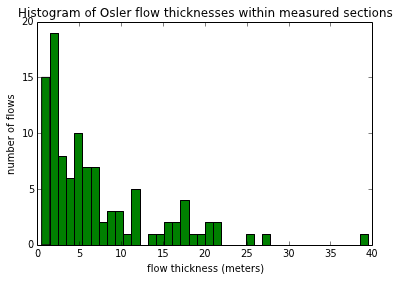
\includegraphics[max size={\textwidth}{\textheight}]{2014_Osler_Data_Analysis_files/2014_Osler_Data_Analysis_64_1.png}
    \par
    \end{center}
    
            \end{InvisibleVerbatim}
            
                \begin{InvisibleVerbatim}
                \vspace{-0.5\baselineskip}
    \begin{center}
    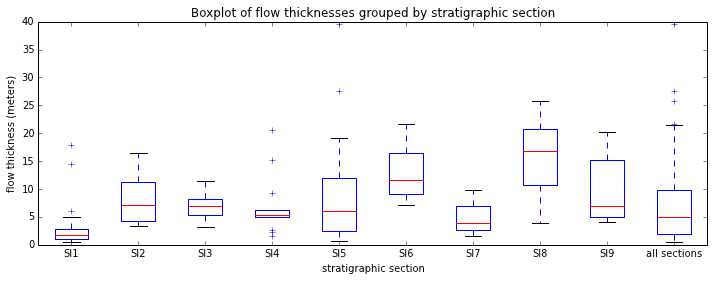
\includegraphics[max size={\textwidth}{\textheight}]{2014_Osler_Data_Analysis_files/2014_Osler_Data_Analysis_64_2.png}
    \par
    \end{center}
    
            \end{InvisibleVerbatim}
            
        
    
\section{The IPmag.py library of functions}Some of the functions used in the analysis above come from the imported
IPmag.py library that was developed for this data analysis project. The
code that is within IPmag.py is shown below so that the PDF output of
this IPython notebook can document more of the tools used in the
analysis without the reader needing to look into the .py file itself.
This library utilizes functions from the pmag.py and pmagplotlib.py
libraries of PmagPy version 2.206.

    % Make sure that atleast 4 lines are below the HR
    \needspace{4\baselineskip}

    
        \vspace{6pt}
        \makebox[0.1\linewidth]{\smaller\hfill\tt\color{nbframe-in-prompt}In\hspace{4pt}{[}21{]}:\hspace{4pt}}\\*
        \vspace{-2.65\baselineskip}
        \begin{ColorVerbatim}
            \vspace{-0.7\baselineskip}
            \begin{Verbatim}[commandchars=\\\{\}]
\PY{k+kn}{import} \PY{n+nn}{pmag}\PY{o}{,} \PY{n+nn}{pmagplotlib}
\PY{k+kn}{import} \PY{n+nn}{pylab}
\PY{k+kn}{import} \PY{n+nn}{numpy}
\PY{k+kn}{import} \PY{n+nn}{matplotlib.pyplot} \PY{k+kn}{as} \PY{n+nn}{plt}

\PY{k}{def} \PY{n+nf}{iplotDI}\PY{p}{(}\PY{n}{DIblock}\PY{p}{,}\PY{n}{color}\PY{o}{=}\PY{l+s}{\PYZsq{}}\PY{l+s}{k}\PY{l+s}{\PYZsq{}}\PY{p}{)}\PY{p}{:}
    \PY{l+s+sd}{\PYZdq{}\PYZdq{}\PYZdq{}}
\PY{l+s+sd}{    Plot declination, inclination data on a equal area plot}

\PY{l+s+sd}{    This function modifies the plotDI function of PmagPy for use in the IPython notebook environment}

\PY{l+s+sd}{    Parameters}
\PY{l+s+sd}{    \PYZhy{}\PYZhy{}\PYZhy{}\PYZhy{}\PYZhy{}\PYZhy{}\PYZhy{}\PYZhy{}\PYZhy{}\PYZhy{}}

\PY{l+s+sd}{    DIblock : a DIblock is comprise of a list of unit vectors [dec,inc,1.]}
\PY{l+s+sd}{    color : the default color is black. Other colors can be chosen (e.g. \PYZsq{}r\PYZsq{})}
\PY{l+s+sd}{    \PYZdq{}\PYZdq{}\PYZdq{}}
    \PY{c}{\PYZsh{} initialize the variables}
    \PY{n}{X\PYZus{}down}\PY{p}{,}\PY{n}{X\PYZus{}up}\PY{p}{,}\PY{n}{Y\PYZus{}down}\PY{p}{,}\PY{n}{Y\PYZus{}up}\PY{o}{=}\PY{p}{[}\PY{p}{]}\PY{p}{,}\PY{p}{[}\PY{p}{]}\PY{p}{,}\PY{p}{[}\PY{p}{]}\PY{p}{,}\PY{p}{[}\PY{p}{]}
    \PY{k}{for} \PY{n}{rec} \PY{o+ow}{in} \PY{n}{DIblock}\PY{p}{:}
        \PY{n}{Up}\PY{p}{,}\PY{n}{Down}\PY{o}{=}\PY{l+m+mi}{0}\PY{p}{,}\PY{l+m+mi}{0}
        \PY{n}{XY}\PY{o}{=}\PY{n}{pmag}\PY{o}{.}\PY{n}{dimap}\PY{p}{(}\PY{n}{rec}\PY{p}{[}\PY{l+m+mi}{0}\PY{p}{]}\PY{p}{,}\PY{n}{rec}\PY{p}{[}\PY{l+m+mi}{1}\PY{p}{]}\PY{p}{)}
        \PY{k}{if} \PY{n}{rec}\PY{p}{[}\PY{l+m+mi}{1}\PY{p}{]} \PY{o}{\PYZgt{}}\PY{o}{=} \PY{l+m+mi}{0}\PY{p}{:}         
            \PY{n}{X\PYZus{}down}\PY{o}{.}\PY{n}{append}\PY{p}{(}\PY{n}{XY}\PY{p}{[}\PY{l+m+mi}{0}\PY{p}{]}\PY{p}{)}
            \PY{n}{Y\PYZus{}down}\PY{o}{.}\PY{n}{append}\PY{p}{(}\PY{n}{XY}\PY{p}{[}\PY{l+m+mi}{1}\PY{p}{]}\PY{p}{)}
        \PY{k}{else}\PY{p}{:}
            \PY{n}{X\PYZus{}up}\PY{o}{.}\PY{n}{append}\PY{p}{(}\PY{n}{XY}\PY{p}{[}\PY{l+m+mi}{0}\PY{p}{]}\PY{p}{)}
            \PY{n}{Y\PYZus{}up}\PY{o}{.}\PY{n}{append}\PY{p}{(}\PY{n}{XY}\PY{p}{[}\PY{l+m+mi}{1}\PY{p}{]}\PY{p}{)}

    \PY{k}{if} \PY{n+nb}{len}\PY{p}{(}\PY{n}{X\PYZus{}up}\PY{p}{)}\PY{o}{\PYZgt{}}\PY{l+m+mi}{0}\PY{p}{:}
        \PY{n}{pylab}\PY{o}{.}\PY{n}{scatter}\PY{p}{(}\PY{n}{X\PYZus{}up}\PY{p}{,}\PY{n}{Y\PYZus{}up}\PY{p}{,}\PY{n}{facecolors}\PY{o}{=}\PY{l+s}{\PYZsq{}}\PY{l+s}{none}\PY{l+s}{\PYZsq{}}\PY{p}{,} \PY{n}{edgecolors}\PY{o}{=}\PY{n}{color}\PY{p}{)}

    \PY{k}{if} \PY{n+nb}{len}\PY{p}{(}\PY{n}{X\PYZus{}down}\PY{p}{)}\PY{o}{\PYZgt{}}\PY{l+m+mi}{0}\PY{p}{:} 
        \PY{n}{pylab}\PY{o}{.}\PY{n}{scatter}\PY{p}{(}\PY{n}{X\PYZus{}down}\PY{p}{,}\PY{n}{Y\PYZus{}down}\PY{p}{,}\PY{n}{facecolors}\PY{o}{=}\PY{n}{color}\PY{p}{,} \PY{n}{edgecolors}\PY{o}{=}\PY{n}{color}\PY{p}{)}
        
\PY{k}{def} \PY{n+nf}{iBootstrap}\PY{p}{(}\PY{n}{Data1}\PY{p}{,}\PY{n}{Data2}\PY{p}{,}\PY{n}{NumSims}\PY{o}{=}\PY{l+m+mi}{1000}\PY{p}{)}\PY{p}{:}
    \PY{l+s+sd}{\PYZdq{}\PYZdq{}\PYZdq{}}
\PY{l+s+sd}{    Conduct a bootstrap test (Tauxe, 2010) for a common mean on two declination, inclination data sets}
\PY{l+s+sd}{    }
\PY{l+s+sd}{    This function modifies code from PmagPy for use calculating and plotting bootstrap statistics. }
\PY{l+s+sd}{    Three plots are generated (one for x, one for y and one for z).}
\PY{l+s+sd}{    If the 95 percent confidence bounds for each component overlap each other, the two directions are not significantly different.}

\PY{l+s+sd}{    Parameters}
\PY{l+s+sd}{    \PYZhy{}\PYZhy{}\PYZhy{}\PYZhy{}\PYZhy{}\PYZhy{}\PYZhy{}\PYZhy{}\PYZhy{}\PYZhy{}}

\PY{l+s+sd}{    Data1 : a list of directional data [dec,inc]}
\PY{l+s+sd}{    Data2 : a list of directional data [dec,inc]}
\PY{l+s+sd}{    NumSims : number of bootstrap samples (default is 1000)}
\PY{l+s+sd}{    \PYZdq{}\PYZdq{}\PYZdq{}}         
    \PY{n}{counter}\PY{o}{=}\PY{l+m+mi}{0}
    \PY{n}{BDI1}\PY{o}{=}\PY{n}{pmag}\PY{o}{.}\PY{n}{di\PYZus{}boot}\PY{p}{(}\PY{n}{Data1}\PY{p}{)}
    \PY{n}{BDI2}\PY{o}{=}\PY{n}{pmag}\PY{o}{.}\PY{n}{di\PYZus{}boot}\PY{p}{(}\PY{n}{Data2}\PY{p}{)}
    \PY{k}{print} \PY{l+s}{\PYZdq{}}\PY{l+s}{\PYZdq{}}
    \PY{k}{print} \PY{l+s}{\PYZdq{}}\PY{l+s}{===============}\PY{l+s}{\PYZdq{}}
    \PY{k}{print} \PY{l+s}{\PYZdq{}}\PY{l+s}{\PYZdq{}}
    \PY{k}{print} \PY{l+s}{\PYZdq{}}\PY{l+s}{Here are the results of the bootstrap test for a common mean}\PY{l+s}{\PYZdq{}}
    \PY{n}{CDF}\PY{o}{=}\PY{p}{\PYZob{}}\PY{l+s}{\PYZsq{}}\PY{l+s}{X}\PY{l+s}{\PYZsq{}}\PY{p}{:}\PY{l+m+mi}{1}\PY{p}{,}\PY{l+s}{\PYZsq{}}\PY{l+s}{Y}\PY{l+s}{\PYZsq{}}\PY{p}{:}\PY{l+m+mi}{2}\PY{p}{,}\PY{l+s}{\PYZsq{}}\PY{l+s}{Z}\PY{l+s}{\PYZsq{}}\PY{p}{:}\PY{l+m+mi}{3}\PY{p}{\PYZcb{}}
    \PY{n}{pylab}\PY{o}{.}\PY{n}{figure}\PY{p}{(}\PY{n}{CDF}\PY{p}{[}\PY{l+s}{\PYZsq{}}\PY{l+s}{X}\PY{l+s}{\PYZsq{}}\PY{p}{]}\PY{p}{,}\PY{n}{figsize}\PY{o}{=}\PY{p}{(}\PY{l+m+mi}{4}\PY{p}{,}\PY{l+m+mi}{4}\PY{p}{)}\PY{p}{,}\PY{n}{dpi}\PY{o}{=}\PY{l+m+mi}{160}\PY{p}{)}
    \PY{n}{pylab}\PY{o}{.}\PY{n}{figure}\PY{p}{(}\PY{n}{CDF}\PY{p}{[}\PY{l+s}{\PYZsq{}}\PY{l+s}{Y}\PY{l+s}{\PYZsq{}}\PY{p}{]}\PY{p}{,}\PY{n}{figsize}\PY{o}{=}\PY{p}{(}\PY{l+m+mi}{4}\PY{p}{,}\PY{l+m+mi}{4}\PY{p}{)}\PY{p}{,}\PY{n}{dpi}\PY{o}{=}\PY{l+m+mi}{160}\PY{p}{)}
    \PY{n}{pylab}\PY{o}{.}\PY{n}{figure}\PY{p}{(}\PY{n}{CDF}\PY{p}{[}\PY{l+s}{\PYZsq{}}\PY{l+s}{Z}\PY{l+s}{\PYZsq{}}\PY{p}{]}\PY{p}{,}\PY{n}{figsize}\PY{o}{=}\PY{p}{(}\PY{l+m+mi}{4}\PY{p}{,}\PY{l+m+mi}{4}\PY{p}{)}\PY{p}{,}\PY{n}{dpi}\PY{o}{=}\PY{l+m+mi}{160}\PY{p}{)}
    \PY{n}{pmagplotlib}\PY{o}{.}\PY{n}{plotCOM}\PY{p}{(}\PY{n}{CDF}\PY{p}{,}\PY{n}{BDI1}\PY{p}{,}\PY{n}{BDI2}\PY{p}{,}\PY{p}{[}\PY{l+s}{\PYZdq{}}\PY{l+s}{\PYZdq{}}\PY{p}{,}\PY{l+s}{\PYZdq{}}\PY{l+s}{\PYZdq{}}\PY{p}{]}\PY{p}{)}


    
\PY{k}{def} \PY{n+nf}{iWatsonV}\PY{p}{(}\PY{n}{Data1}\PY{p}{,}\PY{n}{Data2}\PY{p}{,}\PY{n}{NumSims}\PY{o}{=}\PY{l+m+mi}{1000}\PY{p}{)}\PY{p}{:}
    \PY{l+s+sd}{\PYZdq{}\PYZdq{}\PYZdq{}}
\PY{l+s+sd}{    Conduct a Watson V test for a common mean on two declination, inclination data sets}
\PY{l+s+sd}{    }
\PY{l+s+sd}{    This function calculates Watson\PYZsq{}s V statistic from inumpyut files through Monte Carlo simulation}
\PY{l+s+sd}{    in order to test whether two populations of directional data could have been drawn from a common mean.}
\PY{l+s+sd}{    The critical angle between the two sample mean directions and the corresponding McFadden and McElhinny (1990) classification is printed.}


\PY{l+s+sd}{    Parameters}
\PY{l+s+sd}{    \PYZhy{}\PYZhy{}\PYZhy{}\PYZhy{}\PYZhy{}\PYZhy{}\PYZhy{}\PYZhy{}\PYZhy{}\PYZhy{}}

\PY{l+s+sd}{    Data1 : a list of directional data [dec,inc]}
\PY{l+s+sd}{    Data2 : a list of directional data [dec,inc]}
\PY{l+s+sd}{    NumSims : number of Monte Carlo simulations (default is 1000)}
\PY{l+s+sd}{    \PYZdq{}\PYZdq{}\PYZdq{}}   
    \PY{n}{pars\PYZus{}1}\PY{o}{=}\PY{n}{pmag}\PY{o}{.}\PY{n}{fisher\PYZus{}mean}\PY{p}{(}\PY{n}{Data1}\PY{p}{)}
    \PY{n}{pars\PYZus{}2}\PY{o}{=}\PY{n}{pmag}\PY{o}{.}\PY{n}{fisher\PYZus{}mean}\PY{p}{(}\PY{n}{Data2}\PY{p}{)}

    \PY{n}{cart\PYZus{}1}\PY{o}{=}\PY{n}{pmag}\PY{o}{.}\PY{n}{dir2cart}\PY{p}{(}\PY{p}{[}\PY{n}{pars\PYZus{}1}\PY{p}{[}\PY{l+s}{\PYZdq{}}\PY{l+s}{dec}\PY{l+s}{\PYZdq{}}\PY{p}{]}\PY{p}{,}\PY{n}{pars\PYZus{}1}\PY{p}{[}\PY{l+s}{\PYZdq{}}\PY{l+s}{inc}\PY{l+s}{\PYZdq{}}\PY{p}{]}\PY{p}{,}\PY{n}{pars\PYZus{}1}\PY{p}{[}\PY{l+s}{\PYZdq{}}\PY{l+s}{r}\PY{l+s}{\PYZdq{}}\PY{p}{]}\PY{p}{]}\PY{p}{)}
    \PY{n}{cart\PYZus{}2}\PY{o}{=}\PY{n}{pmag}\PY{o}{.}\PY{n}{dir2cart}\PY{p}{(}\PY{p}{[}\PY{n}{pars\PYZus{}2}\PY{p}{[}\PY{l+s}{\PYZsq{}}\PY{l+s}{dec}\PY{l+s}{\PYZsq{}}\PY{p}{]}\PY{p}{,}\PY{n}{pars\PYZus{}2}\PY{p}{[}\PY{l+s}{\PYZsq{}}\PY{l+s}{inc}\PY{l+s}{\PYZsq{}}\PY{p}{]}\PY{p}{,}\PY{n}{pars\PYZus{}2}\PY{p}{[}\PY{l+s}{\PYZdq{}}\PY{l+s}{r}\PY{l+s}{\PYZdq{}}\PY{p}{]}\PY{p}{]}\PY{p}{)}
    \PY{n}{Sw}\PY{o}{=}\PY{n}{pars\PYZus{}1}\PY{p}{[}\PY{l+s}{\PYZsq{}}\PY{l+s}{k}\PY{l+s}{\PYZsq{}}\PY{p}{]}\PY{o}{*}\PY{n}{pars\PYZus{}1}\PY{p}{[}\PY{l+s}{\PYZsq{}}\PY{l+s}{r}\PY{l+s}{\PYZsq{}}\PY{p}{]}\PY{o}{+}\PY{n}{pars\PYZus{}2}\PY{p}{[}\PY{l+s}{\PYZsq{}}\PY{l+s}{k}\PY{l+s}{\PYZsq{}}\PY{p}{]}\PY{o}{*}\PY{n}{pars\PYZus{}2}\PY{p}{[}\PY{l+s}{\PYZsq{}}\PY{l+s}{r}\PY{l+s}{\PYZsq{}}\PY{p}{]} \PY{c}{\PYZsh{} k1*r1+k2*r2}
    \PY{n}{xhat\PYZus{}1}\PY{o}{=}\PY{n}{pars\PYZus{}1}\PY{p}{[}\PY{l+s}{\PYZsq{}}\PY{l+s}{k}\PY{l+s}{\PYZsq{}}\PY{p}{]}\PY{o}{*}\PY{n}{cart\PYZus{}1}\PY{p}{[}\PY{l+m+mi}{0}\PY{p}{]}\PY{o}{+}\PY{n}{pars\PYZus{}2}\PY{p}{[}\PY{l+s}{\PYZsq{}}\PY{l+s}{k}\PY{l+s}{\PYZsq{}}\PY{p}{]}\PY{o}{*}\PY{n}{cart\PYZus{}2}\PY{p}{[}\PY{l+m+mi}{0}\PY{p}{]} \PY{c}{\PYZsh{} k1*x1+k2*x2}
    \PY{n}{xhat\PYZus{}2}\PY{o}{=}\PY{n}{pars\PYZus{}1}\PY{p}{[}\PY{l+s}{\PYZsq{}}\PY{l+s}{k}\PY{l+s}{\PYZsq{}}\PY{p}{]}\PY{o}{*}\PY{n}{cart\PYZus{}1}\PY{p}{[}\PY{l+m+mi}{1}\PY{p}{]}\PY{o}{+}\PY{n}{pars\PYZus{}2}\PY{p}{[}\PY{l+s}{\PYZsq{}}\PY{l+s}{k}\PY{l+s}{\PYZsq{}}\PY{p}{]}\PY{o}{*}\PY{n}{cart\PYZus{}2}\PY{p}{[}\PY{l+m+mi}{1}\PY{p}{]} \PY{c}{\PYZsh{} k1*y1+k2*y2}
    \PY{n}{xhat\PYZus{}3}\PY{o}{=}\PY{n}{pars\PYZus{}1}\PY{p}{[}\PY{l+s}{\PYZsq{}}\PY{l+s}{k}\PY{l+s}{\PYZsq{}}\PY{p}{]}\PY{o}{*}\PY{n}{cart\PYZus{}1}\PY{p}{[}\PY{l+m+mi}{2}\PY{p}{]}\PY{o}{+}\PY{n}{pars\PYZus{}2}\PY{p}{[}\PY{l+s}{\PYZsq{}}\PY{l+s}{k}\PY{l+s}{\PYZsq{}}\PY{p}{]}\PY{o}{*}\PY{n}{cart\PYZus{}2}\PY{p}{[}\PY{l+m+mi}{2}\PY{p}{]} \PY{c}{\PYZsh{} k1*z1+k2*z2}
    \PY{n}{Rw}\PY{o}{=}\PY{n}{numpy}\PY{o}{.}\PY{n}{sqrt}\PY{p}{(}\PY{n}{xhat\PYZus{}1}\PY{o}{*}\PY{o}{*}\PY{l+m+mi}{2}\PY{o}{+}\PY{n}{xhat\PYZus{}2}\PY{o}{*}\PY{o}{*}\PY{l+m+mi}{2}\PY{o}{+}\PY{n}{xhat\PYZus{}3}\PY{o}{*}\PY{o}{*}\PY{l+m+mi}{2}\PY{p}{)}
    \PY{n}{V}\PY{o}{=}\PY{l+m+mi}{2}\PY{o}{*}\PY{p}{(}\PY{n}{Sw}\PY{o}{\PYZhy{}}\PY{n}{Rw}\PY{p}{)}
    \PY{c}{\PYZsh{} keep weighted sum for later when determining the \PYZdq{}critical angle\PYZdq{} }
    \PY{c}{\PYZsh{} let\PYZsq{}s save it as Sr (notation of McFadden and McElhinny, 1990)}
    \PY{n}{Sr}\PY{o}{=}\PY{n}{Sw} 
    
    \PY{c}{\PYZsh{} do monte carlo simulation of datasets with same kappas as data, }
    \PY{c}{\PYZsh{} but a common mean}
    \PY{n}{counter}\PY{o}{=}\PY{l+m+mi}{0}
    \PY{n}{Vp}\PY{o}{=}\PY{p}{[}\PY{p}{]} \PY{c}{\PYZsh{} set of Vs from simulations}
    \PY{k}{for} \PY{n}{k} \PY{o+ow}{in} \PY{n+nb}{range}\PY{p}{(}\PY{n}{NumSims}\PY{p}{)}\PY{p}{:} 
       
    \PY{c}{\PYZsh{} get a set of N1 fisher distributed vectors with k1,}
    \PY{c}{\PYZsh{} calculate fisher stats}
        \PY{n}{Dirp}\PY{o}{=}\PY{p}{[}\PY{p}{]}
        \PY{k}{for} \PY{n}{i} \PY{o+ow}{in} \PY{n+nb}{range}\PY{p}{(}\PY{n}{pars\PYZus{}1}\PY{p}{[}\PY{l+s}{\PYZdq{}}\PY{l+s}{n}\PY{l+s}{\PYZdq{}}\PY{p}{]}\PY{p}{)}\PY{p}{:}
            \PY{n}{Dirp}\PY{o}{.}\PY{n}{append}\PY{p}{(}\PY{n}{pmag}\PY{o}{.}\PY{n}{fshdev}\PY{p}{(}\PY{n}{pars\PYZus{}1}\PY{p}{[}\PY{l+s}{\PYZdq{}}\PY{l+s}{k}\PY{l+s}{\PYZdq{}}\PY{p}{]}\PY{p}{)}\PY{p}{)}
        \PY{n}{pars\PYZus{}p1}\PY{o}{=}\PY{n}{pmag}\PY{o}{.}\PY{n}{fisher\PYZus{}mean}\PY{p}{(}\PY{n}{Dirp}\PY{p}{)}
    \PY{c}{\PYZsh{} get a set of N2 fisher distributed vectors with k2, }
    \PY{c}{\PYZsh{} calculate fisher stats}
        \PY{n}{Dirp}\PY{o}{=}\PY{p}{[}\PY{p}{]}
        \PY{k}{for} \PY{n}{i} \PY{o+ow}{in} \PY{n+nb}{range}\PY{p}{(}\PY{n}{pars\PYZus{}2}\PY{p}{[}\PY{l+s}{\PYZdq{}}\PY{l+s}{n}\PY{l+s}{\PYZdq{}}\PY{p}{]}\PY{p}{)}\PY{p}{:}
            \PY{n}{Dirp}\PY{o}{.}\PY{n}{append}\PY{p}{(}\PY{n}{pmag}\PY{o}{.}\PY{n}{fshdev}\PY{p}{(}\PY{n}{pars\PYZus{}2}\PY{p}{[}\PY{l+s}{\PYZdq{}}\PY{l+s}{k}\PY{l+s}{\PYZdq{}}\PY{p}{]}\PY{p}{)}\PY{p}{)}
        \PY{n}{pars\PYZus{}p2}\PY{o}{=}\PY{n}{pmag}\PY{o}{.}\PY{n}{fisher\PYZus{}mean}\PY{p}{(}\PY{n}{Dirp}\PY{p}{)}
    \PY{c}{\PYZsh{} get the V for these}
        \PY{n}{Vk}\PY{o}{=}\PY{n}{pmag}\PY{o}{.}\PY{n}{vfunc}\PY{p}{(}\PY{n}{pars\PYZus{}p1}\PY{p}{,}\PY{n}{pars\PYZus{}p2}\PY{p}{)}
        \PY{n}{Vp}\PY{o}{.}\PY{n}{append}\PY{p}{(}\PY{n}{Vk}\PY{p}{)}

    \PY{c}{\PYZsh{} sort the Vs, get Vcrit (95th percentile one)}

    \PY{n}{Vp}\PY{o}{.}\PY{n}{sort}\PY{p}{(}\PY{p}{)}
    \PY{n}{k}\PY{o}{=}\PY{n+nb}{int}\PY{p}{(}\PY{o}{.}\PY{l+m+mi}{95}\PY{o}{*}\PY{n}{NumSims}\PY{p}{)}
    \PY{n}{Vcrit}\PY{o}{=}\PY{n}{Vp}\PY{p}{[}\PY{n}{k}\PY{p}{]}

    \PY{c}{\PYZsh{} equation 18 of McFadden and McElhinny, 1990 calculates the critical}
    \PY{c}{\PYZsh{} value of R (Rwc)}

    \PY{n}{Rwc}\PY{o}{=}\PY{n}{Sr}\PY{o}{\PYZhy{}}\PY{p}{(}\PY{n}{Vcrit}\PY{o}{/}\PY{l+m+mi}{2}\PY{p}{)}

    \PY{c}{\PYZsh{} following equation 19 of McFadden and McElhinny (1990) the critical}
    \PY{c}{\PYZsh{} angle is calculated. If the observed angle (also calculated below)}
    \PY{c}{\PYZsh{} between the data set means exceeds the critical angle the hypothesis }
    \PY{c}{\PYZsh{} of a common mean direction may be rejected at the 95\PYZpc{} confidence}
    \PY{c}{\PYZsh{} level. The critical angle is simply a different way to present }
    \PY{c}{\PYZsh{} Watson\PYZsq{}s V parameter so it makes sense to use the Watson V parameter}
    \PY{c}{\PYZsh{} in comparison with the critical value of V for considering the test}
    \PY{c}{\PYZsh{} results. What calculating the critical angle allows for is the }
    \PY{c}{\PYZsh{} classification of McFadden and McElhinny (1990) to be made}
    \PY{c}{\PYZsh{} for data sets that are consistent with sharing a common mean.}

    \PY{n}{k1}\PY{o}{=}\PY{n}{pars\PYZus{}1}\PY{p}{[}\PY{l+s}{\PYZsq{}}\PY{l+s}{k}\PY{l+s}{\PYZsq{}}\PY{p}{]}
    \PY{n}{k2}\PY{o}{=}\PY{n}{pars\PYZus{}2}\PY{p}{[}\PY{l+s}{\PYZsq{}}\PY{l+s}{k}\PY{l+s}{\PYZsq{}}\PY{p}{]}
    \PY{n}{R1}\PY{o}{=}\PY{n}{pars\PYZus{}1}\PY{p}{[}\PY{l+s}{\PYZsq{}}\PY{l+s}{r}\PY{l+s}{\PYZsq{}}\PY{p}{]}
    \PY{n}{R2}\PY{o}{=}\PY{n}{pars\PYZus{}2}\PY{p}{[}\PY{l+s}{\PYZsq{}}\PY{l+s}{r}\PY{l+s}{\PYZsq{}}\PY{p}{]}
    \PY{n}{critical\PYZus{}angle}\PY{o}{=}\PY{n}{numpy}\PY{o}{.}\PY{n}{degrees}\PY{p}{(}\PY{n}{numpy}\PY{o}{.}\PY{n}{arccos}\PY{p}{(}\PY{p}{(}\PY{p}{(}\PY{n}{Rwc}\PY{o}{*}\PY{o}{*}\PY{l+m+mi}{2}\PY{p}{)}\PY{o}{\PYZhy{}}\PY{p}{(}\PY{p}{(}\PY{n}{k1}\PY{o}{*}\PY{n}{R1}\PY{p}{)}\PY{o}{*}\PY{o}{*}\PY{l+m+mi}{2}\PY{p}{)}
                                               \PY{o}{\PYZhy{}}\PY{p}{(}\PY{p}{(}\PY{n}{k2}\PY{o}{*}\PY{n}{R2}\PY{p}{)}\PY{o}{*}\PY{o}{*}\PY{l+m+mi}{2}\PY{p}{)}\PY{p}{)}\PY{o}{/}
                                              \PY{p}{(}\PY{l+m+mi}{2}\PY{o}{*}\PY{n}{k1}\PY{o}{*}\PY{n}{R1}\PY{o}{*}\PY{n}{k2}\PY{o}{*}\PY{n}{R2}\PY{p}{)}\PY{p}{)}\PY{p}{)}
    \PY{n}{D1}\PY{o}{=}\PY{p}{(}\PY{n}{pars\PYZus{}1}\PY{p}{[}\PY{l+s}{\PYZsq{}}\PY{l+s}{dec}\PY{l+s}{\PYZsq{}}\PY{p}{]}\PY{p}{,}\PY{n}{pars\PYZus{}1}\PY{p}{[}\PY{l+s}{\PYZsq{}}\PY{l+s}{inc}\PY{l+s}{\PYZsq{}}\PY{p}{]}\PY{p}{)}
    \PY{n}{D2}\PY{o}{=}\PY{p}{(}\PY{n}{pars\PYZus{}2}\PY{p}{[}\PY{l+s}{\PYZsq{}}\PY{l+s}{dec}\PY{l+s}{\PYZsq{}}\PY{p}{]}\PY{p}{,}\PY{n}{pars\PYZus{}2}\PY{p}{[}\PY{l+s}{\PYZsq{}}\PY{l+s}{inc}\PY{l+s}{\PYZsq{}}\PY{p}{]}\PY{p}{)}
    \PY{n}{angle}\PY{o}{=}\PY{n}{pmag}\PY{o}{.}\PY{n}{angle}\PY{p}{(}\PY{n}{D1}\PY{p}{,}\PY{n}{D2}\PY{p}{)}

    \PY{k}{print} \PY{l+s}{\PYZdq{}}\PY{l+s}{Results of Watson V test: }\PY{l+s}{\PYZdq{}}
    \PY{k}{print} \PY{l+s}{\PYZdq{}}\PY{l+s}{\PYZdq{}} 
    \PY{k}{print} \PY{l+s}{\PYZdq{}}\PY{l+s}{Watson}\PY{l+s}{\PYZsq{}}\PY{l+s}{s V:           }\PY{l+s}{\PYZdq{}} \PY{l+s}{\PYZsq{}}\PY{l+s+si}{\PYZpc{}.1f}\PY{l+s}{\PYZsq{}} \PY{o}{\PYZpc{}}\PY{p}{(}\PY{n}{V}\PY{p}{)}
    \PY{k}{print} \PY{l+s}{\PYZdq{}}\PY{l+s}{Critical value of V:  }\PY{l+s}{\PYZdq{}} \PY{l+s}{\PYZsq{}}\PY{l+s+si}{\PYZpc{}.1f}\PY{l+s}{\PYZsq{}} \PY{o}{\PYZpc{}}\PY{p}{(}\PY{n}{Vcrit}\PY{p}{)}

    \PY{k}{if} \PY{n}{V}\PY{o}{\PYZlt{}}\PY{n}{Vcrit}\PY{p}{:}
        \PY{k}{print} \PY{l+s}{\PYZsq{}}\PY{l+s}{\PYZdq{}}\PY{l+s}{Pass}\PY{l+s}{\PYZdq{}}\PY{l+s}{: Since V is less than Vcrit, the null hypothesis}\PY{l+s}{\PYZsq{}}
        \PY{k}{print} \PY{l+s}{\PYZsq{}}\PY{l+s}{that the two populations are drawn from distributions}\PY{l+s}{\PYZsq{}}
        \PY{k}{print} \PY{l+s}{\PYZsq{}}\PY{l+s}{that share a common mean direction can not be rejected.}\PY{l+s}{\PYZsq{}}
    \PY{k}{elif} \PY{n}{V}\PY{o}{\PYZgt{}}\PY{n}{Vcrit}\PY{p}{:}
        \PY{k}{print} \PY{l+s}{\PYZsq{}}\PY{l+s}{\PYZdq{}}\PY{l+s}{Fail}\PY{l+s}{\PYZdq{}}\PY{l+s}{: Since V is greater than Vcrit, the two means can}\PY{l+s}{\PYZsq{}}
        \PY{k}{print} \PY{l+s}{\PYZsq{}}\PY{l+s}{be distinguished at the 95}\PY{l+s+si}{\PYZpc{} c}\PY{l+s}{onfidence level.}\PY{l+s}{\PYZsq{}}
    \PY{k}{print} \PY{l+s}{\PYZdq{}}\PY{l+s}{\PYZdq{}}    
    \PY{k}{print} \PY{l+s}{\PYZdq{}}\PY{l+s}{M\PYZam{}M1990 classification:}\PY{l+s}{\PYZdq{}}
    \PY{k}{print} \PY{l+s}{\PYZdq{}}\PY{l+s}{\PYZdq{}} 
    \PY{k}{print} \PY{l+s}{\PYZdq{}}\PY{l+s}{Angle between data set means: }\PY{l+s}{\PYZdq{}} \PY{l+s}{\PYZsq{}}\PY{l+s+si}{\PYZpc{}.1f}\PY{l+s}{\PYZsq{}}\PY{o}{\PYZpc{}}\PY{p}{(}\PY{n}{angle}\PY{p}{)}
    \PY{k}{print} \PY{l+s}{\PYZdq{}}\PY{l+s}{Critical angle for M\PYZam{}M1990:   }\PY{l+s}{\PYZdq{}} \PY{l+s}{\PYZsq{}}\PY{l+s+si}{\PYZpc{}.1f}\PY{l+s}{\PYZsq{}}\PY{o}{\PYZpc{}}\PY{p}{(}\PY{n}{critical\PYZus{}angle}\PY{p}{)}
    
    \PY{k}{if} \PY{n}{V}\PY{o}{\PYZgt{}}\PY{n}{Vcrit}\PY{p}{:}
        \PY{k}{print} \PY{l+s}{\PYZdq{}}\PY{l+s}{\PYZdq{}}
    \PY{k}{elif} \PY{n}{V}\PY{o}{\PYZlt{}}\PY{n}{Vcrit}\PY{p}{:}
        \PY{k}{if} \PY{n}{critical\PYZus{}angle}\PY{o}{\PYZlt{}}\PY{l+m+mi}{5}\PY{p}{:}
            \PY{k}{print} \PY{l+s}{\PYZdq{}}\PY{l+s}{The McFadden and McElhinny (1990) classification for}\PY{l+s}{\PYZdq{}}
            \PY{k}{print} \PY{l+s}{\PYZdq{}}\PY{l+s}{this test is: }\PY{l+s}{\PYZsq{}}\PY{l+s}{A}\PY{l+s}{\PYZsq{}}\PY{l+s}{\PYZdq{}}
        \PY{k}{elif} \PY{n}{critical\PYZus{}angle}\PY{o}{\PYZlt{}}\PY{l+m+mi}{10}\PY{p}{:}
            \PY{k}{print} \PY{l+s}{\PYZdq{}}\PY{l+s}{The McFadden and McElhinny (1990) classification for}\PY{l+s}{\PYZdq{}}
            \PY{k}{print} \PY{l+s}{\PYZdq{}}\PY{l+s}{this test is: }\PY{l+s}{\PYZsq{}}\PY{l+s}{B}\PY{l+s}{\PYZsq{}}\PY{l+s}{\PYZdq{}}
        \PY{k}{elif} \PY{n}{critical\PYZus{}angle}\PY{o}{\PYZlt{}}\PY{l+m+mi}{20}\PY{p}{:}
            \PY{k}{print} \PY{l+s}{\PYZdq{}}\PY{l+s}{The McFadden and McElhinny (1990) classification for}\PY{l+s}{\PYZdq{}}
            \PY{k}{print} \PY{l+s}{\PYZdq{}}\PY{l+s}{this test is: }\PY{l+s}{\PYZsq{}}\PY{l+s}{C}\PY{l+s}{\PYZsq{}}\PY{l+s}{\PYZdq{}}
        \PY{k}{else}\PY{p}{:}
            \PY{k}{print} \PY{l+s}{\PYZdq{}}\PY{l+s}{The McFadden and McElhinny (1990) classification for}\PY{l+s}{\PYZdq{}}
            \PY{k}{print} \PY{l+s}{\PYZdq{}}\PY{l+s}{this test is: }\PY{l+s}{\PYZsq{}}\PY{l+s}{INDETERMINATE;}\PY{l+s}{\PYZdq{}}
            
\PY{k}{def} \PY{n+nf}{lat\PYZus{}from\PYZus{}i}\PY{p}{(}\PY{n}{inc}\PY{p}{)}\PY{p}{:}
    \PY{l+s+sd}{\PYZdq{}\PYZdq{}\PYZdq{}}
\PY{l+s+sd}{    Calculate paleolatitude from inclination using the dipole equation}
\PY{l+s+sd}{    \PYZdq{}\PYZdq{}\PYZdq{}}
    \PY{n}{rad}\PY{o}{=}\PY{n}{numpy}\PY{o}{.}\PY{n}{pi}\PY{o}{/}\PY{l+m+mf}{180.}
    \PY{n}{paleo\PYZus{}lat}\PY{o}{=}\PY{n}{numpy}\PY{o}{.}\PY{n}{arctan}\PY{p}{(} \PY{l+m+mf}{0.5}\PY{o}{*}\PY{n}{numpy}\PY{o}{.}\PY{n}{tan}\PY{p}{(}\PY{n}{inc}\PY{o}{*}\PY{n}{rad}\PY{p}{)}\PY{p}{)}\PY{o}{/}\PY{n}{rad}
    \PY{k}{return} \PY{n}{paleo\PYZus{}lat}
    
\PY{k}{def} \PY{n+nf}{shoot}\PY{p}{(}\PY{n}{lon}\PY{p}{,} \PY{n}{lat}\PY{p}{,} \PY{n}{azimuth}\PY{p}{,} \PY{n}{maxdist}\PY{o}{=}\PY{n+nb+bp}{None}\PY{p}{)}\PY{p}{:}
    \PY{l+s+sd}{\PYZdq{}\PYZdq{}\PYZdq{}}
\PY{l+s+sd}{    This function enables A95 error ellipses to be drawn in basemap around paleomagnetic poles in conjunction with equi}
\PY{l+s+sd}{    (from: http://www.geophysique.be/2011/02/20/matplotlib\PYZhy{}basemap\PYZhy{}tutorial\PYZhy{}09\PYZhy{}drawing\PYZhy{}circles/)}
\PY{l+s+sd}{    \PYZdq{}\PYZdq{}\PYZdq{}}
    \PY{n}{glat1} \PY{o}{=} \PY{n}{lat} \PY{o}{*} \PY{n}{numpy}\PY{o}{.}\PY{n}{pi} \PY{o}{/} \PY{l+m+mf}{180.}
    \PY{n}{glon1} \PY{o}{=} \PY{n}{lon} \PY{o}{*} \PY{n}{numpy}\PY{o}{.}\PY{n}{pi} \PY{o}{/} \PY{l+m+mf}{180.}
    \PY{n}{s} \PY{o}{=} \PY{n}{maxdist} \PY{o}{/} \PY{l+m+mf}{1.852}
    \PY{n}{faz} \PY{o}{=} \PY{n}{azimuth} \PY{o}{*} \PY{n}{numpy}\PY{o}{.}\PY{n}{pi} \PY{o}{/} \PY{l+m+mf}{180.}
 
    \PY{n}{EPS}\PY{o}{=} \PY{l+m+mf}{0.00000000005}
    \PY{k}{if} \PY{p}{(}\PY{p}{(}\PY{n}{numpy}\PY{o}{.}\PY{n}{abs}\PY{p}{(}\PY{n}{numpy}\PY{o}{.}\PY{n}{cos}\PY{p}{(}\PY{n}{glat1}\PY{p}{)}\PY{p}{)}\PY{o}{\PYZlt{}}\PY{n}{EPS}\PY{p}{)} \PY{o+ow}{and} \PY{o+ow}{not} \PY{p}{(}\PY{n}{numpy}\PY{o}{.}\PY{n}{abs}\PY{p}{(}\PY{n}{numpy}\PY{o}{.}\PY{n}{sin}\PY{p}{(}\PY{n}{faz}\PY{p}{)}\PY{p}{)}\PY{o}{\PYZlt{}}\PY{n}{EPS}\PY{p}{)}\PY{p}{)}\PY{p}{:}
        \PY{n}{alert}\PY{p}{(}\PY{l+s}{\PYZdq{}}\PY{l+s}{Only N\PYZhy{}S courses are meaningful, starting at a pole!}\PY{l+s}{\PYZdq{}}\PY{p}{)}
 
    \PY{n}{a}\PY{o}{=}\PY{l+m+mf}{6378.13}\PY{o}{/}\PY{l+m+mf}{1.852}
    \PY{n}{f}\PY{o}{=}\PY{l+m+mi}{1}\PY{o}{/}\PY{l+m+mf}{298.257223563}
    \PY{n}{r} \PY{o}{=} \PY{l+m+mi}{1} \PY{o}{\PYZhy{}} \PY{n}{f}
    \PY{n}{tu} \PY{o}{=} \PY{n}{r} \PY{o}{*} \PY{n}{numpy}\PY{o}{.}\PY{n}{tan}\PY{p}{(}\PY{n}{glat1}\PY{p}{)}
    \PY{n}{sf} \PY{o}{=} \PY{n}{numpy}\PY{o}{.}\PY{n}{sin}\PY{p}{(}\PY{n}{faz}\PY{p}{)}
    \PY{n}{cf} \PY{o}{=} \PY{n}{numpy}\PY{o}{.}\PY{n}{cos}\PY{p}{(}\PY{n}{faz}\PY{p}{)}
    \PY{k}{if} \PY{p}{(}\PY{n}{cf}\PY{o}{==}\PY{l+m+mi}{0}\PY{p}{)}\PY{p}{:}
        \PY{n}{b}\PY{o}{=}\PY{l+m+mf}{0.}
    \PY{k}{else}\PY{p}{:}
        \PY{n}{b}\PY{o}{=}\PY{l+m+mf}{2.} \PY{o}{*} \PY{n}{numpy}\PY{o}{.}\PY{n}{arctan2} \PY{p}{(}\PY{n}{tu}\PY{p}{,} \PY{n}{cf}\PY{p}{)}
 
    \PY{n}{cu} \PY{o}{=} \PY{l+m+mf}{1.} \PY{o}{/} \PY{n}{numpy}\PY{o}{.}\PY{n}{sqrt}\PY{p}{(}\PY{l+m+mi}{1} \PY{o}{+} \PY{n}{tu} \PY{o}{*} \PY{n}{tu}\PY{p}{)}
    \PY{n}{su} \PY{o}{=} \PY{n}{tu} \PY{o}{*} \PY{n}{cu}
    \PY{n}{sa} \PY{o}{=} \PY{n}{cu} \PY{o}{*} \PY{n}{sf}
    \PY{n}{c2a} \PY{o}{=} \PY{l+m+mi}{1} \PY{o}{\PYZhy{}} \PY{n}{sa} \PY{o}{*} \PY{n}{sa}
    \PY{n}{x} \PY{o}{=} \PY{l+m+mf}{1.} \PY{o}{+} \PY{n}{numpy}\PY{o}{.}\PY{n}{sqrt}\PY{p}{(}\PY{l+m+mf}{1.} \PY{o}{+} \PY{n}{c2a} \PY{o}{*} \PY{p}{(}\PY{l+m+mf}{1.} \PY{o}{/} \PY{p}{(}\PY{n}{r} \PY{o}{*} \PY{n}{r}\PY{p}{)} \PY{o}{\PYZhy{}} \PY{l+m+mf}{1.}\PY{p}{)}\PY{p}{)}
    \PY{n}{x} \PY{o}{=} \PY{p}{(}\PY{n}{x} \PY{o}{\PYZhy{}} \PY{l+m+mf}{2.}\PY{p}{)} \PY{o}{/} \PY{n}{x}
    \PY{n}{c} \PY{o}{=} \PY{l+m+mf}{1.} \PY{o}{\PYZhy{}} \PY{n}{x}
    \PY{n}{c} \PY{o}{=} \PY{p}{(}\PY{n}{x} \PY{o}{*} \PY{n}{x} \PY{o}{/} \PY{l+m+mf}{4.} \PY{o}{+} \PY{l+m+mf}{1.}\PY{p}{)} \PY{o}{/} \PY{n}{c}
    \PY{n}{d} \PY{o}{=} \PY{p}{(}\PY{l+m+mf}{0.375} \PY{o}{*} \PY{n}{x} \PY{o}{*} \PY{n}{x} \PY{o}{\PYZhy{}} \PY{l+m+mf}{1.}\PY{p}{)} \PY{o}{*} \PY{n}{x}
    \PY{n}{tu} \PY{o}{=} \PY{n}{s} \PY{o}{/} \PY{p}{(}\PY{n}{r} \PY{o}{*} \PY{n}{a} \PY{o}{*} \PY{n}{c}\PY{p}{)}
    \PY{n}{y} \PY{o}{=} \PY{n}{tu}
    \PY{n}{c} \PY{o}{=} \PY{n}{y} \PY{o}{+} \PY{l+m+mi}{1}
    \PY{k}{while} \PY{p}{(}\PY{n}{numpy}\PY{o}{.}\PY{n}{abs} \PY{p}{(}\PY{n}{y} \PY{o}{\PYZhy{}} \PY{n}{c}\PY{p}{)} \PY{o}{\PYZgt{}} \PY{n}{EPS}\PY{p}{)}\PY{p}{:}
 
        \PY{n}{sy} \PY{o}{=} \PY{n}{numpy}\PY{o}{.}\PY{n}{sin}\PY{p}{(}\PY{n}{y}\PY{p}{)}
        \PY{n}{cy} \PY{o}{=} \PY{n}{numpy}\PY{o}{.}\PY{n}{cos}\PY{p}{(}\PY{n}{y}\PY{p}{)}
        \PY{n}{cz} \PY{o}{=} \PY{n}{numpy}\PY{o}{.}\PY{n}{cos}\PY{p}{(}\PY{n}{b} \PY{o}{+} \PY{n}{y}\PY{p}{)}
        \PY{n}{e} \PY{o}{=} \PY{l+m+mf}{2.} \PY{o}{*} \PY{n}{cz} \PY{o}{*} \PY{n}{cz} \PY{o}{\PYZhy{}} \PY{l+m+mf}{1.}
        \PY{n}{c} \PY{o}{=} \PY{n}{y}
        \PY{n}{x} \PY{o}{=} \PY{n}{e} \PY{o}{*} \PY{n}{cy}
        \PY{n}{y} \PY{o}{=} \PY{n}{e} \PY{o}{+} \PY{n}{e} \PY{o}{\PYZhy{}} \PY{l+m+mf}{1.}
        \PY{n}{y} \PY{o}{=} \PY{p}{(}\PY{p}{(}\PY{p}{(}\PY{n}{sy} \PY{o}{*} \PY{n}{sy} \PY{o}{*} \PY{l+m+mf}{4.} \PY{o}{\PYZhy{}} \PY{l+m+mf}{3.}\PY{p}{)} \PY{o}{*} \PY{n}{y} \PY{o}{*} \PY{n}{cz} \PY{o}{*} \PY{n}{d} \PY{o}{/} \PY{l+m+mf}{6.} \PY{o}{+} \PY{n}{x}\PY{p}{)} \PY{o}{*}
              \PY{n}{d} \PY{o}{/} \PY{l+m+mf}{4.} \PY{o}{\PYZhy{}} \PY{n}{cz}\PY{p}{)} \PY{o}{*} \PY{n}{sy} \PY{o}{*} \PY{n}{d} \PY{o}{+} \PY{n}{tu}
 
    \PY{n}{b} \PY{o}{=} \PY{n}{cu} \PY{o}{*} \PY{n}{cy} \PY{o}{*} \PY{n}{cf} \PY{o}{\PYZhy{}} \PY{n}{su} \PY{o}{*} \PY{n}{sy}
    \PY{n}{c} \PY{o}{=} \PY{n}{r} \PY{o}{*} \PY{n}{numpy}\PY{o}{.}\PY{n}{sqrt}\PY{p}{(}\PY{n}{sa} \PY{o}{*} \PY{n}{sa} \PY{o}{+} \PY{n}{b} \PY{o}{*} \PY{n}{b}\PY{p}{)}
    \PY{n}{d} \PY{o}{=} \PY{n}{su} \PY{o}{*} \PY{n}{cy} \PY{o}{+} \PY{n}{cu} \PY{o}{*} \PY{n}{sy} \PY{o}{*} \PY{n}{cf}
    \PY{n}{glat2} \PY{o}{=} \PY{p}{(}\PY{n}{numpy}\PY{o}{.}\PY{n}{arctan2}\PY{p}{(}\PY{n}{d}\PY{p}{,} \PY{n}{c}\PY{p}{)} \PY{o}{+} \PY{n}{numpy}\PY{o}{.}\PY{n}{pi}\PY{p}{)} \PY{o}{\PYZpc{}} \PY{p}{(}\PY{l+m+mi}{2}\PY{o}{*}\PY{n}{numpy}\PY{o}{.}\PY{n}{pi}\PY{p}{)} \PY{o}{\PYZhy{}} \PY{n}{numpy}\PY{o}{.}\PY{n}{pi}
    \PY{n}{c} \PY{o}{=} \PY{n}{cu} \PY{o}{*} \PY{n}{cy} \PY{o}{\PYZhy{}} \PY{n}{su} \PY{o}{*} \PY{n}{sy} \PY{o}{*} \PY{n}{cf}
    \PY{n}{x} \PY{o}{=} \PY{n}{numpy}\PY{o}{.}\PY{n}{arctan2}\PY{p}{(}\PY{n}{sy} \PY{o}{*} \PY{n}{sf}\PY{p}{,} \PY{n}{c}\PY{p}{)}
    \PY{n}{c} \PY{o}{=} \PY{p}{(}\PY{p}{(}\PY{o}{\PYZhy{}}\PY{l+m+mf}{3.} \PY{o}{*} \PY{n}{c2a} \PY{o}{+} \PY{l+m+mf}{4.}\PY{p}{)} \PY{o}{*} \PY{n}{f} \PY{o}{+} \PY{l+m+mf}{4.}\PY{p}{)} \PY{o}{*} \PY{n}{c2a} \PY{o}{*} \PY{n}{f} \PY{o}{/} \PY{l+m+mf}{16.}
    \PY{n}{d} \PY{o}{=} \PY{p}{(}\PY{p}{(}\PY{n}{e} \PY{o}{*} \PY{n}{cy} \PY{o}{*} \PY{n}{c} \PY{o}{+} \PY{n}{cz}\PY{p}{)} \PY{o}{*} \PY{n}{sy} \PY{o}{*} \PY{n}{c} \PY{o}{+} \PY{n}{y}\PY{p}{)} \PY{o}{*} \PY{n}{sa}
    \PY{n}{glon2} \PY{o}{=} \PY{p}{(}\PY{p}{(}\PY{n}{glon1} \PY{o}{+} \PY{n}{x} \PY{o}{\PYZhy{}} \PY{p}{(}\PY{l+m+mf}{1.} \PY{o}{\PYZhy{}} \PY{n}{c}\PY{p}{)} \PY{o}{*} \PY{n}{d} \PY{o}{*} \PY{n}{f} \PY{o}{+} \PY{n}{numpy}\PY{o}{.}\PY{n}{pi}\PY{p}{)} \PY{o}{\PYZpc{}} \PY{p}{(}\PY{l+m+mi}{2}\PY{o}{*}\PY{n}{numpy}\PY{o}{.}\PY{n}{pi}\PY{p}{)}\PY{p}{)} \PY{o}{\PYZhy{}} \PY{n}{numpy}\PY{o}{.}\PY{n}{pi}    
 
    \PY{n}{baz} \PY{o}{=} \PY{p}{(}\PY{n}{numpy}\PY{o}{.}\PY{n}{arctan2}\PY{p}{(}\PY{n}{sa}\PY{p}{,} \PY{n}{b}\PY{p}{)} \PY{o}{+} \PY{n}{numpy}\PY{o}{.}\PY{n}{pi}\PY{p}{)} \PY{o}{\PYZpc{}} \PY{p}{(}\PY{l+m+mi}{2} \PY{o}{*} \PY{n}{numpy}\PY{o}{.}\PY{n}{pi}\PY{p}{)}
 
    \PY{n}{glon2} \PY{o}{*}\PY{o}{=} \PY{l+m+mf}{180.}\PY{o}{/}\PY{n}{numpy}\PY{o}{.}\PY{n}{pi}
    \PY{n}{glat2} \PY{o}{*}\PY{o}{=} \PY{l+m+mf}{180.}\PY{o}{/}\PY{n}{numpy}\PY{o}{.}\PY{n}{pi}
    \PY{n}{baz} \PY{o}{*}\PY{o}{=} \PY{l+m+mf}{180.}\PY{o}{/}\PY{n}{numpy}\PY{o}{.}\PY{n}{pi}
 
    \PY{k}{return} \PY{p}{(}\PY{n}{glon2}\PY{p}{,} \PY{n}{glat2}\PY{p}{,} \PY{n}{baz}\PY{p}{)}

\PY{k}{def} \PY{n+nf}{equi}\PY{p}{(}\PY{n}{m}\PY{p}{,} \PY{n}{centerlon}\PY{p}{,} \PY{n}{centerlat}\PY{p}{,} \PY{n}{radius}\PY{p}{,} \PY{n}{color}\PY{p}{)}\PY{p}{:}
    \PY{l+s+sd}{\PYZdq{}\PYZdq{}\PYZdq{}}
\PY{l+s+sd}{    This function enables A95 error ellipses to be drawn in basemap around paleomagnetic poles in conjunction with shoot}
\PY{l+s+sd}{    (from: http://www.geophysique.be/2011/02/20/matplotlib\PYZhy{}basemap\PYZhy{}tutorial\PYZhy{}09\PYZhy{}drawing\PYZhy{}circles/).}
\PY{l+s+sd}{    \PYZdq{}\PYZdq{}\PYZdq{}}
    \PY{n}{glon1} \PY{o}{=} \PY{n}{centerlon}
    \PY{n}{glat1} \PY{o}{=} \PY{n}{centerlat}
    \PY{n}{X} \PY{o}{=} \PY{p}{[}\PY{p}{]}
    \PY{n}{Y} \PY{o}{=} \PY{p}{[}\PY{p}{]}
    \PY{k}{for} \PY{n}{azimuth} \PY{o+ow}{in} \PY{n+nb}{range}\PY{p}{(}\PY{l+m+mi}{0}\PY{p}{,} \PY{l+m+mi}{360}\PY{p}{)}\PY{p}{:}
        \PY{n}{glon2}\PY{p}{,} \PY{n}{glat2}\PY{p}{,} \PY{n}{baz} \PY{o}{=} \PY{n}{shoot}\PY{p}{(}\PY{n}{glon1}\PY{p}{,} \PY{n}{glat1}\PY{p}{,} \PY{n}{azimuth}\PY{p}{,} \PY{n}{radius}\PY{p}{)}
        \PY{n}{X}\PY{o}{.}\PY{n}{append}\PY{p}{(}\PY{n}{glon2}\PY{p}{)}
        \PY{n}{Y}\PY{o}{.}\PY{n}{append}\PY{p}{(}\PY{n}{glat2}\PY{p}{)}
    \PY{n}{X}\PY{o}{.}\PY{n}{append}\PY{p}{(}\PY{n}{X}\PY{p}{[}\PY{l+m+mi}{0}\PY{p}{]}\PY{p}{)}
    \PY{n}{Y}\PY{o}{.}\PY{n}{append}\PY{p}{(}\PY{n}{Y}\PY{p}{[}\PY{l+m+mi}{0}\PY{p}{]}\PY{p}{)}
 
    \PY{n}{X}\PY{p}{,}\PY{n}{Y} \PY{o}{=} \PY{n}{m}\PY{p}{(}\PY{n}{X}\PY{p}{,}\PY{n}{Y}\PY{p}{)}
    \PY{n}{plt}\PY{o}{.}\PY{n}{plot}\PY{p}{(}\PY{n}{X}\PY{p}{,}\PY{n}{Y}\PY{p}{,}\PY{n}{color}\PY{p}{)}
\end{Verbatim}

            
                \vspace{-0.2\baselineskip}
            
        \end{ColorVerbatim}
    

        

        \renewcommand{\indexname}{Index}
        \printindex

    % End of document
    \end{document}


